\documentclass[10pt,a4paper]{article}
\usepackage[utf8]{inputenc}
\usepackage[T1]{fontenc}
\usepackage[romanian]{babel}
\usepackage[margin=1.7cm]{geometry}
\usepackage{amsmath,amssymb,mathtools}
\usepackage{enumitem}
\usepackage{titlesec}
\usepackage{parskip}
\usepackage{tikz}
\usepackage{circuitikz}
\usepackage{pgfplots}
\pgfplotsset{compat=1.18}
\usetikzlibrary{arrows.meta}
\usepackage[most]{tcolorbox}
\usepackage[colorlinks=true,linkcolor=red!55!black,urlcolor=red!55!black]{hyperref}
\newtcolorbox{keyeq}{colback=red!5,colframe=red!70!black,boxrule=0.7pt,arc=2pt,boxsep=2pt,left=5pt,right=5pt,top=3pt,bottom=3pt,boxsep=1pt,breakable}
\newcommand{\srcnote}[1]{{\footnotesize\color{gray!55!black}\textit{Sursă: #1}}\par}
\newcommand{\tip}[1]{\textcolor{blue!55!black}{#1}}
\setlist{nosep, topsep=2pt, itemsep=2pt, leftmargin=1.4em}
\titlespacing*{\section}{0pt}{8pt}{4pt}
\titlespacing*{\subsection}{0pt}{6pt}{2pt}
\renewcommand{\baselinestretch}{0.97}
\pagestyle{plain}

\title{\vspace{-2cm}Rezumat examen TS2 (Teoria Sistemelor 2)}
\author{\large Compilat de Stefan Jipa}
\date{}

\begin{document}
\maketitle
\vspace{-1.2cm}

\section*{1. Modele cu variabile de stare}\phantomsection\label{sec:1}
\srcnote{curs 1, secțiunea 6.1.}
\textbf{Variabilă de stare} $x_i(t)$: funcție continuă de timp, memorează evoluția anterioară, \textbf{nu e unic definită}. \textbf{Starea} = setul minim de variabile care determină complet comportarea sistemului pentru $t\ge t_0$, cunoscând $x(t_0)$ și $u(t)$ pe $[t_0,t]$.
\begin{keyeq}\color{red!65!black}
$$\dot{x}(t)=Ax(t)+Bu(t)\quad\text{(ecuația de stare)}\qquad y(t)=Cx(t)+Du(t)\quad\text{(ecuația ieșirii)}$$
$A$ ($n{\times}n$, matricea sistemului), $B$ ($n{\times}m$), $C$ ($r{\times}n$), $D$ ($r{\times}m$, transmisie directă)
\end{keyeq}
Pentru un circuit RLC: nr. variabile de stare = nr. elemente care înmagazinează energie ($L\to i_L$, $C\to u_C$).

\textbf{Exemplu (RLC serie, intrare $u_i$, ieșire $u_C$):} $x_1=i(t)$, $x_2=u_C(t)$; din $u_i=Ri+L\dot i+u_C$ și $\dot u_C=i/C$:
$$A=\begin{pmatrix}-R/L&-1/L\\1/C&0\end{pmatrix},\ B=\begin{pmatrix}1/L\\0\end{pmatrix},\ C=\begin{pmatrix}0&1\end{pmatrix},\ D=0$$

\begin{center}
\begin{circuitikz}[scale=0.75, every node/.style={scale=0.85}]
\draw (0,0) to[V,l=$u_i$] (0,2) to[R,l=$R$] (2,2) to[L,l=$L$] (4,2) to[C,l=$u_C$] (4,0) -- (0,0);
\end{circuitikz}
\end{center}

\section*{2. Conversia SS $\to$ funcție de transfer}\phantomsection\label{sec:2}
\srcnote{curs 2, secțiunea 6.2.}
\begin{keyeq}\color{red!65!black}
$$G(s)=\dfrac{Y(s)}{U(s)}=C\Phi(s)B+D,\qquad \Phi(s)=(sI-A)^{-1}=\dfrac{\mathrm{adj}(sI-A)}{\det(sI-A)}\ \text{(matrice fundamentală)}$$
\end{keyeq}
Polinomul caracteristic depinde \textbf{doar} de $A$: $\det(sI-A)=0$. Pentru SISO: $C$ vector linie, $B$ coloană, $D$ scalar $\Rightarrow G(s)$ scalar.

\section*{3. Răspunsul în timp al sistemelor SS}\phantomsection\label{sec:3}
\srcnote{curs 2, secțiunea 6.3.}
\begin{keyeq}\color{red!65!black}
$$x(t)=\underbrace{\Phi(t)x(0)}_{\text{răspuns natural}}+\underbrace{\int_0^t\Phi(t-\tau)Bu(\tau)\,d\tau}_{\text{răspuns forțat}},\qquad \Phi(t)=e^{At}=\mathcal{L}^{-1}\{(sI-A)^{-1}\}$$
\end{keyeq}
\textbf{Matricea de tranziție} $\Phi(t)=I+At+\dfrac{A^2t^2}{2!}+\dots$; proprietăți: $\Phi(0)=I$; $\Phi^{-1}(t)=\Phi(-t)$; $\Phi(t-t_1)\Phi(t_1-t_0)=\Phi(t-t_0)$.

\section*{3b. Descompunere în fracții simple (recapitulare, necesară la Laplace invers)}\phantomsection\label{sec:3b}
\srcnote{recapitulare matematică (secțiunea 1.1.3 a cursului, anterioară setului de PDF-uri disponibil) — nu e conținut specific TS2, dar necesară pentru Laplace invers.}
Pentru orice $Y(s)=\dfrac{N(s)}{Q(s)}$ (răspuns $Y(s){=}G(s)U(s)$ etc.) cu \textbf{gradul lui $N$ strict mai mic decât gradul lui $Q$} (dacă nu, se face întâi împărțirea polinomială, iar partea polinomială iese direct din Laplace invers ca impulsuri/derivate — la sistemele proprii uzuale din acest curs, de regulă gradul e deja mai mic). Se descompune $Q(s)$ în factori, apoi fiecare factor dă un anumit tip de termen:
\begin{keyeq}\color{red!65!black}
\textbf{Factor liniar simplu} $(s{+}p)$ (pol simplu, $s{=}{-}p$) $\to$ un termen: $\dfrac{A}{s+p}$

\textbf{Factor liniar la puterea $n$}, $(s{+}p)^n$ (pol multiplu de ordin $n$) $\to$ $n$ termeni: $\dfrac{A_1}{s+p}+\dfrac{A_2}{(s+p)^2}+\cdots+\dfrac{A_n}{(s+p)^n}$

\textbf{Factor de gradul 2 ireductibil} $s^2{+}bs{+}c$ (fără rădăcini reale, $b^2{-}4c<0$ — poli complecși) $\to$ un termen: $\dfrac{As+B}{s^2+bs+c}$
\end{keyeq}
\textbf{Coeficienți la poli simpli/pol dominant al unui factor multiplu} — metoda „acoperă și substitui" (reziduu): se înmulțește toată egalitatea cu factorul respectiv și se evaluează în polul lui, astfel încât ceilalți termeni se anulează:
\begin{keyeq}\color{red!65!black}
$$A=(s+p)\,Y(s)\Big|_{s=-p}\quad\text{(pt. pol simplu)}$$
$$A_n=(s+p)^n\,Y(s)\Big|_{s=-p}\quad\text{(coeficientul de la puterea cea mai mare, pt. pol multiplu)}$$
\end{keyeq}
Ceilalți coeficienți ai unui pol multiplu ($A_1,\dots,A_{n-1}$) — trei variante echivalente, alegi ce-ți e mai comod:
\begin{itemize}
\item \textbf{identificarea coeficienților:} se aduce totul la același numitor comun $Q(s)$ și se egalează numărătorul rezultat, termen cu termen în puterile lui $s$, cu $N(s)$ (obții un sistem liniar în $A_1,\dots,A_{n-1}$);
\item \textbf{metoda valorilor convenabile} (variantă practică a identificării, fără să dezvolți tot polinomul): din egalitatea numărătorilor (după aducere la același numitor), \textbf{înlocuiești pe rând valori simple pentru $s$}. Rădăcinile numitorului dau direct coeficienții de la „acoperă și substitui" de mai sus (fiecare rădăcină anulează toți termenii, mai puțin unul); pentru coeficienții rămași, mai alegi orice alte valori simple ale lui $s$ (ex. $s{=}1$), obținând câte o ecuație simplă din care izolezi necunoscuta — vezi aplicarea completă la Subiectul 1c) din secțiunea \hyperref[sec:19]{19};
\item \textbf{derivate succesive:} $A_{n-k}=\dfrac1{k!}\dfrac{d^k}{ds^k}\big[(s+p)^nY(s)\big]\Big|_{s=-p}$.
\end{itemize}
Pentru factorul pătratic: identificare de coeficienți, sau se aduce $s^2{+}bs{+}c$ la forma $(s+\alpha)^2+\omega^2$ (pătrat perfect) pentru a recunoaște direct transformatele uzuale de mai jos.

\textbf{Corespondența cu Laplace invers} (cele mai folosite în acest curs):
\begin{keyeq}\color{red!65!black}
$$\mathcal L^{-1}\left\{\dfrac1{s+p}\right\}=e^{-pt}\qquad \mathcal L^{-1}\left\{\dfrac1{(s+p)^2}\right\}=t\,e^{-pt}\qquad \mathcal L^{-1}\left\{\dfrac1{(s+p)^n}\right\}=\dfrac{t^{n-1}}{(n-1)!}\,e^{-pt}$$
$$\mathcal L^{-1}\left\{\dfrac{\omega}{(s+\alpha)^2+\omega^2}\right\}=e^{-\alpha t}\sin\omega t\qquad \mathcal L^{-1}\left\{\dfrac{s+\alpha}{(s+\alpha)^2+\omega^2}\right\}=e^{-\alpha t}\cos\omega t$$
\end{keyeq}
\textit{Exemplu aplicat:} vezi Subiectul 1c) din secțiunea \hyperref[sec:19]{19} — pol dublu $(s+3)^2$ plus un pol simplu în $s{=}0$, exact cazul „factor liniar la puterea $n$" de mai sus, cu $n{=}2$.

\section*{4. Conversia funcție de transfer $\to$ SS (realizări standard)}\phantomsection\label{sec:4}
\srcnote{curs 2, secțiunile 6.4.1 (a), 6.4.2 (b), 6.4.3 (c).}
Pentru $G(s)=\dfrac{b_{n-1}s^{n-1}+\dots+b_1s+b_0}{s^n+a_{n-1}s^{n-1}+\dots+a_1s+a_0}$, trei realizări echivalente (aceeași $G(s)$):

\textbf{(a) Complet controlabilă (variabile de fază)} — matrice companion:
\begin{keyeq}\color{red!65!black}
$$A=\begin{pmatrix}0&1&0&\cdots&0\\0&0&1&\cdots&0\\\vdots&&&\ddots&\vdots\\0&0&0&\cdots&1\\-a_0&-a_1&-a_2&\cdots&-a_{n-1}\end{pmatrix},\ B=\begin{pmatrix}0\\\vdots\\0\\1\end{pmatrix},\ C=\begin{pmatrix}b_0&b_1&\cdots&b_{n-1}\end{pmatrix}$$
\end{keyeq}
\textit{Variantă alternativă} (întâlnită în MATLAB, ordinea indicilor inversată, $x_1\!\leftrightarrow\! x_n$ interschimbate):
$$A'=\begin{pmatrix}-a_{n-1}&\cdots&-a_1&-a_0\\1&&&0\\&\ddots&&\vdots\\0&\cdots&1&0\end{pmatrix},\ B'=\begin{pmatrix}1\\0\\\vdots\\0\end{pmatrix},\ C'=\begin{pmatrix}b_{n-1}&\cdots&b_1&b_0\end{pmatrix}$$

\textbf{(b) Complet observabilă} (se obține din (a) prin $A_o=A^T,\,B_o=C^T,\,C_o=B^T$, folosind $G(s)=G^T(s)$):
$$A_o=\begin{pmatrix}0&0&\cdots&0&-a_0\\1&0&\cdots&0&-a_1\\0&1&\cdots&0&-a_2\\\vdots&&\ddots&&\vdots\\0&0&\cdots&1&-a_{n-1}\end{pmatrix},\ B_o=\begin{pmatrix}b_0\\b_1\\\vdots\\b_{n-1}\end{pmatrix},\ C_o=\begin{pmatrix}0&\cdots&0&1\end{pmatrix}$$

\textbf{(c) Canonică diagonală} (poli distincți $-p_j$, din descompunerea în fracții simple $G(s)=\sum c_j/(s+p_j)$):
$$A=\mathrm{diag}(-p_1,\dots,-p_n),\quad B=\begin{pmatrix}1\\\vdots\\1\end{pmatrix},\quad C=\begin{pmatrix}c_1&\cdots&c_n\end{pmatrix}$$
\textbf{Poli multipli} (bloc Jordan, pol $-p_1$ multiplicitate 3): $J=\begin{pmatrix}-p_1&1&0\\0&-p_1&1\\0&0&-p_1\end{pmatrix}$ — dimensiunea blocului = ordinul de multiplicitate.

\section*{4b. Cum se desenează schema bloc din modelul la stare (metodă generală)}\phantomsection\label{sec:4b}
\srcnote{sintetizat din schemele bloc curs 1 (fig. 6.2/6.4) și formele canonice din curs 2 — nu e o rețetă dată explicit ca atare în curs, ci generalizare din exemple.}
Pornind de la $\dot x=Ax+Bu,\ y=Cx+Du$: \textbf{fiecare stare $x_i$ = ieșirea unui integrator}; intrarea lui (adică $\dot x_i$) e suma ponderată dată de \textbf{linia $i$ a lui $A$} (gain de la fiecare $x_j$) plus $B_i\cdot u$; ieșirea $y$ e suma ponderată dată de $C$ (plus $D\cdot u$ dacă $D\ne0$). Rețetă: linia $i$ din $Ax{+}Bu$ $\to$ sumatorul de la intrarea integratorului $i$; linia $Cx{+}Du$ $\to$ sumatorul de ieșire.

\textbf{Caz particular — formă canonică controlabilă} (cea mai frecventă la examen, \hyperref[sec:4]{secțiunea 4a}): $A$ are $1$-uri deasupra diagonalei și doar ultima linie nenulă ($-a_0,\dots,-a_{n-1}$), deci ecuațiile $\dot x_i=x_{i+1}$ sunt integrări directe, \textbf{fără sumator}. Schema se reduce la un \textbf{lanț de $n$ integratoare în cascadă}, cu UN SINGUR sumator de reacție la intrare (gainuri = ultima linie a lui $A$, semn schimbat, plus $u$) și UN SINGUR sumator de ieșire (gainuri = $C$). Șablon generic, ordin 2, $A=\begin{pmatrix}0&1\\-a_0&-a_1\end{pmatrix},\ B=\begin{pmatrix}0\\1\end{pmatrix},\ C=(b_0\ \,b_1)$:

\begin{center}
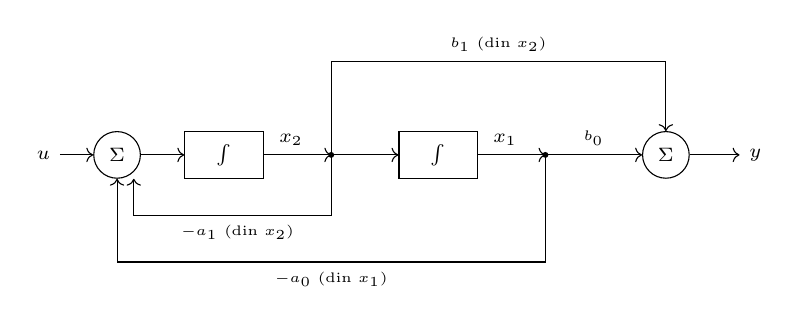
\begin{tikzpicture}[scale=0.85, every node/.style={font=\scriptsize}]
\node (u) at (0,0) {$u$};
\node[draw,circle,minimum size=0.5cm] (s1) at (1.1,0) {$\Sigma$};
\draw[->] (u)--(s1);
\node[draw,minimum width=1cm,minimum height=0.6cm] (i1) at (2.7,0) {$\int$};
\draw[->] (s1)--(i1);
\coordinate (a) at (4.3,0);
\draw[->] (i1) -- (a) node[above,pos=0.4]{$x_2$};
\filldraw (a) circle (1pt);
\node[draw,minimum width=1cm,minimum height=0.6cm] (i2) at (5.9,0) {$\int$};
\draw[->] (a) -- (i2);
\coordinate (b) at (7.5,0);
\draw[->] (i2) -- (b) node[above,pos=0.4]{$x_1$};
\filldraw (b) circle (1pt);
\node[draw,circle,minimum size=0.5cm] (sy) at (9.3,0) {$\Sigma$};
\draw[->] (b) -- (sy) node[midway,above]{\tiny $b_0$};
\draw[->] (a) -- ++(0,1.4) -| (sy.north);
\node[above] at (6.8,1.4){\tiny $b_1$ (din $x_2$)};
\draw[->] (sy) -- (10.4,0) node[right]{$y$};
\draw[->] (b) -- ++(0,-1.6) -| (s1.south);
\node[below] at (4.3,-1.6){\tiny $-a_0$ (din $x_1$)};
\draw[->] (a) -- ++(0,-0.9) -| ($(s1.south)+(0.25,0)$);
\node[below] at (2.9,-0.9){\tiny $-a_1$ (din $x_2$)};
\end{tikzpicture}
\end{center}
Ordinul $n$ mai mare $\Rightarrow$ mai multe integratoare în cascadă, aceeași logică (fiecare stare intermediară se ramifică spre sumatorul de reacție și, dacă $C$ are termen nenul pe poziția ei, spre sumatorul de ieșire).

\tip{\textbf{Notă — realizare generală (nu canonică):} fiecare stare $x_i$ are propriul sumator de reacție, cu gainuri $A_{i1},\dots,A_{in}$ (nu doar ultima linie). Exemplu: RLC din \hyperref[sec:1]{secțiunea 1}, unde $\dot x_1={-}\tfrac RLx_1-\tfrac1Lx_2+\tfrac1Lu$ (3 termeni $\to$ sumator) dar $\dot x_2=\tfrac1Cx_1$ (un singur termen $\to$ integrare directă, fără sumator).}

\section*{4c. Reducerea schemelor bloc cu bucle multiple — formula lui Mason (grafuri de fluență)}\phantomsection\label{sec:4c}
\srcnote{tehnică generală de teoria sistemelor, nu apare explicit în setul de cursuri TS2 disponibil — necesară pentru scheme cu mai mult de o buclă (vezi aplicarea completă la Subiectul 3, \hyperref[sec:22]{secțiunea 22}).}
Când o schemă bloc are \textbf{mai multe bucle care se suprapun} (nu se pot reduce una câte una, din exterior spre interior, fără ambiguitate), cea mai sigură metodă e formula lui Mason, aplicată pe graful de fluență al schemei (fiecare bloc = o ramură cu „câștig", fiecare sumator/nod = un nod al grafului):
\begin{keyeq}\color{red!65!black}
$$T=\dfrac YR=\dfrac1\Delta\sum_k P_k\Delta_k,\qquad \Delta=1-\sum_i L_i+\sum_{i,j}L_iL_j-\sum_{i,j,k}L_iL_jL_k+\cdots$$
\end{keyeq}
unde $P_k$ = câștigul căii directe (\textit{forward path}) $k$ (produsul blocurilor de la $R$ la $Y$, fără să repeți vreun nod); $L_i$ = câștigul buclei $i$ (produsul blocurilor parcurse pe buclă, cu semnul reacției inclus); sumele din $\Delta$ se fac pe TOATE combinațiile de bucle care \textbf{nu se ating} (nu au niciun nod comun) — perechi, apoi triplete etc; $\Delta_k$ = $\Delta$ recalculat păstrând DOAR buclele care NU ating calea $P_k$ (dacă $P_k$ atinge toate buclele, $\Delta_k{=}1$).

\textit{Rețetă practică:}
\begin{enumerate}
\item identifici toate căile directe $R\to Y$ (fără să treci de două ori prin același nod) — le înmulțești blocurile de pe fiecare, cu semn;
\item identifici toate buclele închise din schemă (fiecare buclă = revii la nodul de plecare) — înmulțești blocurile de pe ea, cu semnul reacției (de regulă $-$);
\item verifici, pentru fiecare PERECHE de bucle, dacă au vreun nod comun — dacă NU au, produsul lor intră cu $+$ în $\Delta$;
\item calculezi $\Delta$ (pasul 3) și, pentru fiecare cale $P_k$, $\Delta_k$ (la fel, dar ignorând buclele care ating acea cale);
\item aduni $P_k\Delta_k$ pentru toate căile și împarți la $\Delta$.
\end{enumerate}
\tip{\textit{Verificare utilă:} pentru o schemă cu o SINGURĂ buclă, formula se reduce exact la regula cunoscută $T{=}\dfrac{G}{1-L}$ (calea directă $P{=}G$, o singură buclă $L$, $\Delta{=}1{-}L$, $\Delta_1{=}1$) — deci formula lui Mason e o generalizare, nu o metodă nouă separată.}

\section*{5. Controlabilitate și observabilitate}\phantomsection\label{sec:5}
\srcnote{curs 3, secțiunile 6.5.1–6.5.2.}
\begin{keyeq}\color{red!65!black}
\textbf{Controlabilitate:} $P=[B\ \ AB\ \ A^2B\ \cdots\ A^{n-1}B]$, sistem controlabil $\iff \mathrm{rang}\,P=n\iff\det P\ne0$.

\textbf{Observabilitate:} $Q=\begin{pmatrix}C\\CA\\\vdots\\CA^{n-1}\end{pmatrix}$, sistem observabil $\iff \mathrm{rang}\,Q=n\iff\det Q\ne0$.
\end{keyeq}
\textbf{Reguli rapide:} un sistem cu variabile de fază (forma complet controlabilă) e \textbf{întotdeauna controlabil} (prin construcție) și, de regulă, și \textbf{observabil} (cursul afirmă acest lucru necondiționat; excepția cu simplificări pol-zero în $G(s)$ e o precizare suplimentară, corectă teoretic, dar în plus față de curs). Verificare alternativă (calitativă): controlabil $\iff$ în graful de fluență există cale de la $u$ la toate stările; observabil $\iff$ există cale de la toate stările la $y$.

\section*{6. Răspunsul în frecvență}\phantomsection\label{sec:6}
\srcnote{curs 4, secțiunea 4.1.1.}
Pentru $u(t)=U\sin\omega t$ aplicat unui sistem liniar stabil $G(s)$, răspunsul \textbf{staționar} este:
\begin{keyeq}\color{red!65!black}
$$y_{st}(t)=U|G(j\omega)|\sin[\omega t+\varphi(\omega)]=Y\sin(\omega t+\varphi),\qquad G(j\omega)=G(s)|_{s=j\omega}=A(\omega)e^{j\varphi(\omega)}$$
$$A(\omega)=|G(j\omega)|,\qquad \varphi(\omega)=\arg G(j\omega)=\mathrm{arctg}\dfrac{\mathrm{Im}\{G(j\omega)\}}{\mathrm{Re}\{G(j\omega)\}}$$
\end{keyeq}
$\varphi<0$ = întârziere de fază; $\varphi>0$ = avans de fază. \textbf{Avantaj Nyquist/frecvență:} evaluează stabilitatea în circuit închis doar din $G(j\omega)H(j\omega)$ în circuit deschis, fără a calcula rădăcinile ecuației caracteristice.

\section*{7. Caracteristici Bode — factorii de bază}\phantomsection\label{sec:7}
\srcnote{curs 4, secțiunea 4.2 (intro) + curs 5, secțiunea 4.2.1 (toate regulile de mai jos).}
$A_{dB}(\omega)=20\lg|G(j\omega)|$; \textbf{octavă} $=[\omega_1,2\omega_1]$, \textbf{decadă} $=[\omega_1,10\omega_1]$.
\begin{keyeq}\color{red!65!black}
\textbf{Factor de amplificare $K$:} dreaptă orizontală la $K_{dB}=20\lg K$; fază $=0$.

\textbf{Integrator $(j\omega)^{-1}$:} pantă $-20$dB/decadă (trece prin $0$dB la $\omega{=}1$); fază $=-90^\circ$ constant. \textbf{Derivator $j\omega$:} pantă $+20$dB/decadă; fază $=+90^\circ$.

\textbf{Ordinul unu $1/(1+j\omega T)$:} asimptotă $0$dB pentru $\omega<1/T$; pantă $-20$dB/dec pentru $\omega>1/T$; frecvența de frângere $\omega_f=1/T$ (eroare max. $-3$dB la $\omega_f$); fază $-\mathrm{arctg}(\omega T)$: $0^\circ\to-45^\circ$ (la $\omega_f$) $\to-90^\circ$; aproximare 3 drepte: $0^\circ$ până la $\omega_f/10$, pantă $-45^\circ$/dec până la $10\omega_f$, apoi $-90^\circ$. \textbf{Factorul invers $(1+j\omega T)$:} oglindă (semn schimbat) — pantă $+20$dB/dec, fază $0^\circ\to+90^\circ$. \textbf{Denumiri} (curs 5): fiindcă $1/(1{+}j\omega T)$ are fază negativă, se numește element de ordinul unu \textbf{cu întârziere de fază}; factorul invers $(1{+}j\omega T)$, cu fază pozitivă, se numește, alternativ, element \textbf{cu anticipare de fază} (avans de fază) — exact cazul din Subiectul 2, \hyperref[sec:20]{secțiunea 20} ($G(s){=}20(s{+}1)/(s{+}2)$, zero înainte de pol).

\textbf{Ordinul $n$, $(1+j\omega T)^{\pm n}$:} pantă $\mp20n$dB/dec, aceeași $\omega_f$, eroare de $n$ ori mai mare.

\textbf{Ordinul doi $[1+2\zeta(j\omega/\omega_n)+(j\omega/\omega_n)^2]^{-1}$:} asimptotă $0$dB pentru $\omega<\omega_n$, pantă $-40$dB/dec pentru $\omega>\omega_n$ (frecvența de frângere $=\omega_n$, independent de $\zeta$); vârf de rezonanță lângă $\omega_n$ dacă $\zeta$ mic; fază $0^\circ\to-90^\circ$ (la $\omega_n$) $\to-180^\circ$. Aproximare fază: dacă $\zeta>0{,}4$ — 3 drepte ($0^\circ$ până la $\omega_n/10$, pantă $-90^\circ$/dec, $-180^\circ$ după $10\omega_n$); dacă $\zeta<0{,}4$ — treaptă verticală la $\omega_n$ de la $0^\circ$ la $-180^\circ$. \textbf{Factor invers (la numărător):} semn schimbat (simetric față de axa pulsațiilor).
\end{keyeq}

\section*{8. Algoritmul de trasare a diagramelor Bode}\phantomsection\label{sec:8}
\srcnote{curs 6, secțiunea 4.2.2.}
Se scrie $G(s)H(s)$ în \textbf{forma standard (monică)} cu factori $(sT+1)$, $(j\omega)^{\pm1}$, pătratici.
\begin{enumerate}
\item se dispun pe axa $\omega$ (log) toate frecvențele de frângere, crescător;
\item \textbf{modul:} se trasează asimptota fiecărui factor (regulile \hyperref[sec:7]{secțiunii 7}); se plasează punctul $(1,K_{dB})$, asimptotă joasă frecvență cu panta $-20\,$(tip)$\,$dB/dec (tip = nr. integratoare); la fiecare frecvență de frângere panta se modifică cu $\pm20$ sau $\pm40$dB/dec; se corectează cu $\pm3$dB (ordin 1) sau $\pm20\lg(1/2\zeta)$ (ordin 2, vârf la numitor / vale la numărător);
\item \textbf{fază:} pentru fiecare factor se marchează $\omega_f/10$ și $10\omega_f$; asimptotă joasă frecvență la $-90^\circ\cdot$(tip); se însumează grafic fazele individuale ale tuturor factorilor.
\end{enumerate}

\section*{9. Caracteristici polare (locul de transfer / Nyquist)}\phantomsection\label{sec:9}
\srcnote{curs 6, secțiunea 4.3.}
Reprezentarea în plan complex a $G(j\omega)$ când $\omega:0\to\infty$; unghi pozitiv = sens trigonometric.
\begin{keyeq}\color{red!65!black}
\textbf{Comportare la $\omega\to0$, după tipul $\nu$ (nr. integratoare din $G(s)H(s)$):}
\begin{itemize}
\item tip $0$: punct de start \textbf{finit}, pe semiaxa reală pozitivă, tangentă $\perp$ axa reală;
\item tip $1$: modul $\to\infty$, fază $\to-90^\circ$ — asimptotă paralelă cu semiaxa imaginară negativă;
\item tip $2$: modul $\to\infty$, fază $\to-180^\circ$ — asimptotă paralelă cu semiaxa reală negativă.
\end{itemize}
\textbf{Comportare la $\omega\to\infty$ (dacă $n-m$ = grad numitor $-$ grad numărător):} converge spre origine, tangent la o semiaxă, în sens orar — $n{-}m{=}1\Rightarrow$ tangent semiaxa imaginară negativă; $n{-}m{=}2\Rightarrow$ semiaxa reală negativă; $n{-}m{=}3\Rightarrow$ semiaxa imaginară pozitivă.
\end{keyeq}
\textbf{Tabel forme uzuale:} $1/(j\omega)\to$ semiaxa imaginară negativă (dreaptă); $1/(j\omega)^2\to$ semiaxa reală negativă; $K(1+j\omega T_1)/(j\omega T_2)\to$ dreaptă verticală (tip 1, numărător ordin 1); $K/[(1+j\omega T_1)(1+j\omega T_2)]\to$ semicerc în cadranul IV; $K/[j\omega(1+j\omega T_1)(1+j\omega T_2)]\to$ pornește vertical (tip1), se curbează prin cadranul III spre origine. Forma la $\omega$ medii/mari depinde puternic de constantele de timp de la \textbf{numărător}.

\section*{10. Criteriul de stabilitate Nyquist}\phantomsection\label{sec:10}
\srcnote{curs 7, secțiunea 4.5 (4.5.2 formă simplificată, 4.5.3 formă generală).}
\textbf{Principiul argumentului:} un contur $C_s$ din planul $s$ care încercuiește orar $Z$ zerouri și $P$ poli ai $F(s)$ (fără să treacă prin ei) $\Rightarrow$ conturul imagine $C_F$ încercuiește originea de $N=Z-P$ ori, orar.

\textbf{Conturul Nyquist:} axa $j\omega$ ($-\infty\to\infty$) $+$ semicerc de rază infinită în semiplanul drept — încercuiește tot semiplanul drept. Aplicat lui $F(s)=1+G(s)H(s)$: $Z$ zerouri ale lui $F(s)$ = poli instabili ai sistemului închis.
\begin{keyeq}\color{red!65!black}
\textbf{Echivalență cheie:} încercuirea originii de curba $1+G(j\omega)H(j\omega)$ $\equiv$ încercuirea punctului \textbf{critic $-1+j0$} de curba polară a $G(j\omega)H(j\omega)$.

\textbf{Formă simplificată} ($P=0$, sistem deschis stabil): sistem închis stabil $\iff$ locul $G(j\omega)H(j\omega)$ ($\omega:0\to\infty$) \textbf{nu încercuiește} $-1+j0$ (rămâne la dreapta lui, dacă parcurgi curba în sensul crescător al lui $\omega$).

\textbf{Formă generală} ($P\ne0$ poli instabili în circuit deschis): sistem închis stabil $\iff$ locul de transfer încercuiește $-1+j0$ exact de $P$ ori, în sens trigonometric (antiorar).
\end{keyeq}

\section*{11. Stabilitatea relativă — margini de amplitudine și fază}\phantomsection\label{sec:11}
\srcnote{curs 8, secțiunea 4.6 (rel. 4.38–4.39).}
(reacție negativă unitară, $G(s)$ fără poli/zerouri în semiplanul drept)
\begin{keyeq}\color{red!65!black}
$$\omega_t:\ |G(j\omega_t)|=1\ \text{(pulsația de tăiere)}\qquad\quad \omega_\pi:\ \angle G(j\omega_\pi)=-180^\circ\ \text{(pulsația de fază)}$$
$$m_a=\dfrac{1}{|G(j\omega_\pi)|}\ \ (m_{a,dB}=-20\lg|G(j\omega_\pi)|)\qquad\qquad \gamma=180^\circ+\angle G(j\omega_t)$$
\end{keyeq}
\textbf{Sistem stabil} $\iff m_a>1$ ($m_{a,dB}>0$) \textbf{și} $\gamma>0$ (echivalent $\omega_t<\omega_\pi$). Pe Bode: $\omega_t$ = intersecția modulului cu $0$dB; $\omega_\pi$ = intersecția fazei cu $-180^\circ$. Sistemele de ordinul 1 și 2 au $m_a=\infty$ (curba polară nu taie semiaxa reală negativă) $\Rightarrow$ teoretic nu pot fi instabile (buclă unitară).

\section*{12. Indicatori de calitate în domeniul frecvenței}\phantomsection\label{sec:12}
\srcnote{curs 8, secțiunea 4.7 (rel. 4.33, 4.34, 4.41, 4.42).}
Pentru $G_0(j\omega)=\dfrac{G(j\omega)}{1+G(j\omega)}$ (circuit închis, reacție unitară), $M(\omega)=|G_0(j\omega)|$:
\begin{keyeq}\color{red!65!black}
\textbf{Vârf de rezonanță} (doar sistem ordin 2, $\zeta\le0{,}707$): $\omega_r=\omega_n\sqrt{1-2\zeta^2}$, $\;M_r=\dfrac{1}{2\zeta\sqrt{1-\zeta^2}}$ (dacă $\zeta>0{,}707$: nu există rezonanță, $M_r=1$).

\textbf{Lărgime de bandă} $\omega_b$: $M(\omega_b)=0{,}707\,M(0)$ (adică $-3$dB față de $M(0)$). Pentru ordin 2: $\omega_b=\omega_n\sqrt{1-2\zeta^2+\sqrt{2-4\zeta^2+4\zeta^4}}$; aproximare uzuală ($\zeta\in[0{,}5;0{,}8]$): $\omega_b\approx\omega_n(1{,}5-\zeta^2)$ (sau, simplu, $\omega_b\approx\omega_n$ dacă $\zeta=\sqrt2/2$).
\end{keyeq}
$M_r$ mare $\Rightarrow$ poli dominanți slab amortizați $\Rightarrow$ răspuns oscilant; $M_r\approx1\Rightarrow$ bine amortizat. Bandă mare $\Rightarrow$ urmărire bună a intrării, dar sensibilitate mai mare la zgomot + cost hardware.

\section*{12b. Indicatori de calitate în domeniul timpului (răspuns la treaptă, ordinul doi)}\phantomsection\label{sec:12b}
\srcnote{recapitulare TS1 (formule standard pentru răspunsul tranzitoriu al sistemelor de ordinul doi — capitol din setul TS1, scanat, fără text extractabil; formulele sunt cele consacrate, folosite deja la Subiectul 2d, \hyperref[sec:22]{secțiunea 22}).}
Pentru un sistem de ordinul doi standard, subamortizat ($0{<}\zeta{<}1$), $G_0(s)=\dfrac{\omega_n^2}{s^2+2\zeta\omega_ns+\omega_n^2}$, răspunsul la treaptă unitară oscilează amortizat în jurul valorii finale $1$, caracterizat de patru indicatori:
\begin{keyeq}\color{red!65!black}
$$\sigma=e^{-\pi\zeta/\sqrt{1-\zeta^2}}\cdot100\%\ \text{(suprareglaj)},\qquad t_p=\dfrac\pi{\omega_d}\ \text{(timp de vârf)},\qquad \omega_d=\omega_n\sqrt{1-\zeta^2}$$
$$t_s\approx\dfrac4{\zeta\omega_n}\ \text{(timp de stabilizare, criteriul 2\%)},\qquad t_r\approx\dfrac{1{,}8}{\omega_n}\ \text{(timp de creștere, aproximare uzuală)}$$
\end{keyeq}
\textbf{Legătura cu $\zeta,\omega_n$:} cu cât $\zeta$ e mai mic, cu atât $\sigma$ e mai mare (mai oscilant) — la $\zeta{\to}0$, $\sigma{\to}100\%$; la $\zeta{\ge}1$ (critic/supraamortizat) nu mai există depășire, deci $\sigma,t_p$ nu se definesc (răspunsul e monoton, \hyperref[sec:22]{secțiunea 22}, Teorie pct. 3). $t_s$ și $t_r$ scad amândouă dacă $\omega_n$ crește (sistem „mai rapid"), independent de $\zeta$.

\textit{Formula exactă a răspunsului} (dacă ai nevoie de expresia completă $y(t)$, nu doar de indicatori):
$$y(t)=1-\dfrac1{\sqrt{1-\zeta^2}}\,e^{-\zeta\omega_nt}\sin(\omega_dt+\theta),\qquad \theta=\arccos\zeta$$

\section*{13. Sisteme multivariabile — introducere}\phantomsection\label{sec:13}
\srcnote{curs 9, capitolul „Sisteme multivariabile" (rel. 6.1–6.3).}
Pentru 2 intrări/2 ieșiri (buclele considerate decuplate — celelalte intrări $=0$ la proiectarea unei legi de reglare):
\begin{keyeq}\color{red!65!black}
$$Y_1(s)=G_{11}(s)U_1(s)+G_{12}(s)U_2(s),\quad Y_2(s)=G_{21}(s)U_1(s)+G_{22}(s)U_2(s)$$
$$G_p(s)=\begin{pmatrix}G_{11}&G_{12}\\G_{21}&G_{22}\end{pmatrix}\qquad \textbf{factorul de cuplare: } K_0=\dfrac{G_{12}(0)G_{21}(0)}{G_{11}(0)G_{22}(0)}=\dfrac{K_{12}K_{21}}{K_{11}K_{22}}$$
\end{keyeq}
$G_{11},G_{22}$ = funcții de transfer principale; $G_{12},G_{21}$ = funcții de cuplare (interacțiune între bucle). $K_0\to0$ = cuplaj slab (bucle aproape independente).

\section*{14. Locul rădăcinilor — condiții și cei 8 pași}\phantomsection\label{sec:14}
\srcnote{curs 10, secțiunile 5.1, 5.1.1, 5.2 (rel. 5.1–5.10, regulile 1–8).}
Ecuația caracteristică $1+G(s)H(s)=0\Leftrightarrow G(s)H(s)=-1=1\cdot e^{j(2k+1)180^\circ}$:
\begin{keyeq}\color{red!65!black}
\textbf{condiția modulului:} $|G(s)H(s)|=1$ \qquad \textbf{condiția argumentului:} $\angle G(s)H(s)=180^\circ(2k+1)$
\end{keyeq}
Locul = poziția polilor sistemului închis când $K:0\to\infty$ în $1+K\dfrac{(s-z_1)\cdots(s-z_m)}{(s-p_1)\cdots(s-p_n)}=0$.

\begin{enumerate}
\item ecuația caracteristică, se izolează $K$ ca factor; se plasează polii/zerourile lui $G(s)H(s)$ (simetrie față de axa reală);
\item \textbf{nr. ramuri} $=n$; locul \textbf{pleacă din poli} ($K{=}0$) și \textbf{se termină în zerouri} (finite sau la $\infty$, $K{\to}\infty$); $m$ ramuri merg spre zerourile finite, $n{-}m$ spre asimptote;
\item pe axa reală: aparține locului porțiunea la \textbf{dreapta} căreia se află un \textbf{număr impar} de poli+zerouri reale (perechile complexe nu contează, fază $360^\circ$);
\item \textbf{asimptote:} nr. $=n-m$; $\theta_k=\dfrac{180^\circ(2k+1)}{n-m}$; centrul $\sigma_a=\dfrac{\sum p_i-\sum z_j}{n-m}$ (mereu real);
\item \textbf{unghi de plecare} dintr-un pol complex: $\varphi_p=180^\circ-\sum(\text{unghiuri de la ceilalți poli})+\sum(\text{unghiuri de la zerouri})$; \textbf{unghi de sosire} într-un zero complex: $\varphi_s=180^\circ-\sum(\text{unghiuri de la celelalte zerouri})+\sum(\text{unghiuri de la poli})$;
\item \textbf{puncte de ramificație:} rădăcinile reale (de pe porțiunea din pasul 3) ale $\dfrac{dK}{ds}=0$, cu $K=-A(s)/B(s)$;
\item \textbf{intersecția cu axa imaginară:} criteriul Routh (rând $=0$ complet — cum se construiește tabloul: \hyperref[sec:14b]{secțiunea 14b}) sau înlocuind $s=j\omega$ în ecuația caracteristică, rezolvând Re/Im $=0$ pentru $\omega,K$;
\item \textbf{gradare:} $K=\dfrac{\text{produsul distanțelor de la }s\text{ la poli}}{\text{produsul distanțelor de la }s\text{ la zerouri}}$.
\end{enumerate}
\tip{\textit{Observație:} dacă $n-m\ge2$, suma rădăcinilor ($=-a_{n-1}$) e independentă de $K$ — dacă o ramură se deplasează spre stânga când $K$ crește, alta compensează spre dreapta.}

\begin{center}
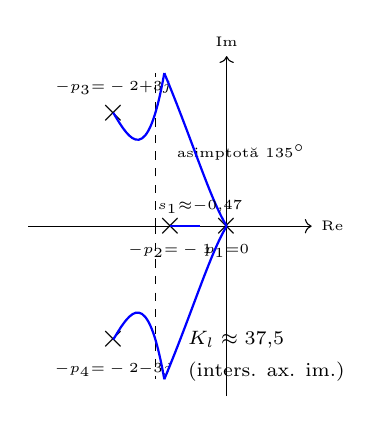
\begin{tikzpicture}[scale=0.72]
\draw[->] (-3.5,0) -- (1.5,0) node[right]{\tiny Re};
\draw[->] (0,-3) -- (0,3) node[above]{\tiny Im};
\node at (0,0){\large$\times$}; \node[below] at (0,-0.15){\tiny $p_1{=}0$};
\node at (-1,0){\large$\times$}; \node[below] at (-1,-0.15){\tiny $-p_2{=}-1$};
\node at (-2,2){\large$\times$}; \node[above] at (-2,2.15){\tiny $-p_3{=}-2{+}3j$};
\node at (-2,-2){\large$\times$}; \node[below] at (-2,-2.25){\tiny $-p_4{=}-2{-}3j$};
\draw[dashed] (-1.25,0)--(-1.25,2.7); \draw[dashed] (-1.25,0)--(-1.25,-2.7);
\node[right] at (-1.05,1.3){\tiny asimptotă $135^\circ$};
\draw[thick,blue] (0,0) .. controls (-0.3,0.5) and (-0.6,1.5) .. (-1.1,2.7);
\draw[thick,blue] (0,0) .. controls (-0.3,-0.5) and (-0.6,-1.5) .. (-1.1,-2.7);
\draw[thick,blue] (-1,0) -- (-0.47,0);
\node[above] at (-0.47,0.05){\tiny $s_1{\approx}{-}0{,}47$};
\draw[thick,blue] (-2,2) .. controls (-1.7,1.5) and (-1.4,1) .. (-1.1,2.7);
\draw[thick,blue] (-2,-2) .. controls (-1.7,-1.5) and (-1.4,-1) .. (-1.1,-2.7);
\node[align=left] at (0.7,-2.3){\scriptsize $K_l\approx37{,}5$\\\scriptsize (inters. ax. im.)};
\end{tikzpicture}
\end{center}

\section*{14b. Criteriul Routh-Hurwitz — cum se construiește tabloul}\phantomsection\label{sec:14b}
\srcnote{criteriu general de stabilitate, folosit la pasul 7 din \hyperref[sec:14]{secțiunea 14} (intersecția locului cu axa $j\omega$) — aplicare completă la \hyperref[sec:15]{secțiunea 15}.}

Pornești de la ecuația caracteristică adusă la forma polinom (membrul drept $0$), ordonată descrescător după puterile lui $s$:
$$a_ns^n+a_{n-1}s^{n-1}+\cdots+a_1s+a_0=0$$

\textbf{Primele două rânduri} se scriu direct din coeficienți, alternând — rândul $s^n$ ia coeficienții de pe pozițiile pare (față de $a_n$), rândul $s^{n-1}$ pe cele impare:
\begin{center}
\begin{tabular}{c|cccc}
$s^n$ & $a_n$ & $a_{n-2}$ & $a_{n-4}$ & $\cdots$\\
$s^{n-1}$ & $a_{n-1}$ & $a_{n-3}$ & $a_{n-5}$ & $\cdots$
\end{tabular}
\end{center}

\textbf{Fiecare rând următor} se calculează din cele \textbf{două rânduri de deasupra}, element cu element — folosesc notația $[s^k]_j${=}elementul $j$ din rândul etichetat $s^k$ (aceleași etichete ca în tabel, ca să nu introduc litere noi). Pentru rândul $s^k$ (cu $k\le n{-}2$), folosind rândul imediat deasupra $s^{k+1}$ (\textbf{pivotul} e $[s^{k+1}]_1$, primul lui element) și rândul de deasupra acestuia, $s^{k+2}$:
\begin{keyeq}\color{red!65!black}
$$[s^k]_j=\dfrac{[s^{k+1}]_1\cdot[s^{k+2}]_{j+1}-[s^{k+2}]_1\cdot[s^{k+1}]_{j+1}}{[s^{k+1}]_1}=-\dfrac1{[s^{k+1}]_1}\begin{vmatrix}[s^{k+2}]_1 & [s^{k+2}]_{j+1}\\ [s^{k+1}]_1 & [s^{k+1}]_{j+1}\end{vmatrix},\qquad j=1,2,\dots$$
\end{keyeq}
— practic, "determinant $2\times2$ cu prima coloană a celor două rânduri de deasupra și coloana $j{+}1$, împărțit la pivot, cu semn schimbat". Așa au ieșit $b_1,c_1$ din \hyperref[sec:15]{secțiunea 15}: $b_1{=}[s^2]_1$ vine din $[s^4]_1{=}1$, $[s^4]_2{=}22$, $[s^3]_1{=}8$ (pivot), $[s^3]_2{=}24{+}K$; $c_1{=}[s^1]_1$ vine analog din rândurile $s^3,s^2$.

Continui până la rândul $s^0$ (un singur element, mereu $=a_0$, bun ca verificare finală). Tabloul are $n{+}1$ rânduri; elementele care lipsesc (rând mai scurt decât cele de sus) se consideră $0$.

\textbf{Exemplu generic, ordin 3} ($a_3s^3+a_2s^2+a_1s+a_0=0$):
\begin{center}
\begin{tabular}{c|cc}
$s^3$ & $a_3$ & $a_1$\\
$s^2$ & $a_2$ & $a_0$\\
$s^1$ & $\dfrac{a_2a_1-a_3a_0}{a_2}$ & \\
$s^0$ & $a_0$ &
\end{tabular}
\end{center}
(regăsit direct în \hyperref[sec:22]{secțiunea 22}: limita de stabilitate la ordin 3 e $a_2a_1{=}a_0$, adică exact numărătorul de mai sus $=0$.)

\textbf{Interpretare (criteriul de stabilitate):}
\begin{itemize}
\item sistemul e stabil $\iff$ \textbf{toate} elementele din prima coloană au același semn (de regulă toate pozitive, dacă $a_n{>}0$) — nicio schimbare de semn;
\item nr. de \textbf{schimbări de semn} în prima coloană $=$ nr. de rădăcini instabile (semiplanul drept);
\item dacă un rând iese \textbf{tot zero} (limita de stabilitate, cazul din \hyperref[sec:15]{secțiunea 15}): rândul de deasupra e "\textbf{polinomul auxiliar}" — rădăcinile lui (rezolvat direct ca ecuație în $s$) sunt exact punctele unde locul taie axa $j\omega$;
\item dacă doar \textbf{primul element} al unui rând e zero (dar nu tot rândul): îl înlocuiești temporar cu $\varepsilon{\to}0^+$, continui calculul normal, apoi analizezi semnele când $\varepsilon\to0$.
\end{itemize}

\tip{\textit{Rețetă rapidă pt. $K_l$ (limita de stabilitate în funcție de $K$), la polinoame de grad $\le4$:} pui condiția ca rândul $s^1$ să se anuleze — de regulă o ecuație liniară sau pătratică în $K$ — rezolvi și obții $K_l$. Apoi înlocuiești $K_l$ înapoi în rândul $s^2$ (polinomul auxiliar $b_1s^2{+}b_2{=}0$) ca să afli $\omega$ la intersecția cu axa $j\omega$: $s^2{=}-b_2/b_1\Rightarrow s{=}\pm j\omega$.}

\section*{15. Locul rădăcinilor — exemplu numeric complet}\phantomsection\label{sec:15}
\srcnote{curs 11, primul exemplu rezolvat (Fig. 5.T4) — aceleași date numerice, aplicare directă.}
\textit{Aplicarea directă, pas cu pas, a rețetei din \hyperref[sec:14]{secțiunea 14}}, pentru $G(s)=\dfrac{K}{s(s+1)(s^2+4s+13)}$ (reacție unitară). \textbf{1)} (pasul 1) poli: $p_1{=}0,\,{-}p_2{=}{-}1,\,{-}p_{3,4}{=}{-}2{\pm}3j$; fără zerouri finite. \textbf{2)} (pasul 2, nr. ramuri$=n$) $n{=}4\Rightarrow$ 4 ramuri. \textbf{3)} (pasul 3, regula parității impare) axa reală: $(-1,0)$. \textbf{4)} (pasul 4, $\theta_k{=}\tfrac{180^\circ(2k+1)}{n-m}$) $n{-}m{=}4\Rightarrow$ asimptote la $\theta=\pm45^\circ,\pm135^\circ$. \textbf{5)} (pasul 4, $\sigma_a{=}\tfrac{\sum p_i-\sum z_j}{n-m}$) centru asimptote $\sigma_a=\dfrac{0-1-2-2}{4}=-1{,}25$. \textbf{6)} (pasul 5, $\varphi_p{=}180^\circ{-}\sum\text{unghiuri poli}{+}\sum\text{unghiuri zerouri}$) unghi plecare din $-p_3{=}-2{+}3j$: unghiurile vectorilor de la ceilalți poli $\approx123{,}7^\circ,108{,}5^\circ,90^\circ\Rightarrow \varphi_p=180-(123{,}7+108{,}5+90)=-142{,}2^\circ$ (simetric $+142{,}2^\circ$ pt. $-p_4$). \textbf{7)} (pasul 6, $dK/ds{=}0$ cu $K{=}{-}A(s)/B(s)$) punct ramificație: $K=-s(s+1)(s^2+4s+13)$, $dK/ds=0\Rightarrow4s^3+15s^2+34s+13=0\Rightarrow s_1\approx-0{,}47$ (singura rădăcină reală). \textbf{8)} (pasul 7, Routh sau $s{=}j\omega$) $K_l$ la limita de stabilitate: ecuație caracteristică $s^4+5s^3+17s^2+13s+K=0$, tablou Routh $\Rightarrow 13-\dfrac{25K}{72}=0\Rightarrow K_l\approx37{,}5$.

\section*{16. Sisteme neliniare — tipuri de neliniarități}\phantomsection\label{sec:16}
\srcnote{curs 12, secțiunea 5.1 (Tabelul 5.1, rel. 5.3–5.6).}
Sistem neliniar $\iff$ conține $\ge1$ element neliniar; \textbf{nu se aplică suprapunerea efectelor}: $y(a_1u_1+a_2u_2)\ne a_1y_1+a_2y_2$ în general. \textbf{Neliniarități esențiale} = neanalitice, cu punct singular — \textbf{nu pot fi liniarizate} (ex: releu ideal).
\begin{keyeq}\color{red!65!black}
\textbf{Tipuri statice uzuale} (caracteristică $y=f(u)$): \textbf{saturație} ($y{=}Ku$ pt.$|u|{<}\beta$, $y{=}M\,\mathrm{sign}(u)$ altfel); \textbf{zonă de insensibilitate} (mort la $|u|{<}\beta$); \textbf{zonă insensibilitate + saturație}; \textbf{amplificări diferite pe zone}; \textbf{releu ideal} ($y=M\,\mathrm{sign}(u)$); \textbf{releu cu insensibilitate}; \textbf{releu cu histerezis} (neliniaritate \textbf{cu memorie} — depinde de $y(t-\varepsilon)$, nu doar de $u(t)$); \textbf{joc în transmisia mecanică}.
\end{keyeq}
Model general: $\dot x=f(x,u,t)$, $y=g(x,t)$ (sau, dacă se neglijează perturbațiile: $\dot x=f(x,u)$, $y=g(x)$ — invariant în timp). \textbf{Polaritate directă:} $u(t)y(t)\ge0\ \forall t$ (caracteristica e în cadranele I și III) — condiție utilă la evaluarea stabilității.

\section*{17. Liniarizarea modelelor neliniare}\phantomsection\label{sec:17}
\srcnote{curs 13.}
Se aproximează $f(x)$ prin \textbf{serie Taylor} în jurul punctului static de funcționare $x_s$, neglijând termenii de ordin superior:
\begin{keyeq}\color{red!65!black}
$$f(x)\approx f(x_s)+\dfrac{\partial f}{\partial x}\bigg|_{x_s}(x-x_s)\qquad\text{(1 variabilă)}$$
$$\dot{\bar x}=A\bar x+B\bar u,\quad \bar y=C\bar x,\qquad A=\left[\dfrac{\partial f_i}{\partial x_j}\right]_{x_s,u_s}\ (\text{Jacobian}),\ B=\left[\dfrac{\partial f_i}{\partial u_j}\right]_{x_s,u_s},\ \bar x=x-x_s,\ \bar u=u-u_s$$
\end{keyeq}
\textbf{Pași:} (1) se scriu ecuațiile de stare neliniare $\dot x=f(x,u)$; (2) se determină punctul de echilibru $x_s$ (regim staționar, $\dot x=0$); (3) se calculează Jacobianul $A=\partial f/\partial x$ evaluat în $x_s$ (și $B=\partial f/\partial u$); (4) modelul liniarizat e valabil doar \textbf{local}, în jurul lui $x_s$.

\textbf{Exemplu 1 (pendul):} $\ell\ddot\theta+g\sin\theta=0$; pentru $\theta$ mic, $\sin\theta\approx\theta\Rightarrow\ell\ddot\theta+g\theta=0$ (liniarizare directă, echilibru $\theta_s=0$).

\textbf{Exemplu 2} — sistem cu $\dot x_1=x_2+u=f_1$, $\dot x_2=-x_1+x_1^2=f_2$, $y=x_2$:
$$A=\begin{pmatrix}\partial f_1/\partial x_1&\partial f_1/\partial x_2\\\partial f_2/\partial x_1&\partial f_2/\partial x_2\end{pmatrix}=\begin{pmatrix}0&1\\-1+2x_1&0\end{pmatrix}$$
la echilibrul $(x_{1s},x_{2s})=(0,0)$: $A=\begin{pmatrix}0&1\\-1&0\end{pmatrix}$, $B=\begin{pmatrix}1\\0\end{pmatrix}$ — sistem liniarizat $\dot{\bar x}_1=\bar x_2+\bar u,\ \dot{\bar x}_2=-\bar x_1$. La echilibrul $(1,0)$: $A=\begin{pmatrix}0&1\\1&0\end{pmatrix}$ (alt comportament — poli $\pm1$, instabil local!).

\textbf{Exemplu 3 (nivelul lichidului într-un rezervor de secțiune $A$, ieșire liberă $Q_e=\alpha\sqrt{2gL}$):} regim static $Q_a{=}Q_e$; dinamic $Q_a(t)-Q_e(t)=A\dfrac{dL(t)}{dt}$. Liniarizând $Q_e(L)$ în jurul lui $L_0$: $Q_e(t)\approx Q_e(L_0)+\dfrac{\partial Q_e}{\partial L}\Big|_{L_0}(L(t)-L_0)=bL(t)+\text{ct.}\Rightarrow Q_a(s)-bL(s)=AsL(s)\Rightarrow G(s)=\dfrac{L(s)}{Q_a(s)}=\dfrac{1}{As+b}$ (fără liniarizare, cu $Q_e=\alpha\sqrt{2gL}$ direct: $G(s)=1/(As)$, integrator pur).

\section*{18. Eroarea staționară (sisteme continue)}\phantomsection\label{sec:18}
\srcnote{Seminarii, secțiunea 4.2.3 („Corelații între erorile staționare și caracteristica modulului") — nu apare în niciun curs din setul disponibil (cursul de bază, cap. 3, nu e inclus); coeficienții $K_p,K_v,K_a$ sunt standard, consistenți cu ce se derivă acolo.}
Pentru reacție negativă cu $G(s)H(s)$ în circuit deschis, eroarea $E(s)=\dfrac{R(s)}{1+G(s)H(s)}$. Cu \textbf{teorema valorii finale} (necesită $sE(s)$ stabilă, fără poli în SCD sau pe axa $j\omega$):
\begin{keyeq}\color{red!65!black}
$$e_{ss}=\lim_{t\to\infty}e(t)=\lim_{s\to0}sE(s)=\lim_{s\to0}\dfrac{sR(s)}{1+G(s)H(s)}$$
\end{keyeq}
\textbf{Tipul sistemului} $\nu$ = nr. de poli ai $G(s)H(s)$ în $s{=}0$ (nr. integratoare). \textbf{Coeficienți de eroare:}
\begin{itemize}
\item treaptă $R(s){=}1/s$: $e_{ss}=\dfrac{1}{1+K_p}$, $K_p=\lim_{s\to0}G(s)H(s)$ — finit (deci $e_{ss}{>}0$) doar la tip $0$; la tip $\ge1$: $e_{ss}=0$;
\item rampă $R(s){=}1/s^2$: $e_{ss}=1/K_v$, $K_v=\lim_{s\to0}sG(s)H(s)$ — finit la tip $1$; $e_{ss}{=}0$ la tip $\ge2$; $e_{ss}{=}\infty$ la tip $0$;
\item parabolă $R(s){=}1/s^3$: $e_{ss}=1/K_a$, $K_a=\lim_{s\to0}s^2G(s)H(s)$ — finit la tip $2$.
\end{itemize}
\tip{\textit{Practic:} se scrie direct $sR(s)/[1+G(s)H(s)]$ și se calculează limita — nu trebuie memorate $K_p,K_v,K_a$.}

\tip{\textbf{Metodă alternativă — citire directă de pe graficul Bode} (Seminarii, secțiunea 4.2.3): dacă ai deja desenat modulul logaritmic (ex. de la Subiectul 2 din orice bilet), nu mai trebuie să calculezi limita separat — constantele de eroare se citesc direct din asimptota de joasă frecvență:
\begin{itemize}
\item \textbf{tip 0:} asimptota de joasă frecvență e orizontală, la nivelul $K_{dB}{=}20\lg K$; $K_p{=}K$ (citești direct înălțimea platoului).
\item \textbf{tip 1:} asimptota de joasă frecvență are panta $-20$dB/dec; prelungind-o (sau citind direct, dacă trece prin grafic) până unde taie linia de $0$dB, frecvența de tăiere $\omega_0$ a ACELEI asimptote (nu neapărat a curbei exacte, dacă zero-ul e mai departe) e chiar $K_v$: din $20\lg(K/\omega_0){=}0\Rightarrow K/\omega_0{=}1\Rightarrow K_v{=}K{=}\omega_0$.
\item \textbf{tip 2:} asimptota de joasă frecvență are panta $-40$dB/dec; unde taie $0$dB (frecvența $\omega_a$) dă $K_a{=}\omega_a^2$ (din $20\lg[K/\omega_a^2]{=}0\Rightarrow\omega_a{=}\sqrt K{=}\sqrt{K_a}$).
\end{itemize}}
\tip{\textit{Exemplu deja desenat:} la Subiectul 2 din \hyperref[sec:19]{secțiunea 19} ($G(s){=}5(0{,}1s{+}1)/s$, tip $1$), graficul modulului are marcat exact punctul $(\omega{=}5,\,0\text{dB})$ — acela ESTE $K_v{=}5$, citit direct, fără să mai calculezi $\lim_{s\to0}sG(s)$.}

\textbf{Exemplu} ($G(s)=5\dfrac{0{,}1s+1}{s}$, reacție unitară, tip $1$): $K_p=\lim_{s\to0}G(s)=\infty\Rightarrow e_{ss}(\text{treaptă})=0$. $K_v=\lim_{s\to0}sG(s)=\lim_{s\to0}5(0{,}1s+1)=5\Rightarrow e_{ss}(\text{rampă})=1/K_v=0{,}2$.

\section*{19. Bilet oficial recent (sesiunea vară 2026) — formatul actual al examenului, foarte important!}\phantomsection\label{sec:19}
\textit{Bilet dat efectiv în acest an universitar; structura (5 subiecte + 4 întrebări de teorie, 1p fiecare) e cea mai probabilă pentru examenul curent, chiar dacă biletele mai vechi din \hyperref[sec:21]{secțiunea 21} rămân utile ca exerciții suplimentare.}

\textbf{Subiect 1 — $G_0(s)=\dfrac{s+5}{s^2+6s+9}=\dfrac{s+5}{(s+3)^2}$:}

\textbf{a) Model la stare} (realizare complet controlabilă, \hyperref[sec:4]{secțiunea 4a}):

Pentru orice sistem de ordinul 2 cu $G(s)=\dfrac{b_1s+b_0}{s^2+a_1s+a_0}$ (numitor monic, adică scris cu coeficientul lui $s^2$ egal cu $1$), forma canonică controlabilă generală (caz particular al formulei din \hyperref[sec:4]{secțiunea 4a}, pentru $n{=}2$) este:
\begin{keyeq}\color{red!65!black}
$$A=\begin{pmatrix}0&1\\-a_0&-a_1\end{pmatrix},\ B=\begin{pmatrix}0\\1\end{pmatrix},\ C=\begin{pmatrix}b_0&b_1\end{pmatrix},\ D=0$$
\end{keyeq}
unde $a_0,a_1$ se citesc direct din numitor ($s^2+a_1s+a_0$) și $b_0,b_1$ direct din numărător ($b_1s+b_0$) — \tip{atenție la ordine: $a_0,b_0$ sunt termenii liberi (fără $s$), $a_1,b_1$ sunt coeficienții lui $s^1$.}

\textit{Aplicare:} $G_0(s)=\dfrac{s+5}{s^2+6s+9}$ e deja monică $\Rightarrow$ din numitor $s^2{+}6s{+}9$: $a_1{=}6,\,a_0{=}9$; din numărător $s{+}5{=}1{\cdot}s+5$: $b_1{=}1,\,b_0{=}5$. Înlocuind în formula generală de mai sus:
\begin{keyeq}\color{red!65!black}
$$A=\begin{pmatrix}0&1\\-9&-6\end{pmatrix},\ B=\begin{pmatrix}0\\1\end{pmatrix},\ C=\begin{pmatrix}5&1\end{pmatrix},\ D=0$$
\end{keyeq}

\textbf{c) Răspunsul procesului} (intrare treaptă unitară, $U(s){=}1/s$): $Y(s)=G_0(s)U(s)$, apoi descompunere în fracții simple (regulile generale — \hyperref[sec:3b]{secțiunea 3b}). Pentru numitor cu pol dublu $(s+p)^2$ și un pol simplu în $0$, forma generală e:
$$\dfrac{N(s)}{s(s+p)^2}=\dfrac{A}{s}+\dfrac{B}{s+p}+\dfrac{C}{(s+p)^2}$$
(termenul $C/(s+p)^2$ apare tocmai din multiplicitatea 2 a polului — la inversare Laplace dă $t\,e^{-pt}$, nu doar $e^{-pt}$).

\textit{Aplicare} ($p{=}3$, $N(s){=}s+5$, deci $Y(s){=}\dfrac{s+5}{s(s+3)^2}$) — metoda valorilor convenabile: aduc totul la același numitor comun $s(s+3)^2$ și egalez numărătorii:
$$s+5=A(s+3)^2+Bs(s+3)+Cs$$
Aleg pe rând valori convenabile pentru $s$ — întâi rădăcinile numitorului, care anulează automat doi din cei trei termeni:
$$s=0:\quad 0+5=A(3)^2\ \Rightarrow\ 5=9A\ \Rightarrow\ A=\dfrac59$$
$$s=-3:\quad{-}3+5=C(-3)\ \Rightarrow\ 2=-3C\ \Rightarrow\ C=-\dfrac23$$
Pentru $B$ (nu mai există o a treia rădăcină reală care să-l izoleze singur), aleg orice altă valoare simplă, de exemplu $s{=}1$:
$$s=1:\quad 1+5=A(4)^2+B(1)(4)+C(1)\ \Rightarrow\ 6=16A+4B+C=16\cdot\dfrac59+4B-\dfrac23=\dfrac{80}9-\dfrac69+4B$$
$$6-\dfrac{74}9=4B\ \Rightarrow\ \dfrac{54-74}9=4B\ \Rightarrow\ -\dfrac{20}9=4B\ \Rightarrow\ B=-\dfrac59$$
Deci $Y(s){=}\dfrac{5/9}s-\dfrac{5/9}{s+3}-\dfrac{2/3}{(s+3)^2}$ $\Rightarrow$ (folosind $\mathcal L^{-1}\{1/s\}{=}1$, $\mathcal L^{-1}\{1/(s+p)\}{=}e^{-pt}$, $\mathcal L^{-1}\{1/(s+p)^2\}{=}te^{-pt}$):
\begin{keyeq}\color{red!65!black}
$$y(t)=\dfrac59\big(1-e^{-3t}\big)-\dfrac23\,t\,e^{-3t},\quad t\ge0\qquad\big(y(\infty){=}5/9{=}G_0(0)\ \checkmark\big)$$
\end{keyeq}

\textbf{d) Controlabilitate:} $AB{=}\begin{pmatrix}1\\-6\end{pmatrix}\Rightarrow P{=}[B\ AB]{=}\begin{pmatrix}0&1\\1&-6\end{pmatrix}$, $\det P{=}-1\ne0\Rightarrow$ \textbf{întotdeauna controlabil} (formă canonică — \hyperref[sec:5]{secțiunea 5}).

\textbf{b) Schema bloc} (metodă generală: \hyperref[sec:4b]{secțiunea 4b}; aici cazul particular canonic controlabil — 2 integratoare în cascadă):
\begin{center}
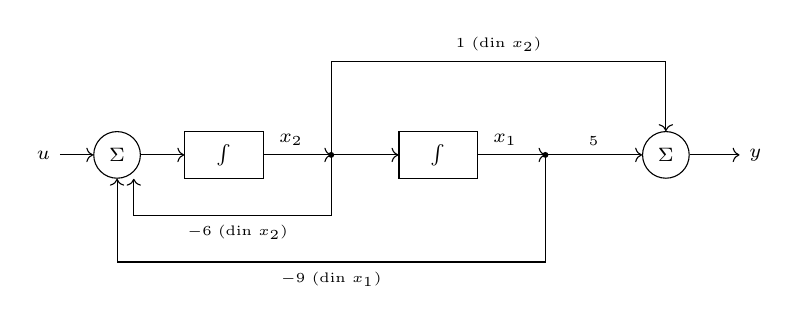
\begin{tikzpicture}[scale=0.85, every node/.style={font=\scriptsize}]
\node (u) at (0,0) {$u$};
\node[draw,circle,minimum size=0.5cm] (s1) at (1.1,0) {$\Sigma$};
\draw[->] (u)--(s1);
\node[draw,minimum width=1cm,minimum height=0.6cm] (i1) at (2.7,0) {$\int$};
\draw[->] (s1)--(i1);
\coordinate (a) at (4.3,0);
\draw[->] (i1) -- (a) node[above,pos=0.4]{$x_2$};
\filldraw (a) circle (1pt);
\node[draw,minimum width=1cm,minimum height=0.6cm] (i2) at (5.9,0) {$\int$};
\draw[->] (a) -- (i2);
\coordinate (b) at (7.5,0);
\draw[->] (i2) -- (b) node[above,pos=0.4]{$x_1$};
\filldraw (b) circle (1pt);
\node[draw,circle,minimum size=0.5cm] (sy) at (9.3,0) {$\Sigma$};
\draw[->] (b) -- (sy) node[midway,above]{\tiny $5$};
\draw[->] (a) -- ++(0,1.4) -| (sy.north);
\node[above] at (6.8,1.4){\tiny $1$ (din $x_2$)};
\draw[->] (sy) -- (10.4,0) node[right]{$y$};
\draw[->] (b) -- ++(0,-1.6) -| (s1.south);
\node[below] at (4.3,-1.6){\tiny $-9$ (din $x_1$)};
\draw[->] (a) -- ++(0,-0.9) -| ($(s1.south)+(0.25,0)$);
\node[below] at (2.9,-0.9){\tiny $-6$ (din $x_2$)};
\end{tikzpicture}
\tip{\textit{Notă:} nu există un al doilea sumator între cele două integratoare — $\dot x_1{=}x_2$ e o integrare directă, fără alți termeni; toate reacțiile ($-9x_1$, $-6x_2$) intră o singură dată, la primul sumator.}
\end{center}

\textbf{Subiect 2 — Bode + eroare staționară pentru $G(s)=5\dfrac{0{,}1s+1}{s}$ (reacție unitară):} rezolvare pas cu pas, cu formula generală înainte de fiecare aplicare numerică. (Identic cu Subiectul B din \hyperref[sec:21]{secțiunea 21}, biletul reluare toamnă 2025.)

\textbf{Pasul 1 — forma generală:} orice sistem cu un integrator și un singur zero de ordinul 1 se scrie $G(j\omega)=\dfrac{K(1+j\omega T)}{j\omega}$, produs a trei factori de bază (\hyperref[sec:7]{secțiunea 7}): $K$ (câștig), $1/(j\omega)$ (integrator), $(1+j\omega T)$ (zero).

\textit{Aplicare:} $G(j\omega)=5\dfrac{1+0{,}1j\omega}{j\omega}\Rightarrow K{=}5,\ T{=}0{,}1$.

\textbf{Pasul 2 — frecvența de frângere:} formula generală $\omega_f=1/T$. \textit{Aplicare:} $\omega_f=1/0{,}1=10$rad/s — singura din tot sistemul ($K$ și integratorul nu au una).

\textbf{Pasul 3 — formula exactă} (aceeași care dă curba „exact" din grafic), din $G(j\omega)=\dfrac{K(1+j\omega T)}{j\omega}$:
\begin{keyeq}\color{red!65!black}
$$|G(j\omega)|_{dB}=20\lg K+20\lg\sqrt{1+(\omega T)^2}-20\lg\omega,\qquad \varphi(\omega)=-90^\circ+\mathrm{arctg}(\omega T)$$
\end{keyeq}
\textit{Aplicare} ($K{=}5,T{=}0{,}1$): $|G(j\omega)|_{dB}=20\lg5+20\lg\sqrt{1+(0{,}1\omega)^2}-20\lg\omega$,\quad $\varphi(\omega)=-90^\circ+\mathrm{arctg}(0{,}1\omega)$.

\textbf{Pasul 4 — regulile asimptotice generale pentru fiecare factor} (\hyperref[sec:7]{secțiunea 7}), aplicate imediat pentru $K{=}5,\,\omega_f{=}10$:
\begin{center}
\footnotesize
\begin{tabular}{|p{2.5cm}|p{6.6cm}|p{6.9cm}|}
\hline
\textbf{Factor} & \textbf{Modul (formulă generală $\to$ aplicat)} & \textbf{Fază (formulă generală $\to$ aplicat)} \\\hline
$K$ & orizontală, $K_{dB}{=}20\lg|K|$ $\to$ $20\lg5\approx14$dB & $0^\circ$ dacă $K{>}0$, $180^\circ$ dacă $K{<}0$ $\to$ $0^\circ$ \\\hline
$1/(j\omega)$ & pantă $-20$dB/dec, prin $0$dB la $\omega{=}1$ (nu depinde de $K$) & $-90^\circ$ constant $\to$ $-90^\circ$ \\\hline
$(1{+}j\omega T)$ & $0$dB sub $\omega_f{=}1/T$; pantă $+20$dB/dec peste $\to$ sub $10$: $0$dB; peste $10$: $+20$dB/dec & $0^\circ$ sub $\omega_f/10$; $+90^\circ$ peste $10\omega_f$; $+45^\circ$ la $\omega_f$ $\to$ $0^\circ$ la $1$; $+90^\circ$ la $100$; $+45^\circ$ la $10$ \\\hline
\end{tabular}
\end{center}

\textbf{Pasul 5 — le însumez} (regula de aur: dB-ii se adună, gradele se adună):

\textit{Modul:} sub $\omega_f$, formula generală a dreptei compuse $K$+integrator e $20\lg K-20\lg\omega$, care taie $0$dB la $\omega_0=K$ (rezolvi $20\lg K=20\lg\omega_0$). \textit{Aplicare:} $\omega_0{=}5$. Peste $\omega_f$, panta compusă devine $-20{+}20{=}0$dB/dec (orizontală), la nivelul general $20\lg(K/\omega_f)$. \textit{Aplicare:} $20\lg(5/10){=}20\lg0{,}5\approx-6$dB.

\textit{Fază:} formula generală asimptotică (3 drepte) e $-90^\circ$ sub $\omega_f/10$, apoi crește liniar cu $+45^\circ$/decadă până la $10\omega_f$, unde ajunge la $0^\circ$. \textit{Aplicare:} $-90^\circ$ sub $\omega{=}1$; la $\omega{=}10$ (chiar $\omega_f$) $-90{+}45{=}-45^\circ$; la $\omega{=}100$ atinge $0^\circ$.

\textbf{Pasul 6 — desenez efectiv, cu rigla, pe foaie} (algoritmul \hyperref[sec:8]{secțiunii 8}):

\textit{Pregătesc axele.} N-ai hârtie logaritmică la examen, deci axa orizontală ($\omega$) o construiești manual: marchezi puncte \textbf{egal distanțate} pentru fiecare \textbf{putere a lui 10}: $0{,}1-1-10-100-1000$. Distanța dintre oricare doi vecini e \textbf{aceeași} pe hârtie (asta e toată ideea scării log — fiecare pas la dreapta înmulțește $\omega$ cu $10$, nu adaugă un număr fix). Axa verticală: dB pentru modul, grade pentru fază.

\textit{Modul — rețetă mecanică:}
\begin{enumerate}
\item Pui un punct la $\omega{=}1$, înălțime $K_{dB}{=}14$dB (calculat la Pasul 4).
\item Din acel punct, tragi o linie dreaptă cu panta $-20$dB/decadă: mecanic, \textbf{la fiecare diviziune spre dreapta cobori cu 20}, la fiecare diviziune spre stânga urci cu 20. Deci la $\omega{=}0{,}1$ ești la $14{+}20{=}34$dB; continuând spre dreapta, la $\omega{=}10$ ai fi la $14{-}20{=}{-}6$dB.
\item \textbf{Te oprești din tras linia asta exact la $\omega_f{=}10$} — acolo intervine zero-ul (Pasul 2). De la $\omega{=}10$ încolo, schimbi panta la $0$dB/decadă (linie \textbf{orizontală}), pornind chiar de la valoarea unde ai ajuns, $-6$dB.
\item Asta e toată asimptota: coboară în linie dreaptă până la $\omega{=}10$, apoi devine plată la $-6$dB.
\item (Pentru curba exactă, albastră: rotunjești ușor colțul de la $\omega_f$, trecând cu $\approx3$dB sub asimptotă acolo — o singură frecvență de frângere de ordin 1 dă eroarea maximă de $3$dB exact în colț, vezi \hyperref[sec:7]{secțiunea 7}.)
\end{enumerate}

\textit{Fază — rețetă mecanică:}
\begin{enumerate}
\item Marchezi $\omega_f/10{=}1$ și $10\omega_f{=}100$ pe aceeași axă orizontală (le ai deja ca diviziuni).
\item Sub $\omega{=}1$: linie orizontală la $-90^\circ$.
\item Între $\omega{=}1$ și $\omega{=}100$ (exact $2$ decade): tragi o linie dreaptă de la punctul $({-}90^\circ$ la $\omega{=}1)$ până la punctul $(0^\circ$ la $\omega{=}100)$ — o urcare de $90^\circ$ pe $2$ decade, adică pantă $45^\circ$/decadă.
\item Peste $\omega{=}100$: linie orizontală la $0^\circ$.
\item \tip{\textbf{Control:} la $\omega_f{=}10$ (mijlocul segmentului înclinat, o decadă din fiecare parte) trebuie să treci exact prin $-45^\circ$ — dacă nu, ai greșit panta.}
\end{enumerate}

Rezultatul (curbe exacte cu albastru, asimptote cu roșu) e graficul de mai jos.

\textbf{Pasul 7 — eroare staționară} (formule generale $K_p,K_v$ — \hyperref[sec:18]{secțiunea 18}; tip $1$, un singur integrator): $K_p{=}\lim_{s\to0}G(s){=}\infty$, $K_v{=}\lim_{s\to0}sG(s){=}5$:
\begin{keyeq}\color{red!65!black}
$$e_{ss}(\text{treaptă})=0,\qquad e_{ss}(\text{rampă})=1/K_v=0{,}2$$
\end{keyeq}

\begin{center}
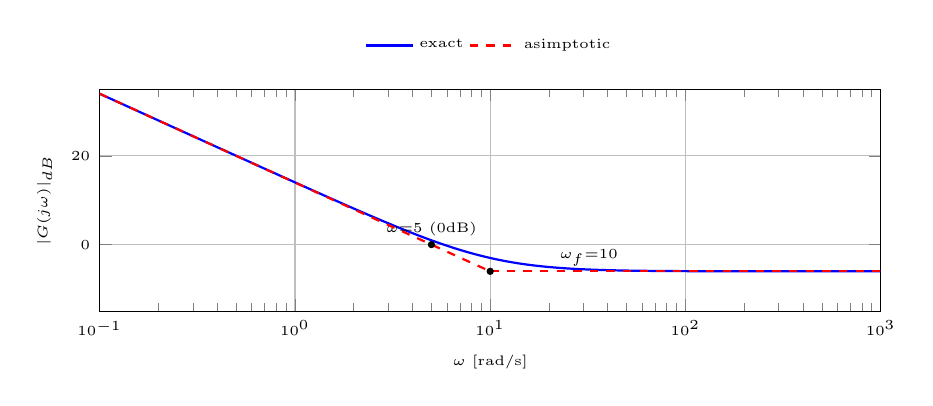
\begin{tikzpicture}
\begin{semilogxaxis}[
    width=11.5cm, height=4.4cm,
    xlabel={\tiny $\omega$ [rad/s]}, ylabel={\tiny $|G(j\omega)|_{dB}$},
    xmin=0.1, xmax=1000, ymin=-15, ymax=35,
    grid=major, tick label style={font=\tiny},
    legend style={font=\tiny,at={(0.5,1.28)},anchor=north,legend columns=2,draw=none}
]
\addplot[domain=0.1:1000,samples=200,blue,thick] {20*ln(5*sqrt(1+(0.1*x)^2)/x)/ln(10)};
\addplot[domain=0.1:10,samples=2,red,thick,dashed] {20*ln(5/x)/ln(10)};
\addplot[domain=10:1000,samples=2,red,thick,dashed] {20*ln(0.5)/ln(10)};
\addplot[only marks,mark=*,mark size=1.1pt,black] coordinates {(5,0)(10,-6.02)};
\node[font=\tiny] at (axis cs:5,3.5) {$\omega{=}5$ (0dB)};
\node[font=\tiny] at (axis cs:32,-3) {$\omega_f{=}10$};
\legend{exact,asimptotic}
\end{semilogxaxis}
\end{tikzpicture}

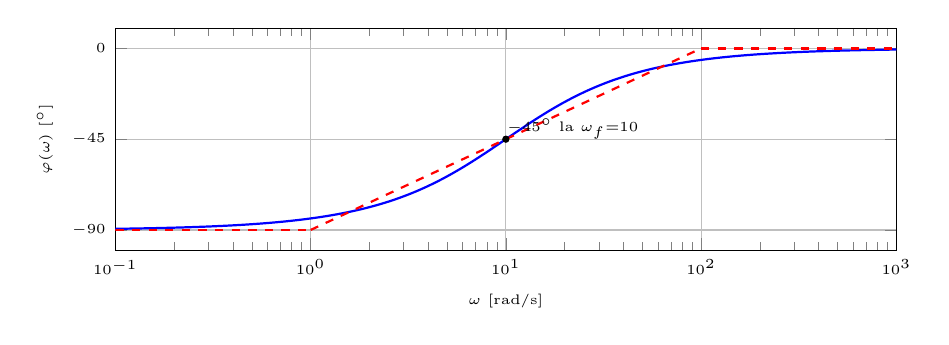
\begin{tikzpicture}
\begin{semilogxaxis}[
    width=11.5cm, height=4.4cm,
    xlabel={\tiny $\omega$ [rad/s]}, ylabel={\tiny $\varphi(\omega)\ [^\circ]$},
    xmin=0.1, xmax=1000, ymin=-100, ymax=10,
    ytick={-90,-45,0}, grid=major, tick label style={font=\tiny}
]
\addplot[domain=0.1:1000,samples=200,blue,thick] {-90+atan(0.1*x)};
\addplot[domain=0.1:1,samples=2,red,thick,dashed] {-90};
\addplot[domain=1:100,samples=2,red,thick,dashed] {-90+45*ln(x)/ln(10)};
\addplot[domain=100:1000,samples=2,red,thick,dashed] {0};
\addplot[only marks,mark=*,mark size=1.1pt,black] coordinates {(10,-45)};
\node[font=\tiny] at (axis cs:22,-40) {$-45^\circ$ la $\omega_f{=}10$};
\end{semilogxaxis}
\end{tikzpicture}
\end{center}
\tip{\textit{Observație grafic:} sub $\omega{=}10$ modulul scade cu $-20$dB/dec (linia dreaptă e exactă — vine doar de la integrator, factorul $(0{,}1s{+}1)$ e încă $\approx1$ acolo); peste $\omega{=}10$ panta devine $0$dB/dec (cele două pante, $-20$ și $+20$, se anulează). Faza pleacă din $-90^\circ$ (integrator pur) și urcă spre $0^\circ$, trecând prin $-45^\circ$ exact la frecvența de frângere $\omega_f{=}10$ — curba exactă (albastru) și asimptota în 3 drepte (roșu) diferă cel mai mult tot acolo.}

\textbf{Subiect 3 — reacție NEunitară: $G(s)=\dfrac{k}{s(s+2)}$, $H(s)=\dfrac1{s+4}$:}

\textbf{a) Stabilitate prin curbă polară:} se lucrează cu funcția de transfer de pe calea directă$\times$reacție (tip 1, $P{=}0$ — deschis stabil, formă simplificată \hyperref[sec:10]{secțiunea 10}):
\begin{keyeq}\color{red!65!black}
$$L(s)=G(s)H(s)=\dfrac{k}{s(s+2)(s+4)}$$
\end{keyeq}

\textit{Raționalizarea, pas cu pas} (tehnica generală, \hyperref[sec:9]{secțiunea 9}): pun $s=j\omega$ și mai întâi aduc numitorul la forma $A+jB$, ca să știu ce conjugată să folosesc. Înmulțesc întâi doi din cei trei factori:
$$(j\omega+2)(j\omega+4)=(j\omega)^2+6j\omega+8=-\omega^2+6j\omega+8=(8-\omega^2)+6j\omega$$
apoi înmulțesc cu al treilea factor, $j\omega$ (atenție: $j\cdot j={-}1$):
$$j\omega\big[(8-\omega^2)+6j\omega\big]=j\omega(8-\omega^2)+6j^2\omega^2=\underbrace{-6\omega^2}_{A}+\underbrace{j\,\omega(8-\omega^2)}_{jB}$$
Deci numitorul lui $L(j\omega)$ e $A+jB$, cu $A={-}6\omega^2$ și $B=\omega(8{-}\omega^2)$, deci $L(j\omega)=\dfrac{k}{-6\omega^2+j\,\omega(8-\omega^2)}$. Înmulțesc sus și jos cu conjugata numitorului, $A-jB$ (trucul standard: $(A{+}jB)(A{-}jB)=A^2{+}B^2$, un număr REAL, deci dispare $j$-ul de la numitor):
$$L(j\omega)=\dfrac{k(A-jB)}{(A+jB)(A-jB)}=\dfrac{k\big[-6\omega^2-j\,\omega(8-\omega^2)\big]}{(-6\omega^2)^2+\big[\omega(8-\omega^2)\big]^2}=\dfrac{-6k\omega^2-jk\,\omega(8-\omega^2)}{\omega^2\big[36\omega^2+(8-\omega^2)^2\big]}$$
(la numitor am scos $\omega^2$ factor comun din $36\omega^4+\omega^2(8{-}\omega^2)^2$). Despart partea reală (fără $j$) de partea imaginară (cu $j$), simplificând câte un $\omega$ unde se poate — asta sunt formulele finale pe care le folosesc mai departe:
\begin{keyeq}\color{red!65!black}
$$\mathrm{Re}\{L(j\omega)\}=\dfrac{-6k}{36\omega^2+(8-\omega^2)^2},\qquad \mathrm{Im}\{L(j\omega)\}=\dfrac{-k(8-\omega^2)}{\omega\big[36\omega^2+(8-\omega^2)^2\big]}$$
\end{keyeq}

Curba taie axa reală acolo unde $\mathrm{Im}\{L(j\omega)\}=0$ (asta e chiar condiția — un punct e „pe axa reală" exact când n-are parte imaginară). Pun numărătorul lui $\mathrm{Im}\{L(j\omega)\}$ egal cu zero (numitorul $\omega[36\omega^2{+}(8{-}\omega^2)^2]$ nu se anulează pentru $\omega\ne0$, fiind o sumă de termeni pozitivi):
$$-k(8-\omega^2)=0\ \overset{k\ne0}{\Longrightarrow}\ 8-\omega^2=0\ \Rightarrow\ \omega^2=8\ \Rightarrow\ \omega=2\sqrt2\approx2{,}83\text{ rad/s}\quad(\omega{>}0,\text{ soluția fizică})$$
Înlocuiesc apoi această valoare înapoi în $\mathrm{Re}\{L(j\omega)\}$ ca să aflu UNDE anume taie axa (la $\omega^2{=}8$: $36\omega^2{=}288$ și $(8{-}\omega^2)^2{=}0$):
$$\mathrm{Re}\{L(j2\sqrt2)\}=\dfrac{-6k}{288+0}=-\dfrac{k}{48}$$

\textit{Cum desenez efectiv curba, pe hârtie} (folosind regulile de comportament la capete, \hyperref[sec:9]{secțiunea 9}): la $\omega\to0^+$ (tip $1$ — un singur pol în origine, la numitor factorul $s$), calculez limita lui $\mathrm{Re}$ direct din formula de mai sus (aici NU dă $0/0$, deci pot pune direct $\omega{=}0$): $\lim_{\omega\to0}\mathrm{Re}\{L(j\omega)\}=\dfrac{-6k}{0+64}=-\dfrac{3k}{32}$. Partea imaginară însă tinde la $-\infty$ (numărătorul $-k(8-\omega^2)\to-8k$ rămâne finit, dar numitorul $\omega[\cdots]\to0$). Deci curba are o asimptotă verticală la $\mathrm{Re}=-3k/32$, pe care coboară spre $-\infty$ când $\omega\to0^+$ — asta explică regula generală „tip 1 $\Rightarrow$ asimptotă paralelă cu semiaxa imaginară negativă", dar acum știi și UNDE anume (poziția pe orizontală).

La $\omega\to\infty$: modulul $\to0$ (numărătorul, o constantă $k$, crește mult mai încet decât numitorul, de gradul 3) $\Rightarrow$ curba se apropie de origine, tangentă la semiaxa imaginară pozitivă, în sens orar (regula generală pentru $n{-}m{=}3$, \hyperref[sec:9]{secțiunea 9}).

Puncte de control intermediare (calculate din formulele Re/Im de mai sus, pentru $k{=}10$ ca reper — aceeași valoare folosită și în desenul de mai jos și la exemplul de la b); pentru alt $k$ înmulțești toate valorile cu $k/10$):
\begin{itemize}
\item $\omega{=}1$: $\mathrm{Re}\approx-0{,}706$, $\mathrm{Im}\approx-0{,}824$ (cadranul III)
\item $\omega{=}2{,}83$: $\mathrm{Re}{=}-10/48\approx-0{,}208$, $\mathrm{Im}{=}0$ (pe axa reală)
\item $\omega{=}5$: $\mathrm{Re}\approx-0{,}050$, $\mathrm{Im}\approx+0{,}029$ (cadranul II)
\end{itemize}
Cum unesc punctele: pornesc de jos, de pe asimptota verticală ($\omega\to0^+$), urc prin cadranul III, trec prin axa reală exact la $\omega{=}2{,}83$ (punctul calculat mai sus), continui prin cadranul II, și mă apropii de origine tangent la semiaxa Im pozitivă — o singură curbă continuă, fără colțuri, parcursă mereu în sensul crescător al lui $\omega$ (asta e desenul de mai jos).

\textit{De ce merge așa (pe scurt):} faza scade constant, $-90^\circ\to-270^\circ$ — vectorul se rotește tot timpul în același sens (orar), niciodată invers. Modulul scade constant, $\infty\to0$. Deci e o spirală care se strânge orar spre origine; taie axa reală o singură dată, exact când faza trece prin $-180^\circ$ (acolo e $-k/48$). Mica „buclă" de lângă origine e obligatorie — vine din regula de la capăt (tangent la Im$^+$, nu la axa reală).

Curba nu încercuiește $-1$ $\iff k/48<1$:
\begin{keyeq}\color{red!65!black}
$$0<k<48\qquad\text{(verificat identic prin Routh pe }s^3{+}6s^2{+}8s{+}k{=}0\text{)}$$
\end{keyeq}

\textit{Desenul cerut la a)} (curba polară, desenată \textbf{la scară reală} din puncte calculate — pentru $k{=}10$ ca reper numeric; pentru alt $k$ toate coordonatele se scalează proporțional):
\begin{center}
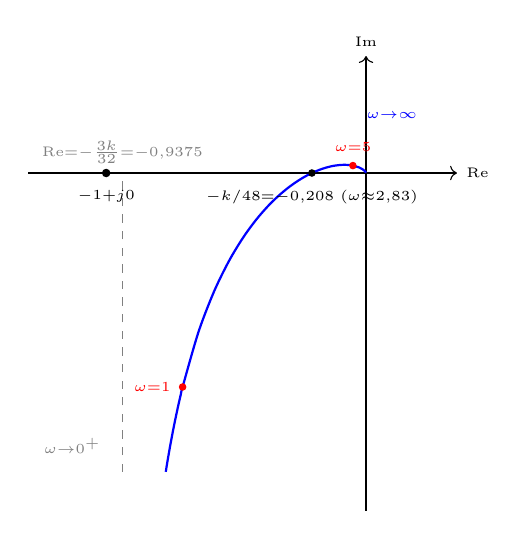
\begin{tikzpicture}[scale=3.3]
\draw[->] (-1.3,0) -- (0.35,0) node[right]{\tiny Re};
\draw[->] (0,-1.3) -- (0,0.45) node[above]{\tiny Im};
\draw[dashed,gray] (-0.9375,-1.15) -- (-0.9375,0);
\node[gray,font=\tiny] at (-0.9375,0.08) {$\mathrm{Re}{=}{-}\tfrac{3k}{32}{=}{-}0{,}9375$};
\node[gray,font=\tiny] at (-1.13,-1.05) {$\omega{\to}0^+$};
\draw[thick,blue] plot[smooth] coordinates {
(-0.7707,-1.15) (-0.765,-1.1148) (-0.7592,-1.0808) (-0.7534,-1.0481) (-0.7475,-1.0165) (-0.7417,-0.986) (-0.7358,-0.9566) (-0.7298,-0.9282) (-0.7239,-0.9007) (-0.7179,-0.8741) (-0.7119,-0.8484) (-0.7059,-0.8235) (-0.6448,-0.6119) (-0.5845,-0.4551) (-0.5265,-0.3369) (-0.472,-0.247) (-0.4216,-0.1783) (-0.3757,-0.1257) (-0.3342,-0.0855) (-0.297,-0.0547) (-0.2638,-0.0312) (-0.2344,-0.0134) (-0.2083,0.0) (-0.1813,0.0115) (-0.158,0.0195) (-0.138,0.0249) (-0.1207,0.0283) (-0.1058,0.0303) (-0.093,0.0313) (-0.0819,0.0315) (-0.0723,0.0312) (-0.064,0.0306) (-0.0567,0.0297) (-0.0505,0.0286) (-0.0266,0.0215) (-0.0151,0.0156) (-0.0091,0.0113) (-0.0057,0.0084) (-0.0038,0.0063) (-0.0026,0.0049) (-0.0018,0.0038) (-0.0013,0.003) (-0.001,0.0024) (-0.0007,0.002) (-0.0006,0.0017) (-0.0005,0.0014) (-0.0004,0.0012)
};
\node[blue,font=\tiny] at (0.1,0.22) {$\omega{\to}\infty$};
\filldraw (-1,0) circle (0.4pt); \node[below,font=\tiny] at (-1,-0.03){$-1{+}j0$};
\filldraw (-0.2083,0) circle (0.35pt); \node[below,font=\tiny] at (-0.2083,-0.03){$-k/48{=}{-}0{,}208$ ($\omega{\approx}2{,}83$)};
\filldraw[red] (-0.7059,-0.8235) circle (0.35pt); \node[red,left,font=\tiny] at (-0.715,-0.8235){$\omega{=}1$};
\filldraw[red] (-0.0505,0.0286) circle (0.35pt); \node[red,above,font=\tiny] at (-0.05,0.045){$\omega{=}5$};
\end{tikzpicture}
\end{center}
\tip{Desen la scară reală pentru $k{=}10$ — punctele au fost calculate direct din formulele $\mathrm{Re}\{L(j\omega)\},\mathrm{Im}\{L(j\omega)\}$ de mai sus (nu aproximate din ochi). Curba taie axa reală o singură dată, la $-k/48$: cât timp acel punct e la \textbf{dreapta} lui $-1$ (adică $k{<}48$), curba nu încercuiește punctul critic $\Rightarrow$ sistem stabil în circuit închis. Pentru alt $k$ decât $10$, forma rămâne identică (aceeași spirală) — doar coordonatele se înmulțesc cu $k/10$. Diagrama de la b) (mai jos) e aceeași curbă, cu cercul unitate adăugat ca să se vadă și marginea de fază.}

\textbf{b) Marginea de fază} (formula generală, \hyperref[sec:11]{secțiunea 11}: $\omega_t$ = pulsația de tăiere, $|L(j\omega_t)|{=}1$; $\gamma{=}180^\circ{+}\angle L(j\omega_t)$). Exemplu ilustrativ pt. $k{=}10\in(0,48)$ — pentru $k$ din enunțul tău repetă identic: $|L(j\omega_t)|{=}1\Rightarrow\omega_t\sqrt{(\omega_t^2{+}4)(\omega_t^2{+}16)}{=}10\Rightarrow\omega_t\approx1{,}065$rad/s. $\angle L(j\omega_t){=}{-}90^\circ{-}\mathrm{arctg}\tfrac{\omega_t}2{-}\mathrm{arctg}\tfrac{\omega_t}4\approx-132{,}9^\circ$:
\begin{keyeq}\color{red!65!black}
$$\gamma=180^\circ+\angle L(j\omega_t)\approx\mathbf{47{,}1^\circ}$$
\end{keyeq}

\tip{\textit{Clarificare — de ce $\sqrt{\omega^2{+}4}$ și nu $(\omega{+}2)^2$:} $|L(j\omega)|$ e un \textbf{modul de număr complex}, nu pătratul unui binom real. Factorul $(s{+}2)$ evaluat în $s{=}j\omega$ devine numărul complex $j\omega{+}2$ (parte reală $2$, parte imaginară $\omega$), iar modulul lui e $|j\omega{+}2|{=}\sqrt{2^2{+}\omega^2}{=}\sqrt{\omega^2{+}4}$ — regula $|a{+}jb|{=}\sqrt{a^2{+}b^2}$, NU $(a{+}b)^2$. Dacă ai calcula $(\omega{+}2)^2{=}\omega^2{+}4\omega{+}4$, ai trata greșit $j\omega$ ca pe un termen real obișnuit care se adună cu $2$, deși el stă pe axa imaginară — de-asta lipsește termenul $4\omega$, iar cel corect e doar $\omega^2{+}4$. Analog, $(s{+}4)\to j\omega{+}4$ dă $\sqrt{\omega^2{+}16}$, nu $(\omega{+}4)^2$.}

\tip{\textit{Clarificare — de unde vine $10$ și dacă e $k$:} da, $10$ e chiar valoarea aleasă pentru $k$ în acest exemplu (orice $k\in(0,48)$, intervalul găsit la a), ar merge la fel — am ales $10$ doar ca să am o cifră concretă). Ecuația de definiție a pulsației de tăiere e $|L(j\omega_t)|{=}1$, adică $\dfrac{k}{\omega_t\sqrt{(\omega_t^2{+}4)(\omega_t^2{+}16)}}{=}1\ \Leftrightarrow\ \omega_t\sqrt{(\omega_t^2{+}4)(\omega_t^2{+}16)}{=}k$. Când pun $k{=}10$, membrul drept devine $10$ — acel $10$ nu e un rezultat calculat separat, e pur și simplu $k$ înlocuit numeric. Dacă la subiectul tău $k$ nu are o valoare dată explicit la 3b), fără un $k$ numeric nu obții un $\omega_t$ numeric, deci nici un $\gamma$ numeric — răspunsul rămâne simbolic în funcție de $k$, sau folosești un $k$ de reper (ca $10$) ca să ilustrezi metoda.}

\textit{Cum aflu efectiv $\omega_t$ — calculul detaliat} (pornesc de la ecuația de mai sus, $\omega_t\sqrt{(\omega_t^2{+}4)(\omega_t^2{+}16)}{=}k$, cu $k{=}10$):

\textbf{Pasul 1 — scap de radical, ridicând la pătrat ambii membri} (pot face asta fără riscul de a introduce soluții străine, pentru că ambii membri sunt deja pozitivi — $\omega_t{>}0$ și $k{>}0$):
$$\omega_t^2(\omega_t^2{+}4)(\omega_t^2{+}16)=k^2$$

\textbf{Pasul 2 — notez $x{=}\omega_t^2$} (asta transformă ecuația într-una polinomială „normală", de gradul 3 în $x$, în loc de gradul 6 în $\omega_t$; observă că $x{>}0$ obligatoriu, fiindcă $x$ e un pătrat):
$$x(x{+}4)(x{+}16)=k^2$$

\textbf{Pasul 3 — desfac parantezele} (înmulțesc întâi $(x{+}4)(x{+}16){=}x^2{+}20x{+}64$, apoi cu $x$):
\begin{keyeq}\color{red!65!black}
$$x^3+20x^2+64x-k^2=0\ \overset{k=10}{\Longrightarrow}\ x^3+20x^2+64x-100=0$$
\end{keyeq}

\tip{Nu există rădăcină „frumoasă" (întreagă/rațională) aici — dacă încerci teorema rădăcinii raționale (candidați: divizorii lui $100$, adică $\pm1,\pm2,\pm4,\pm5,\pm10,\ldots$), niciunul nu anulează polinomul. E normal: coeficienții $4$ și $16$ vin din pătratele pulsațiilor de frângere ($2^2$ și $4^2$), care rar dau o ecuație cu rădăcini întregi. Deci se rezolvă \textbf{numeric} — la examen, fie cu calculatorul (mod ecuație/solve, dacă e permis), fie prin încercări succesive (metoda de mai jos), fie citind aproximativ de pe diagrama Bode asimptotică și rafinând.}

\textbf{Pasul 4 — rezolv numeric prin încercări (bisecție/Newton pe scurt)}, căutând rădăcina pozitivă a lui $f(x){=}x^3{+}20x^2{+}64x{-}100$:
\begin{itemize}
\item $f(1)=1{+}20{+}64{-}100={-}15$ (negativ)
\item $f(1{,}2)=1{,}728{+}28{,}8{+}76{,}8{-}100={+}7{,}33$ (pozitiv) $\Rightarrow$ rădăcina e între $1$ și $1{,}2$
\item $f(1{,}14)=1{,}48{+}25{,}99{+}72{,}96{-}100={+}0{,}43$; $f(1{,}13)=1{,}44{+}25{,}54{+}72{,}32{-}100={-}0{,}70$ $\Rightarrow$ între $1{,}13$ și $1{,}14$
\item rafinez încă un pas $\Rightarrow x\approx1{,}136$
\end{itemize}
(Alternativ, mai rapid: metoda Newton, $x_{n+1}{=}x_n{-}f(x_n)/f'(x_n)$ cu $f'(x){=}3x^2{+}40x{+}64$; pornind din $x_0{=}1$ converge la $x\approx1{,}136$ în 2 pași — aceeași valoare, doar ajungi acolo mai repede.)

\textbf{Pasul 5 — revin la $\omega_t$} (nu uita substituția $x{=}\omega_t^2$, deci trebuie să extragi radical, nu să folosești $x$ direct):
\begin{keyeq}\color{red!65!black}
$$\omega_t=\sqrt{x}\approx\sqrt{1{,}136}\approx\mathbf{1{,}065\ rad/s}$$
\end{keyeq}
\tip{Greșeala tipică aici e să uiți Pasul 5 și să raportezi $\omega_t{=}1{,}136$ (asta e $\omega_t^2$, nu $\omega_t$!) — verifică mereu dimensional: $x$ avea unități de rad$^2$/s$^2$, $\omega_t$ trebuie să fie în rad/s.}

\textit{Cum se vede $\gamma$ direct pe caracteristica polară} (aceeași curbă $L(j\omega)$ ca la a), acum la scară reală pentru $k{=}10$, cu cercul de rază $1$ desenat explicit): punctul unde curba taie cercul unitate ($|L(j\omega_t)|{=}1$) e chiar $\omega_t$; unghiul dintre semiaxa reală negativă (direcția spre $-1{+}j0$) și vectorul $\overrightarrow{OL(j\omega_t)}$, măsurat de la $-1$ spre curbă, este \textbf{exact marginea de fază $\gamma$} — geometric, „cât mai trebuie rotită curba (spre $-1$) ca să treacă exact prin $-1$".

\begin{center}
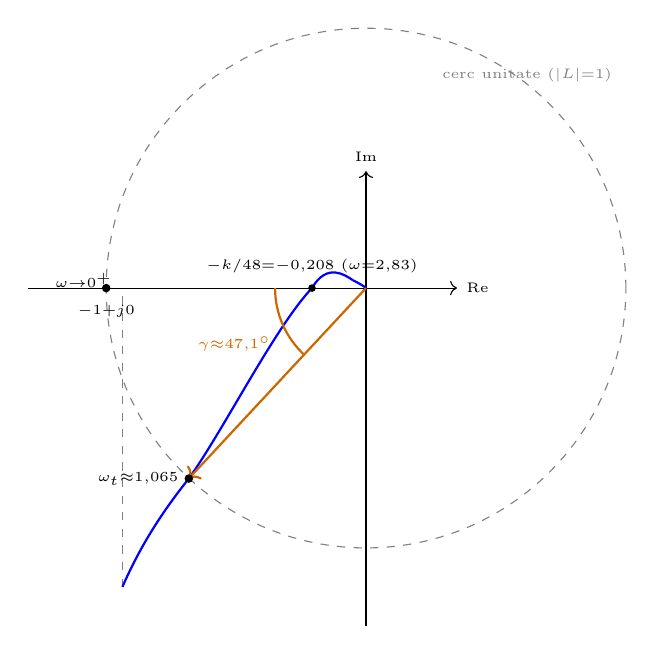
\begin{tikzpicture}[scale=3.3]
\draw[->] (-1.3,0) -- (0.35,0) node[right]{\tiny Re};
\draw[->] (0,-1.3) -- (0,0.45) node[above]{\tiny Im};
\draw[dashed,gray] (0,0) circle (1);
\node[gray,font=\tiny] at (0.62,0.82) {cerc unitate ($|L|{=}1$)};
\draw[dashed,gray] (-0.9375,-1.15) -- (-0.9375,0);
\draw[thick,blue] (-0.9375,-1.15) .. controls (-0.85,-0.95) and (-0.75,-0.82) .. (-0.682,-0.733);
\draw[thick,blue] (-0.682,-0.733) .. controls (-0.55,-0.55) and (-0.35,-0.15) .. (-0.208,0);
\draw[thick,blue] (-0.208,0) .. controls (-0.15,0.1) and (-0.08,0.05) .. (-0.05,0.03);
\draw[thick,blue] (-0.05,0.03) .. controls (-0.02,0.015) and (-0.005,0.005) .. (0,0);
\draw[->,thick,orange!80!black] (0,0) -- (-0.682,-0.733);
\draw[thick,orange!80!black] (180:0.35) arc (180:227.1:0.35);
\node[orange!80!black,font=\tiny] at (203:0.55) {$\gamma{\approx}47{,}1^\circ$};
\filldraw (-1,0) circle (0.4pt); \node[below,font=\tiny] at (-1,-0.03){$-1{+}j0$};
\filldraw (-0.208,0) circle (0.35pt); \node[above,font=\tiny] at (-0.208,0.02){$-k/48{=}{-}0{,}208$ ($\omega{=}2{,}83$)};
\filldraw (-0.682,-0.733) circle (0.4pt); \node[left,font=\tiny] at (-0.685,-0.735){$\omega_t{\approx}1{,}065$};
\node[left,font=\tiny] at (-0.94,0.03){$\omega{\to}0^+$};
\end{tikzpicture}
\end{center}
\tip{\textit{Observație grafic:} $-1{+}j0$ e la $180^\circ$; punctul de tăiere $\omega_t$ e la unghiul $\angle L(j\omega_t){\approx}{-}132{,}9^\circ$ (adică $227{,}1^\circ$ măsurat pozitiv). Distanța unghiulară dintre ele, $227{,}1^\circ{-}180^\circ{=}47{,}1^\circ$, e chiar $\gamma$ — vizual, cu cât e mai „departe" (unghiular) punctul $\omega_t$ de $-1$, cu atât sistemul are mai multă rezervă de stabilitate. Dacă $\omega_t$ ar ajunge chiar pe axa reală negativă (suprapus peste $-1$), $\gamma{=}0$ și sistemul ar fi la limita de stabilitate — exact cazul $k{=}48$ de la a).}

\begin{center}
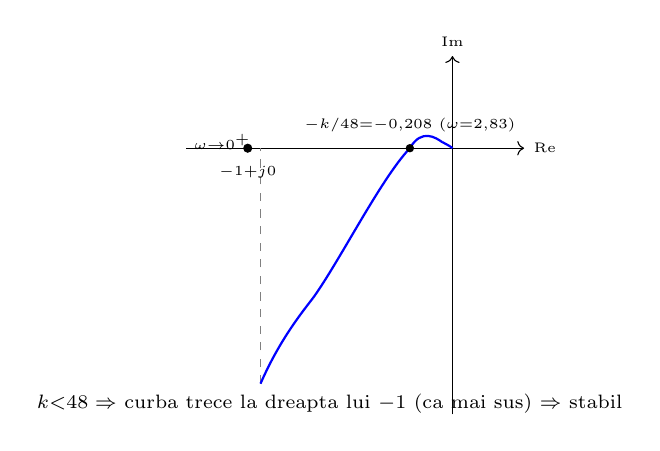
\begin{tikzpicture}[scale=2.6]
\draw[->] (-1.3,0) -- (0.35,0) node[right]{\tiny Re};
\draw[->] (0,-1.3) -- (0,0.45) node[above]{\tiny Im};
\draw[dashed,gray] (-0.9375,-1.15) -- (-0.9375,0);
\node[left,font=\tiny] at (-0.9375,0.03){$\omega{\to}0^+$};
\draw[thick,blue] (-0.9375,-1.15) .. controls (-0.85,-0.95) and (-0.75,-0.82) .. (-0.682,-0.733);
\draw[thick,blue] (-0.682,-0.733) .. controls (-0.55,-0.55) and (-0.35,-0.15) .. (-0.208,0);
\draw[thick,blue] (-0.208,0) .. controls (-0.15,0.1) and (-0.08,0.05) .. (-0.05,0.03);
\draw[thick,blue] (-0.05,0.03) .. controls (-0.02,0.015) and (-0.005,0.005) .. (0,0);
\filldraw (-0.208,0) circle (0.5pt); \node[above,font=\tiny] at (-0.208,0.03){$-k/48{=}{-}0{,}208$ ($\omega{=}2{,}83$)};
\filldraw (-1,0) circle (0.55pt); \node[below,font=\tiny] at (-1,-0.04){$-1{+}j0$};
\node[align=center,font=\scriptsize] at (-0.6,-1.25){$k{<}48\Rightarrow$ curba trece la dreapta lui $-1$ (ca mai sus) $\Rightarrow$ stabil};
\end{tikzpicture}
\end{center}

\textit{Verificare prin Bode a marginii de fază} (aceeași $L(j\omega)$, $k{=}10$ — grafic complementar celui polar de mai sus, aceeași informație despre stabilitate văzută altfel): scriu $L(s)$ sub formă standard, scoțând constantele din fiecare paranteză ca să apară poli „normalizați" $1{+}s/p$:
$$L(s)=\dfrac{k}{s(s+2)(s+4)}=\dfrac{k/8}{s\big(1{+}\tfrac s2\big)\big(1{+}\tfrac s4\big)}\ \overset{k=10}{\Longrightarrow}\ K'{=}\dfrac{10}8{=}1{,}25,\quad \omega_{f1}{=}2,\ \omega_{f2}{=}4$$
adică integrator ($K'$), plus doi poli simpli, cu frecvențele de frângere $\omega_{f1}{=}2$ și $\omega_{f2}{=}4$ (formulele generale de modul/fază, \hyperref[sec:7]{secțiunea 7}):
\begin{keyeq}\color{red!65!black}
$$|L(j\omega)|_{dB}=20\lg k-20\lg\omega-10\lg(\omega^2{+}4)-10\lg(\omega^2{+}16),\qquad \angle L(j\omega)={-}90^\circ-\mathrm{arctg}\tfrac\omega2-\mathrm{arctg}\tfrac\omega4$$
\end{keyeq}

\textit{Desenez asimptotele} (rețeta \hyperref[sec:8]{secțiunii 8}, aplicată acum la trei factori în loc de doi ca la Subiectul 2): modulul pleacă din integrator+$K'$ cu pantă $-20$dB/dec, trece prin $0$dB la $\omega{=}K'{=}1{,}25$; la $\omega_{f1}{=}2$ intervine primul pol și panta devine $-40$dB/dec; la $\omega_{f2}{=}4$ intervine al doilea și panta devine $-60$dB/dec. Faza: integratorul dă $-90^\circ$ constant pe tot graficul (nu are asimptotă înclinată — e deja exactă); fiecare pol simplu adaugă propriul segment de $-45^\circ$/decadă între $\omega_f/10$ și $10\omega_f$, ca la Subiectul 2, iar segmentele celor doi poli se suprapun parțial (între $0{,}4$ și $20$ rad/s coboară \emph{amândouă} odată); la $\omega\to\infty$ faza tinde la $-90{-}90{-}90{=}{-}270^\circ$ (trei poli, niciun zero).

\begin{center}
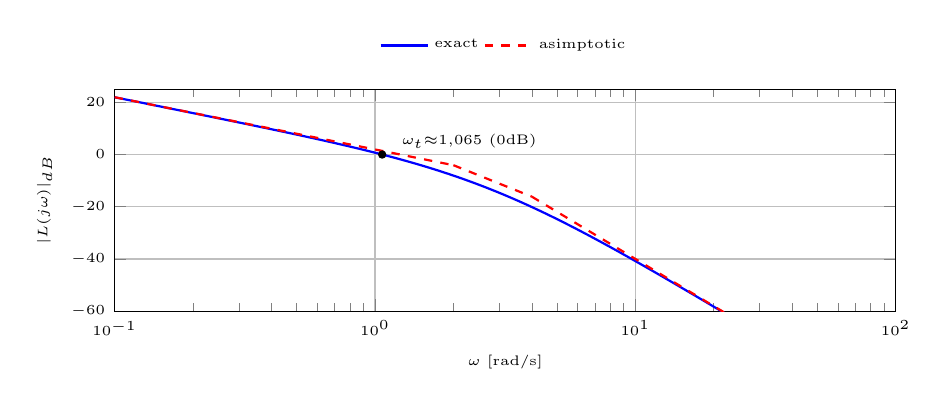
\begin{tikzpicture}
\begin{semilogxaxis}[
    width=11.5cm, height=4.4cm,
    xlabel={\tiny $\omega$ [rad/s]}, ylabel={\tiny $|L(j\omega)|_{dB}$},
    xmin=0.1, xmax=100, ymin=-60, ymax=25,
    grid=major, tick label style={font=\tiny},
    legend style={font=\tiny,at={(0.5,1.28)},anchor=north,legend columns=2,draw=none}
]
\addplot[domain=0.1:100,samples=200,blue,thick] {20-20*ln(x)/ln(10)-10*ln(x^2+4)/ln(10)-10*ln(x^2+16)/ln(10)};
\addplot[domain=0.1:2,samples=2,red,thick,dashed] {20*ln(1.25/x)/ln(10)};
\addplot[domain=2:4,samples=2,red,thick,dashed] {20*ln(0.625)/ln(10)-40*ln(x/2)/ln(10)};
\addplot[domain=4:100,samples=2,red,thick,dashed] {20*ln(0.625)/ln(10)-40*ln(2)/ln(10)-60*ln(x/4)/ln(10)};
\addplot[only marks,mark=*,mark size=1.3pt,black] coordinates {(1.065,0)};
\node[font=\tiny] at (axis cs:2.3,5) {$\omega_t{\approx}1{,}065$ (0dB)};
\legend{exact,asimptotic}
\end{semilogxaxis}
\end{tikzpicture}

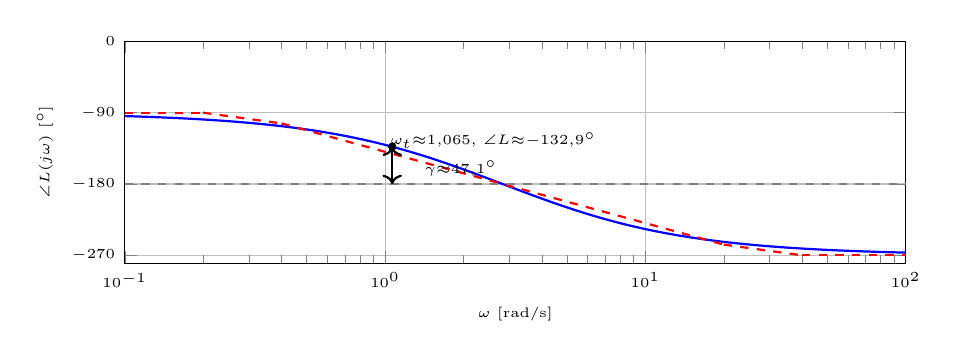
\begin{tikzpicture}
\begin{semilogxaxis}[
    width=11.5cm, height=4.4cm,
    xlabel={\tiny $\omega$ [rad/s]}, ylabel={\tiny $\angle L(j\omega)\ [^\circ]$},
    xmin=0.1, xmax=100, ymin=-280, ymax=0,
    ytick={-270,-180,-90,0}, grid=major, tick label style={font=\tiny}
]
\addplot[domain=0.1:100,samples=200,blue,thick] {-90-atan(x/2)-atan(x/4)};
\addplot[domain=0.1:0.2,samples=2,red,thick,dashed] {-90};
\addplot[domain=0.2:0.4,samples=2,red,thick,dashed] {-90-45*ln(5*x)/ln(10)};
\addplot[domain=0.4:20,samples=2,red,thick,dashed] {-90-45*ln(5*x)/ln(10)-45*ln(2.5*x)/ln(10)};
\addplot[domain=20:40,samples=2,red,thick,dashed] {-180-45*ln(2.5*x)/ln(10)};
\addplot[domain=40:100,samples=2,red,thick,dashed] {-270};
\addplot[domain=0.1:100,samples=2,gray,dashed] {-180};
\addplot[only marks,mark=*,mark size=1.3pt,black] coordinates {(1.065,-132.9)};
\draw[<->,thick] (axis cs:1.065,-180) -- (axis cs:1.065,-132.9);
\node[font=\tiny,anchor=west] at (axis cs:1.3,-160) {$\gamma{\approx}47{,}1^\circ$};
\node[font=\tiny] at (axis cs:2.6,-125) {$\omega_t{\approx}1{,}065$, $\angle L{\approx}{-}132{,}9^\circ$};
\end{semilogxaxis}
\end{tikzpicture}
\end{center}
\tip{\textit{Observație grafic:} pun degetul pe curba de modul (albastru) acolo unde taie linia de $0$dB — asta e $\omega_t{\approx}1{,}065$rad/s, calculat algebric mai sus. Cobor cu aceeași abscisă $\omega_t$ pe graficul de fază: citesc direct $\angle L(j\omega_t){\approx}{-}132{,}9^\circ$. Marginea de fază $\gamma$ e distanța (pe verticală) de la această valoare până la linia de referință $-180^\circ$ (gri, punctată) — cu cât „mai sus" e curba de fază față de $-180^\circ$ la frecvența de tăiere, cu atât sistemul e mai stabil în buclă închisă. Aici $\gamma{\approx}47{,}1^\circ{>}0\Rightarrow$ stabil, coerent cu a) ($k{=}10{<}48$).}

\textbf{Subiect 4 — locul rădăcinilor, $G(s)=\dfrac{K(s+3)}{s(s+4)(s^2+4s+6)}$ (reacție unitară):}

\textit{Rezolvare (pașii \hyperref[sec:14]{secțiunii 14}, aceeași rețetă ca la Subiectul D din \hyperref[sec:21]{secțiunea 21}):} poli: $p_1{=}0,\,p_2{=}{-}4,\,p_{3,4}{=}{-}2\pm j1{,}41$ (din $s^2{+}4s{+}6{=}0$). Zero: $z_1{=}{-}3$. $n{=}4,\,m{=}1\Rightarrow n-m=3$ asimptote (pasul 4).

Axa reală (pasul 3, regula parității impare): poli/zerouri reale, în ordine, $-4,-3,0$ (perechea complexă $-2\pm1{,}41j$ nu contează, nefiind pe axa reală). Verific numărul de poli+zerouri reale la \textbf{dreapta} fiecărui segment:
\begin{itemize}
\item $(-3,0)$: la dreapta e doar polul din $0$ $\Rightarrow$ $1$ (impar) $\Rightarrow$ pe locus;
\item $(-4,-3)$: la dreapta sunt polul $0$ și zero-ul $-3$ $\Rightarrow$ $2$ (par) $\Rightarrow$ NU e pe locus;
\item $(-\infty,-4)$: la dreapta sunt $0,-3,-4$ $\Rightarrow$ $3$ (impar) $\Rightarrow$ pe locus.
\end{itemize}
Deci $(-3,0)$ e ramură directă pol$\to$zero (pleacă din polul $0$ la $K{=}0$ și ajunge în zero-ul $-3$ la $K{\to}\infty$; $K(s)$ crește monoton pe interval, fără punct de ramificație — vezi pasul 6 mai jos), iar $(-\infty,-4)$ e ramură directă pol$\to\infty$ (pleacă din polul $-4$ și merge direct spre $-\infty$, chiar pe asimptota $180^\circ$).

Fără puncte de ramificație (pasul 6): pun $K$ ca funcție de $s$, izolând-o din ecuația caracteristică $1+K(s+3)/[s(s+4)(s^2+4s+6)]=0$:
$$K(s)=-\dfrac{s(s+4)(s^2+4s+6)}{s+3}$$
Punctele de ramificație sunt soluțiile reale ale $dK/ds=0$ (derivata unui cât). Derivând și aducând totul la același numitor, condiția $dK/ds{=}0$ revine la a anula numărătorul rezultat:
$$3s^4+28s^3+94s^2+132s+72=0$$
Acest polinom nu are nicio rădăcină reală (se verifică ușor numeric — rămâne strict pozitiv pentru orice $s$ real) $\Rightarrow$ nu există puncte de ramificație.

\tip{\textit{Ce e un „punct de rupere" (breakaway point) — și dacă e valabil la noi:} da, conceptul e complet valabil aici, e chiar pasul 6 din rețeta generală (\hyperref[sec:14]{secțiunea 14}) — „punct de rupere" și „punct de ramificație" sunt aceeași noțiune (denumiri diferite prin diverși profesori/cărți); pur și simplu, în ACEST exercițiu, nu există unul. Un punct de rupere e locul de pe axa reală unde \textbf{două ramuri ale locului se despart} de pe axa reală în planul complex (sau, invers, unde două ramuri complexe se \textbf{reîntâlnesc} pe axa reală — atunci unii îi zic specific „punct de intrare"). Fizic: pe un segment de pe axa reală care aparține locului, dacă acolo se apropie \textbf{două rădăcini reale distincte} (venind din doi poli, sau din doi zerouri, sau dintr-un pol și un zero, pe măsură ce $K$ crește), $K(s)$ crește până când cele două rădăcini „se ciocnesc" într-un punct — acolo $K(s)$ are un maxim (sau minim) local — și pentru $K$ dincolo de acel punct, cele două rădăcini devin o pereche complex conjugată, adică locul „se rupe" de pe axa reală, simetric față de ea. Matematic, un maxim/minim local al lui $K(s)$ înseamnă exact $dK/ds{=}0$ — de-aici rețeta pasul 6.}

\tip{\textit{De ce nu avem așa ceva aici:} uită-te la cele două segmente găsite la pasul 3, $(-3,0)$ și $(-\infty,-4)$. Fiecare e parcurs de o \textbf{singură} ramură (nu de două care se apropie una de alta): $(-3,0)$ e traversat de ramura care pleacă din polul $0$ și merge direct la zero-ul $-3$ (capetele segmentului SUNT deja cele două rădăcini — nu se apropie nimic în interior), iar $(-\infty,-4)$ e traversat de ramura care pleacă din polul $-4$ spre $-\infty$ (aici doar un capăt e finit). Ca să existe un candidat de punct de rupere, ai nevoie de \textbf{minim doi poli (sau două zerouri) reali, ambii capete ale ACELUIAȘI segment de pe locus}, care se apropie unul de celălalt când $K$ crește — la noi asta nu se întâmplă pe niciun segment, deci geometric nici nu era de așteptat vreun punct de rupere; calculul $dK/ds{=}0\Rightarrow3s^4{+}28s^3{+}94s^2{+}132s{+}72{=}0$ (fără rădăcini reale) doar confirmă riguros ce sugerează deja desenul axei reale. (Compară cu Subiectul D din \hyperref[sec:21]{secțiunea 21}, unde EXISTĂ două puncte de rupere valide — acolo segmentele $[-2,-1]$ și $[-4,-3]$ au fiecare doi poli reali la capete care se apropie unul de altul.)}

Asimptote (pasul 4, $\theta_k{=}\tfrac{180^\circ(2k+1)}{n-m}$, $\sigma_a{=}\tfrac{\sum p_i-\sum z_j}{n-m}$): centrul $\sigma_a{=}\dfrac{(0-4-2-2)-(-3)}3{=}-\dfrac53\approx-1{,}67$; unghiuri $60^\circ,180^\circ,300^\circ$.

Unghi de plecare din $p_3{=}{-}2{+}1{,}41j$ (pasul 5): calculez unghiul (față de axa reală pozitivă) al vectorului de la fiecare pol/zero ceilalți până la $p_3$ — practic „din ce direcție se vede $p_3$" de la fiecare. Rețetă generală (unghiul unui vector $a+jb$, cu $\mathrm{arctg}$ aplicat DOAR pe valorile absolute, apoi corectat după cadran):
\begin{keyeq}\color{red!65!black}
$$\angle(a+jb)=\begin{cases}
\mathrm{arctg}\dfrac{|b|}{|a|} & \text{cadranul I}\ (a{>}0,\,b{>}0)\\[5pt]
180^\circ-\mathrm{arctg}\dfrac{|b|}{|a|} & \text{cadranul II}\ (a{<}0,\,b{>}0)\\[5pt]
-\Big(180^\circ-\mathrm{arctg}\dfrac{|b|}{|a|}\Big) & \text{cadranul III}\ (a{<}0,\,b{<}0)\\[5pt]
-\,\mathrm{arctg}\dfrac{|b|}{|a|} & \text{cadranul IV}\ (a{>}0,\,b{<}0)
\end{cases}$$
\end{keyeq}
(cazuri speciale, fără arctg: $a{=}0\Rightarrow\pm90^\circ$ după semnul lui $b$; $b{=}0\Rightarrow0^\circ$ dacă $a{>}0$, $180^\circ$ dacă $a{<}0$.) Aceeași rețetă e folosită și mai jos, la argumentul lui $G(j4)$ din Subiectul 5.

Aplic rețeta pe cei 4 vectori de la ceilalți poli/zero până la $p_3$:
\begin{itemize}
\item de la $p_1{=}0$: vectorul $p_3{-}p_1{=}{-}2{+}1{,}41j$ (cadranul II) $\Rightarrow$ unghi $=180^\circ-\mathrm{arctg}\tfrac{1,41}2\approx144{,}7^\circ$
\item de la $p_2{=}{-}4$: vectorul $p_3{-}p_2{=}2{+}1{,}41j$ (cadranul I) $\Rightarrow$ unghi $=\mathrm{arctg}\tfrac{1,41}2\approx35{,}3^\circ$
\item de la $p_4{=}{-}2{-}1{,}41j$ (polul conjugat): vectorul $p_3{-}p_4{=}0{+}2{,}82j$ (pur imaginar, drept în sus) $\Rightarrow$ unghi $=90^\circ$
\item de la zero-ul $z_1{=}{-}3$: vectorul $p_3{-}z_1{=}1{+}1{,}41j$ (cadranul I) $\Rightarrow$ unghi $=\mathrm{arctg}\tfrac{1,41}1\approx54{,}7^\circ$
\end{itemize}
Aplic formula (pasul 5, \hyperref[sec:14]{secțiunea 14}) $\varphi_p{=}180^\circ{-}\sum\text{unghiuri poli}{+}\sum\text{unghiuri zerouri}$ — pe scurt, poli scad, zerouri adună:
\begin{keyeq}\color{red!65!black}
$$\varphi_p=180^\circ-\underbrace{(144{,}7^\circ+35{,}3^\circ+90^\circ)}_{\text{cei 3 poli}}+\underbrace{54{,}7^\circ}_{\text{zero-ul}}\approx-35{,}3^\circ\qquad\text{(simetric }+35{,}3^\circ\text{ din }p_4\text{)}$$
\end{keyeq}

Intersecția cu axa $j\omega$ (pasul 7, criteriul Routh — recapitulare rețetă generală: \hyperref[sec:14b]{secțiunea 14b}): pornesc de la ecuația caracteristică $1{+}G(s){=}0$, adică $s(s{+}4)(s^2{+}4s{+}6)+K(s{+}3)=0$.

\textit{De unde vine polinomul de gradul 4} — expandez întâi partea fără $K$: notez $u{=}s^2{+}4s$ (din $s(s{+}4)$), rămâne
$$u(u{+}6)=u^2+6u=(s^2{+}4s)^2+6(s^2{+}4s)=(s^4{+}8s^3{+}16s^2)+(6s^2{+}24s)=s^4+8s^3+22s^2+24s$$
adaug $K(s{+}3){=}Ks{+}3K$ — termenii cu $s^1$ se adună ($24s{+}Ks$), restul rămân separați:
\begin{keyeq}\color{red!65!black}
$$s^4+8s^3+22s^2+(24+K)s+3K=0$$
\end{keyeq}

Tablou Routh:
\begin{center}
\begin{tabular}{c|cc}
$s^4$ & $1$ & $22$ \quad $3K$\\
$s^3$ & $8$ & $24{+}K$ \quad $0$\\
$s^2$ & $b_1{=}\dfrac{8{\cdot}22-1{\cdot}(24{+}K)}8{=}\dfrac{152-K}8$ & $3K$\\
$s^1$ & $c_1{=}\dfrac{b_1(24{+}K)-8{\cdot}3K}{b_1}{=}\dfrac{3648-64K-K^2}{152-K}$ & \\
$s^0$ & $3K$ &
\end{tabular}
\end{center}

Limita de stabilitate (rândul $s^1$ devine tot zero) $\Rightarrow c_1{=}0$:
$$3648-64K-K^2=0\ \Rightarrow\ K^2+64K-3648=0\ \Rightarrow\ K_l=\dfrac{-64+\sqrt{64^2+4{\cdot}3648}}2\approx36{,}3$$
Odată găsit $K_l$, $s{=}\pm j\omega$ NU vin din rândul $s^1$ (care e zero), ci din rândul de deasupra ($s^2$), tratat ca \textbf{polinom auxiliar}: $b_1s^2+3K_l=0\Rightarrow s^2=-3K_l/b_1$; cu $b_1{=}(152{-}36{,}3)/8\approx14{,}46$: $s^2\approx-7{,}55\Rightarrow s\approx\pm j2{,}75$.
\begin{keyeq}\color{red!65!black}
$$K_l\approx36{,}3,\qquad s\approx\pm j2{,}75$$
\end{keyeq}

\textit{Verificare prin metoda alternativă} $s{=}j\omega$ (aceeași idee, altă tehnică — pun direct $s{=}j\omega$ în ecuația caracteristică $s^4{+}8s^3{+}22s^2{+}(24{+}K)s{+}3K{=}0$ și separ real/imaginar):
$$(\jmath\omega)^4+8(\jmath\omega)^3+22(\jmath\omega)^2+(24{+}K)(\jmath\omega)+3K=\underbrace{\big[\omega^4-22\omega^2+3K\big]}_{\text{Re}}+\underbrace{\big[{-}8\omega^3+(24{+}K)\omega\big]}_{\text{Im}}\jmath=0$$
Pun Re$=0$ și Im$=0$ (sistem de 2 ecuații, 2 necunoscute $\omega,K$):
\begin{keyeq}\color{red!65!black}
$$\text{Im}=0:\ \omega\big[{-}8\omega^2+(24{+}K)\big]=0\ \xRightarrow{\omega\ne0}\ \omega^2=\dfrac{24+K}8\qquad\qquad \text{Re}=0:\ \omega^4-22\omega^2+3K=0$$
\end{keyeq}
Înlocuiesc $\omega^2$ din prima ecuație în a doua ($\times64$ ca să scap de fracții):
$$\Big(\dfrac{24{+}K}8\Big)^2-22\cdot\dfrac{24{+}K}8+3K=0\ \xrightarrow{\times64}\ (24{+}K)^2-176(24{+}K)+192K=0$$
Expandez $(24{+}K)^2=576{+}48K{+}K^2$ și $176(24{+}K)=4224{+}176K$:
$$576{+}48K{+}K^2-4224-176K+192K=0\ \Rightarrow\ K^2+64K-3648=0$$
\textbf{Exact aceeași ecuație ca la Routh} (linia $c_1{=}0$ de mai sus) $\Rightarrow K_l\approx36{,}3$. Apoi $\omega^2=(24{+}K_l)/8=(24{+}36{,}3)/8\approx7{,}54\Rightarrow\omega\approx2{,}75$ — identic cu rezultatul din tabloul Routh, cum trebuia.
\tip{Cele două metode dau mereu același rezultat (verifică ecuația caracteristică o singură dată, doar tehnica de rezolvare diferă) — bun de folosit una ca probă pentru cealaltă dacă ai timp la examen.}

\begin{center}
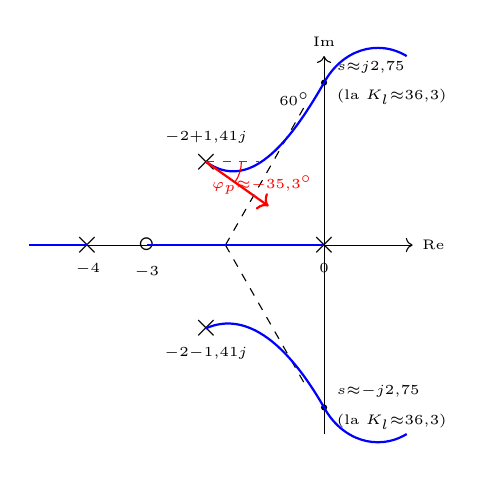
\begin{tikzpicture}[scale=0.75]
\draw[->] (-5,0) -- (1.5,0) node[right]{\tiny Re};
\draw[->] (0,-3.2) -- (0,3.2) node[above]{\tiny Im};
\node at (0,0){\large$\times$}; \node[below] at (0,-0.15){\tiny $0$};
\node at (-4,0){\large$\times$}; \node[below] at (-4,-0.15){\tiny $-4$};
\node at (-2,1.41){\large$\times$}; \node[above] at (-2,1.56){\tiny $-2{+}1{,}41j$};
\node at (-2,-1.41){\large$\times$}; \node[below] at (-2,-1.56){\tiny $-2{-}1{,}41j$};
\node at (-3,0){\large$\circ$}; \node[below] at (-3,-0.2){\tiny $-3$};
\filldraw (0,2.75) circle (1.2pt); \node[right,align=left] at (0.05,2.75){\tiny $s{\approx}j2{,}75$\\[-1pt]\tiny(la $K_l{\approx}36{,}3$)};
\filldraw (0,-2.75) circle (1.2pt); \node[right,align=left] at (0.05,-2.75){\tiny $s{\approx}{-}j2{,}75$\\[-1pt]\tiny(la $K_l{\approx}36{,}3$)};
\draw[dashed] (-1.67,0)--(-0.3,2.4); \node[above] at (-0.5,2.2){\tiny $60^\circ$};
\draw[dashed] (-1.67,0)--(-0.3,-2.4);
\draw[dashed] (-1.67,0)--(-5,0);
\draw[thick,blue] (0,0) -- (-3,0);
\draw[thick,blue] (-4,0) -- (-5,0);
\draw[thick,blue] (-2,1.41) .. controls (-1.27,0.89) and (-0.6,1.7) .. (0,2.75);
\draw[thick,blue] (0,2.75) .. controls (0.3,3.3) and (0.9,3.5) .. (1.4,3.2);
\draw[thick,blue] (-2,-1.41) .. controls (-1.3,-1.1) and (-0.6,-1.7) .. (0,-2.75);
\draw[thick,blue] (0,-2.75) .. controls (0.3,-3.3) and (0.9,-3.5) .. (1.4,-3.2);
\draw[dashed,red] (-2,1.41) -- (-1.1,1.41);
\draw[->,red,thick] (-2,1.41) -- (-0.94,0.66);
\draw[red] (-1.4,1.41) arc (0:-35.3:0.6);
\node[red] at (-1.05,1.02){\tiny $\varphi_p{\approx}{-}35{,}3^\circ$};
\end{tikzpicture}
\end{center}
\begin{center}\tiny\color{red!65!black} roșu: tangenta locusului (unghiul de plecare) exact în $p_3$ — direcția inițială a curbei la $K{=}0^+$; arcul e măsurat de la orizontală (referință, punctat) până la tangentă. Curba albastră pornește pe această tangentă, apoi se curbează spre $j2{,}75$ (unde intersectează axa $j\omega$ la $K_l$) și abia la $s\to\infty$ devine paralelă cu asimptota de $60^\circ$ (linia punctată neagră).\end{center}

\tip{\textit{De ce ramura din polii complecși NU pleacă direct pe direcția asimptotei:} unghiul de plecare $\varphi_p$ (calculat mai sus, $\approx{-}35{,}3^\circ$) și unghiul asimptotei ($60^\circ$) sunt \textbf{două lucruri diferite, valabile în două regiuni diferite ale planului} — nu ai niciun motiv să te aștepți să coincidă:
\begin{itemize}
\item $\varphi_p$ descrie direcția locusului DOAR în vecinătatea imediată a polului $p_3$, la $K{\to}0^+$ — vine din condiția de fază exactă $\angle G(s)H(s){=}180^\circ$, evaluată chiar în $s{=}p_3$, unde pozițiile EXACTE ale celorlalți 3 poli/zero contează (fiecare „trage" din direcția lui, la distanțe comparabile);
\item unghiul asimptotei descrie direcția locusului DOAR când $s\to\infty$ ($K\to\infty$) — la distanțe foarte mari față de origine, toate cele 4 puncte finite (poli+zero) par „grupate în același loc" (comparate cu distanța uriașă până la $s$), efectele lor individuale devin neglijabile și contează doar centrul de greutate $\sigma_a$ cu unghiurile $\theta_k{=}60^\circ,180^\circ,300^\circ$.
\end{itemize}
Cele două unghiuri ar coincide DOAR printr-o coincidență geometrică — aici NU coincid ($-35{,}3^\circ\ne60^\circ$), deci ramura e OBLIGATĂ să se \textbf{curbeze} continuu de la un unghi la celălalt pe măsură ce $K$ crește: pleacă tangentă la $-35{,}3^\circ$ (roșu, în desen), se curbează prin cadranul II, taie axa imaginară la $j2{,}75$ (unde $K{=}K_l{\approx}36{,}3$), și abia mult mai departe de origine direcția ei se apropie de cea a asimptotei punctate de $60^\circ$. Desenul e corect făcut — segmentul desenat (limitat de spațiul paginii) pur și simplu nu ajunge suficient de departe încât linia să pară vizual paralelă cu asimptota; comportarea REALĂ a curbei (calculată prin cele două rețete, unghi de plecare + asimptotă) e cea corectă, doar apropierea perfectă de asimptotă se întâmplă abia la $s\to\infty$, nu pe porțiunea desenabilă pe hârtie. (Aceeași idee la exemplul din \hyperref[sec:14]{secțiunea 14}, $G(s){=}K/[s(s{+}1)(s^2{+}4s{+}13)]$: unghiul de plecare din polul complex e $\approx{-}142{,}2^\circ$, complet diferit de asimptotele la $\pm45^\circ,\pm135^\circ$ — și acolo ramura se curbează la fel, de la unghiul de plecare spre cel mai apropiat unghi de asimptotă, $135^\circ$.)}

\textbf{Subiect 5 — $G(s)=\dfrac9{s^2+6s+9}$, $u(t)=5\sin4t$:}

Formula generală (\hyperref[sec:6]{secțiunea 6}), pentru $u(t)=U\sin\omega t$: $y_{st}(t)=U|G(j\omega)|\sin(\omega t+\varphi)$, cu $|G(j\omega)|,\varphi=\arg G(j\omega)$ calculate din $G(s)$ evaluat în $s{=}j\omega$.

\textit{Aplicare:} $\omega_n{=}3,\ \zeta{=}1$ (amortizare critică — cf. \hyperref[sec:12]{secțiunea 12}, la $\zeta{>}0{,}707$ oricum nu ar exista vârf de rezonanță); $\omega{=}4\ne\omega_n$, deci calculăm direct $G(j4)$ — înlocuiesc $s{=}j4$ în numitor:
$$(j4)^2+6(j4)+9=-16+24j+9=-7+24j$$
\textit{Modulul} (Pitagora, triplet $7$-$24$-$25$): $|{-}7{+}24j|=\sqrt{7^2{+}24^2}=\sqrt{625}=25\ \Rightarrow\ |G(j4)|=\dfrac9{25}=0{,}36$.

\textit{Teorie — argumentul unui cât (sau produs) de numere complexe:} scrise în formă polară $z=re^{j\theta}$ ($r{=}|z|$, $\theta{=}\angle z$):
\begin{keyeq}\color{red!65!black}
$$z_1z_2=r_1r_2\,e^{j(\theta_1+\theta_2)}\ \text{(unghiurile se ADUNĂ)}\qquad\qquad \dfrac{z_1}{z_2}=\dfrac{r_1}{r_2}\,e^{j(\theta_1-\theta_2)}\ \text{(unghiurile se SCAD)}$$
\end{keyeq}
la fel pentru module: $|z_1z_2|{=}|z_1||z_2|$, $|z_1/z_2|{=}|z_1|/|z_2|$ — de-aia calculezi modulul și unghiul \textbf{separat pentru fiecare factor}, apoi combini (regăsești aceeași idee, cu mai mulți factori, la unghiul de plecare din \hyperref[sec:15]{secțiunea 15}: $\angle G=\sum\angle(\text{zerouri})-\sum\angle(\text{poli})$).

\textbf{Unghiul unui factor $a{+}jb$, toate cazurile posibile:}
\begin{itemize}
\item real pozitiv ($a{>}0,b{=}0$): unghi $0^\circ$ — \textbf{fără arctg};
\item real negativ ($a{<}0,b{=}0$): unghi $180^\circ$ — \textbf{fără arctg};
\item imaginar pur, $b{>}0$ ($a{=}0$): unghi $90^\circ$ — \textbf{fără arctg};
\item imaginar pur, $b{<}0$ ($a{=}0$): unghi $-90^\circ$ — \textbf{fără arctg};
\item complex general ($a{\ne}0$ și $b{\ne}0$, orice cadran): rețeta pe cadrane $\angle(a{+}jb)$ din \hyperref[sec:15]{secțiunea 15} (cu $\mathrm{arctg}\tfrac{|b|}{|a|}$, corectat după cadran).
\end{itemize}

\textit{Aplicare pe $G(j4)=\dfrac9{-7+24j}$:} numărătorul $9$ e real pozitiv $\Rightarrow$ unghi $0^\circ$ (cazul special, fără arctg). Numitorul $-7{+}24j$ are partea reală negativă și partea imaginară pozitivă $\Rightarrow$ e în cadranul II (cazul general) — unghiul dintr-un cadran II se calculează ca $180^\circ$ minus unghiul de referință $\mathrm{arctg}\big(\tfrac{|\mathrm{Im}|}{|\mathrm{Re}|}\big)=\mathrm{arctg}\tfrac{24}7\approx73{,}7^\circ$, deci unghiul numitorului $\approx180^\circ-73{,}7^\circ=106{,}3^\circ$. Aplic regula împărțirii (unghiurile se scad):
$$\varphi=\angle(\text{numărător})-\angle(\text{numitor})=0^\circ-106{,}3^\circ=-106{,}3^\circ$$
Deci $U{=}5$, $|G(j4)|{=}0{,}36$:
\begin{keyeq}\color{red!65!black}
$$y_{st}(t)=5\cdot0{,}36\sin(4t-106{,}3^\circ)\approx1{,}8\sin(4t-106{,}3^\circ)$$
\end{keyeq}

\begin{center}
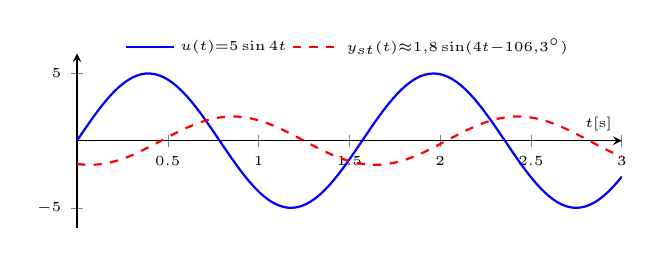
\begin{tikzpicture}
\begin{axis}[width=8.5cm,height=3.8cm,axis lines=middle,xlabel={\tiny $t$[s]},xtick={0,0.5,...,3},tick label style={font=\tiny},ytick={-5,5},yticklabels={\tiny$-5$,\tiny$5$},ymin=-6.5,ymax=6.5,xmin=0,xmax=3,
legend style={font=\tiny,at={(0.5,1.15)},anchor=north,legend columns=2,draw=none}]
\addplot[domain=0:3,samples=120,blue,thick] {5*sin(4*x*180/pi)};
\addplot[domain=0:3,samples=120,red,thick,dashed] {1.8*sin(4*x*180/pi-106.3)};
\legend{$u(t){=}5\sin4t$,$y_{st}(t){\approx}1{,}8\sin(4t{-}106{,}3^\circ)$}
\end{axis}
\end{tikzpicture}
\end{center}

\begin{keyeq}\color{red!65!black}
\textbf{Teorie (bilet oficial 2026):}
\begin{enumerate}
\item unghiul de fază al factorului de amplificare $K$: $0^\circ$ ($K{>}0$) sau $180^\circ$ ($K{<}0$) — constant, independent de $\omega$.
\item aproximarea în frecvență a caracteristicii amplitudine-pulsație pt. ordinul doi (\hyperref[sec:7]{secțiunea 7}): asimptotă $0$dB sub $\omega_n$, pantă $-40$dB/dec peste $\omega_n$, frângere chiar la $\omega{=}\omega_n$ (indiferent de $\zeta$), eventual vârf de rezonanță lângă $\omega_n$ dacă $\zeta$ e mic ($\le0{,}707$).
\item la intrare sinusoidală $u(t){=}U\sin\omega t$, ieșirea în regim staționar e tot sinusoidală, \textbf{aceeași frecvență} $\omega$, amplitudine $U|G(j\omega)|$ și defazaj $\angle G(j\omega)$ față de intrare (\hyperref[sec:6]{secțiunea 6}).
\item schema bloc de reglare pentru un sistem MIMO (2 intrări–2 ieșiri): fiecare ieșire e comparată cu propria referință (2 sumatoare/regulatoare separate), dar procesul cuplează ambele canale prin $G_{12},G_{21}$ (\hyperref[sec:13]{secțiunea 13}):
\end{enumerate}
\end{keyeq}

\begin{center}
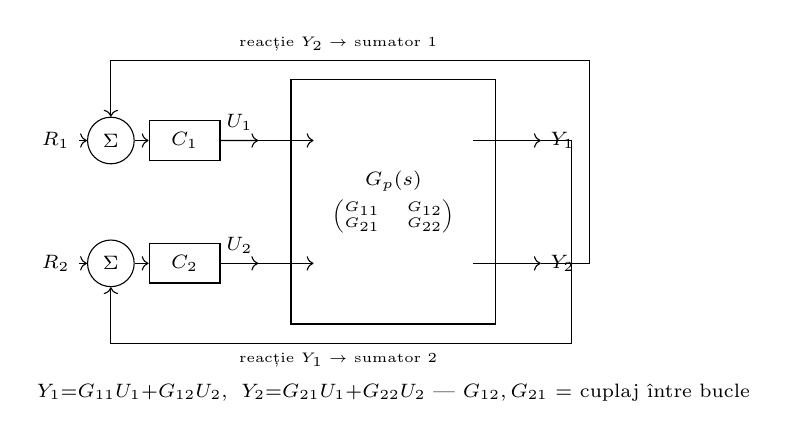
\begin{tikzpicture}[scale=0.78, every node/.style={font=\scriptsize}]
\node (r1) at (0,2) {$R_1$};
\node[draw,circle,minimum size=0.4cm] (s1) at (0.9,2) {$\Sigma$};
\draw[->] (r1)--(s1);
\node[draw,minimum width=0.9cm,minimum height=0.5cm] (c1) at (2.1,2) {$C_1$};
\draw[->] (s1)--(c1);
\draw[->] (c1) -- (3.3,2) node[above,pos=0.5]{$U_1$};

\node (r2) at (0,0) {$R_2$};
\node[draw,circle,minimum size=0.4cm] (s2) at (0.9,0) {$\Sigma$};
\draw[->] (r2)--(s2);
\node[draw,minimum width=0.9cm,minimum height=0.5cm] (c2) at (2.1,0) {$C_2$};
\draw[->] (s2)--(c2);
\draw[->] (c2) -- (3.3,0) node[above,pos=0.5]{$U_2$};

\node[draw,minimum width=2.6cm,minimum height=3.1cm,align=center] (gp) at (5.5,1) {$G_p(s)$\\[2pt]\tiny$\begin{pmatrix}G_{11}&G_{12}\\G_{21}&G_{22}\end{pmatrix}$};
\draw[->] (3.3,2) -- (4.2,2);
\draw[->] (3.3,0) -- (4.2,0);

\draw[->] (6.8,2) -- (7.9,2) node[right]{$Y_1$};
\draw[->] (6.8,0) -- (7.9,0) node[right]{$Y_2$};

\draw[->] (7.9,2) -| (8.4,-1.3) -| (s2.south);
\node[below] at (4.6,-1.3){\tiny reacție $Y_1\to$ sumator 2};

\draw[->] (7.9,0) -| (8.7,3.3) -| (s1.north);
\node[above] at (4.6,3.3){\tiny reacție $Y_2\to$ sumator 1};

\node[align=left] at (5.5,-2.1){\scriptsize $Y_1{=}G_{11}U_1{+}G_{12}U_2$, $\;Y_2{=}G_{21}U_1{+}G_{22}U_2$ — $G_{12},G_{21}$ = cuplaj între bucle};
\end{tikzpicture}
\end{center}

\section*{20. Al doilea bilet — sesiunea vară 2026 (variantă suplimentară)}\phantomsection\label{sec:20}
\textit{Aceeași structură ca biletul din \hyperref[sec:19]{secțiunea 19} (5 subiecte + 4 întrebări de teorie, 1p fiecare), cu alte funcții de transfer — util ca al doilea exercițiu complet cu aceleași rețete, plus câteva cazuri noi (tip 0 la Bode, marginea de amplitudine calculată explicit, loc al rădăcinilor fără $K_l$).}

\textbf{Subiect 1 — $G_0(s)=\dfrac{3s+2}{s^2+6s+25}$:}

\textit{a) Model SS} (formă canonică controlabilă, \hyperref[sec:4]{secțiunea 4a}): din numitor $a_1{=}6,a_0{=}25$; din numărător $b_1{=}3,b_0{=}2$:
\begin{keyeq}\color{red!65!black}
$$A=\begin{pmatrix}0&1\\-25&-6\end{pmatrix},\ B=\begin{pmatrix}0\\1\end{pmatrix},\ C=\begin{pmatrix}2&3\end{pmatrix},\ D=0$$
\end{keyeq}

\textit{c) Răspunsul la treaptă unitară} (fracții simple, \hyperref[sec:3b]{secțiunea 3b}): poli $s^2{+}6s{+}25{=}0\Rightarrow s{=}{-}3{\pm}4j$ (complecși). $Y(s){=}G_0(s)/s{=}\dfrac As+\dfrac{Bs+C}{s^2+6s+25}$; din $s^0$: $A{=}2/25{=}0{,}08$; din $s^2$: $B{=}{-}A{=}{-}0{,}08$; din $s^1$: $C{=}3{-}6A{=}2{,}52$. Aduc numitorul la $(s{+}3)^2{+}16$ și numărătorul la $-0{,}08(s{+}3){+}2{,}76$:
\begin{keyeq}\color{red!65!black}
$$y(t)=0{,}08-0{,}08\,e^{-3t}\cos4t+0{,}69\,e^{-3t}\sin4t,\quad t\ge0\qquad(y(\infty){=}0{,}08{=}G_0(0)\ \checkmark)$$
\end{keyeq}

\textit{d) Controlabilitate:} formă canonică controlabilă $\Rightarrow$ întotdeauna controlabil (\hyperref[sec:5]{secțiunea 5}).

\textit{b) Schema bloc} (metodă generală: \hyperref[sec:4b]{secțiunea 4b}; caz canonic controlabil — 2 integratoare în cascadă, aceeași topologie ca la \hyperref[sec:19]{secțiunea 19}, doar cu alți coeficienți: $a_0{=}25,\,a_1{=}6$ pe reacție, $b_0{=}2,\,b_1{=}3$ pe ieșire):
\begin{center}
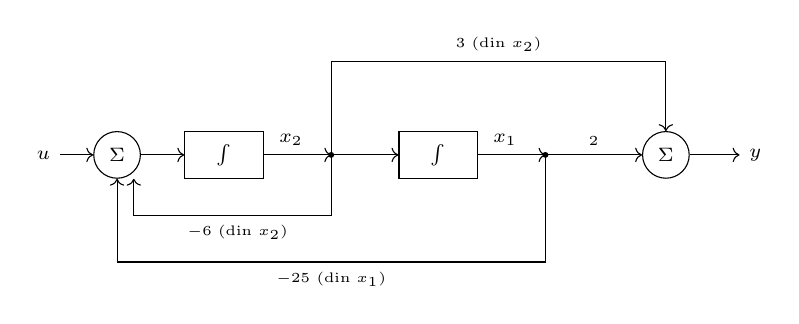
\begin{tikzpicture}[scale=0.85, every node/.style={font=\scriptsize}]
\node (u) at (0,0) {$u$};
\node[draw,circle,minimum size=0.5cm] (s1) at (1.1,0) {$\Sigma$};
\draw[->] (u)--(s1);
\node[draw,minimum width=1cm,minimum height=0.6cm] (i1) at (2.7,0) {$\int$};
\draw[->] (s1)--(i1);
\coordinate (a) at (4.3,0);
\draw[->] (i1) -- (a) node[above,pos=0.4]{$x_2$};
\filldraw (a) circle (1pt);
\node[draw,minimum width=1cm,minimum height=0.6cm] (i2) at (5.9,0) {$\int$};
\draw[->] (a) -- (i2);
\coordinate (b) at (7.5,0);
\draw[->] (i2) -- (b) node[above,pos=0.4]{$x_1$};
\filldraw (b) circle (1pt);
\node[draw,circle,minimum size=0.5cm] (sy) at (9.3,0) {$\Sigma$};
\draw[->] (b) -- (sy) node[midway,above]{\tiny $2$};
\draw[->] (a) -- ++(0,1.4) -| (sy.north);
\node[above] at (6.8,1.4){\tiny $3$ (din $x_2$)};
\draw[->] (sy) -- (10.4,0) node[right]{$y$};
\draw[->] (b) -- ++(0,-1.6) -| (s1.south);
\node[below] at (4.3,-1.6){\tiny $-25$ (din $x_1$)};
\draw[->] (a) -- ++(0,-0.9) -| ($(s1.south)+(0.25,0)$);
\node[below] at (2.9,-0.9){\tiny $-6$ (din $x_2$)};
\end{tikzpicture}
\tip{\textit{Notă:} ca și la \hyperref[sec:19]{secțiunea 19}, nu există un al doilea sumator între cele două integratoare — toate reacțiile ($-25x_1$, $-6x_2$) intră o singură dată, la primul sumator; ieșirea adună direct $2x_1{+}3x_2$ (coeficienții din $C$).}
\end{center}

\textbf{Subiect 2 — Bode pentru $G(s)=\dfrac{20(s+1)}{s+2}$ (reacție unitară, sistem TIP 0 — fără integrator!):}

\textit{Forma standard} (\hyperref[sec:7]{secțiunea 7}): $G(j\omega)=\dfrac{20(1+j\omega)}{2+j\omega}=10\dfrac{1+j\omega}{1+j\omega/2}$ (scot factorul $2$ de la numitor) $\Rightarrow K{=}10$ (NU $20$!), zero la $\omega_{f1}{=}1$, pol la $\omega_{f2}{=}2$.

\textit{Diferența cheie față de Subiectul 2 din \hyperref[sec:19]{secțiunea 19}:} acolo sistemul era tip $1$ (integrator, panta $-20$dB/dec la $\omega$ mic, fază pornind din $-90^\circ$). Aici, FĂRĂ integrator, asimptota de joasă frecvență e ORIZONTALĂ la $K_{dB}{=}20\lg10{=}20$dB, iar faza pornește din $0^\circ$. Cum zero-ul ($\omega_{f1}{=}1$) vine ÎNAINTE de pol ($\omega_{f2}{=}2$), sistemul are fază POZITIVĂ pe tot graficul (avans de fază) — opusul cazurilor de „întârziere" din restul documentului:
\begin{keyeq}\color{red!65!black}
$$|G(j\omega)|_{dB}=20\lg10+20\lg\sqrt{1+\omega^2}-20\lg\sqrt{1+(\omega/2)^2},\qquad \varphi(\omega)=\mathrm{arctg}\,\omega-\mathrm{arctg}\dfrac\omega2$$
\end{keyeq}
Asimptotic: $20$dB sub $\omega{=}1$; pantă $+20$dB/dec între $\omega{=}1$ și $\omega{=}2$ (ajunge la ${\approx}26$dB); orizontal la ${\approx}26$dB peste $\omega{=}2$ (pantele $+20$ și $-20$ se anulează).

\begin{center}
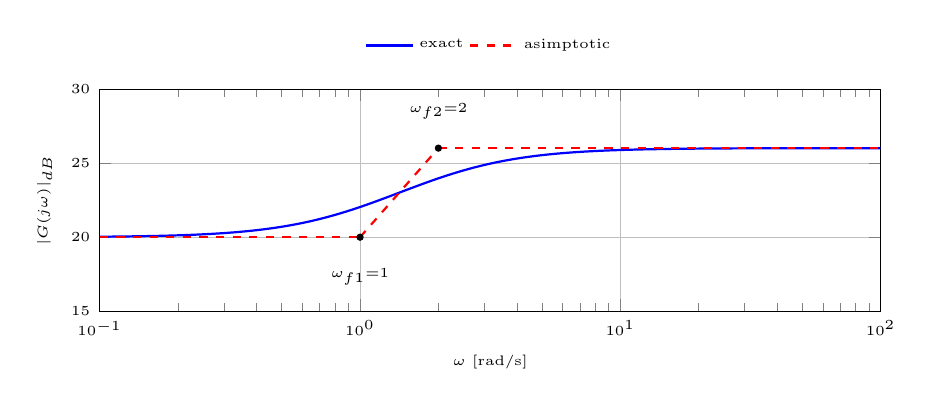
\begin{tikzpicture}
\begin{semilogxaxis}[
    width=11.5cm, height=4.4cm,
    xlabel={\tiny $\omega$ [rad/s]}, ylabel={\tiny $|G(j\omega)|_{dB}$},
    xmin=0.1, xmax=100, ymin=15, ymax=30,
    grid=major, tick label style={font=\tiny},
    legend style={font=\tiny,at={(0.5,1.28)},anchor=north,legend columns=2,draw=none}
]
\addplot[domain=0.1:100,samples=200,blue,thick] {20+10*ln(1+x^2)/ln(10)-10*ln(1+(x/2)^2)/ln(10)};
\addplot[domain=0.1:1,samples=2,red,thick,dashed] {20};
\addplot[domain=1:2,samples=2,red,thick,dashed] {20+20*ln(x)/ln(10)};
\addplot[domain=2:100,samples=2,red,thick,dashed] {20+20*ln(2)/ln(10)};
\addplot[only marks,mark=*,mark size=1.1pt,black] coordinates {(1,20)(2,26.02)};
\node[font=\tiny] at (axis cs:1,17.3) {$\omega_{f1}{=}1$};
\node[font=\tiny] at (axis cs:2,28.5) {$\omega_{f2}{=}2$};
\legend{exact,asimptotic}
\end{semilogxaxis}
\end{tikzpicture}

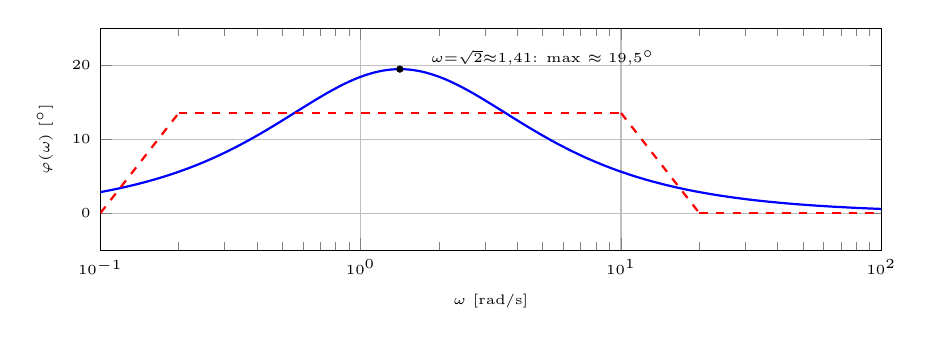
\begin{tikzpicture}
\begin{semilogxaxis}[
    width=11.5cm, height=4.4cm,
    xlabel={\tiny $\omega$ [rad/s]}, ylabel={\tiny $\varphi(\omega)\ [^\circ]$},
    xmin=0.1, xmax=100, ymin=-5, ymax=25,
    ytick={0,10,20}, grid=major, tick label style={font=\tiny}
]
\addplot[domain=0.1:100,samples=200,blue,thick] {atan(x)-atan(x/2)};
\addplot[domain=0.1:0.2,samples=2,red,thick,dashed] {45*ln(10*x)/ln(10)};
\addplot[domain=0.2:10,samples=2,red,thick,dashed] {45*ln(2)/ln(10)};
\addplot[domain=10:20,samples=2,red,thick,dashed] {90-45*ln(5*x)/ln(10)};
\addplot[domain=20:100,samples=2,red,thick,dashed] {0};
\addplot[only marks,mark=*,mark size=1.1pt,black] coordinates {(1.414,19.47)};
\node[font=\tiny] at (axis cs:5,21) {$\omega{=}\sqrt2{\approx}1{,}41$: max $\approx19{,}5^\circ$};
\end{semilogxaxis}
\end{tikzpicture}
\end{center}
\tip{\textit{Observație grafic:} curba de modul (albastru) pornește de la asimptota orizontală $20$dB (fără integrator, deci NU pleacă din $-\infty$ ca-n cazurile tip $\ge1$), urcă ușor prin zona $\omega{\in}(1,2)$ și se aplatizează iar la ${\approx}26$dB. Faza rămâne tot timpul \textbf{pozitivă} (avans, nu întârziere) — vine din faptul că zero-ul ($\omega_{f1}{=}1$) e mai aproape de origine decât polul ($\omega_{f2}{=}2$); vârful ei real ($\approx19{,}5^\circ$ la $\omega{=}\sqrt2$, media geometrică a celor două frecvențe de frângere) e puțin peste platoul asimptotic ($\approx45\lg2\approx13{,}6^\circ$), fiindcă cele două frecvențe de frângere sunt apropiate (o singură octavă distanță) și curbele exacte ale zero-ului și polului nu apucă să se „despartă" complet.}

\textit{b) Eroare staționară} — TIP $0$ (spre deosebire de toate exemplele Bode anterioare din document, care erau tip $1$) $\Rightarrow$ se folosește $K_p$, NU $K_v$ (\hyperref[sec:18]{secțiunea 18}): $K_p{=}G(0){=}20{\cdot}1/2{=}10$:
\begin{keyeq}\color{red!65!black}
$$e_{ss}(\text{treaptă})=\dfrac1{1+K_p}=\dfrac1{11}\approx0{,}091\qquad(\text{nu e zero, spre deosebire de tip}\ge1)$$
\end{keyeq}

\textbf{Subiect 3 — $G(s)=\dfrac k{s(s+2)}$, $H(s)=\dfrac1{s+3}$ (aceeași rețetă ca Subiectul 3 din \hyperref[sec:19]{secțiunea 19}, alt pol la $H(s)$, altă mărime cerută la b):}

\textit{a)} $L(s){=}\dfrac k{s(s+2)(s+3)}$; raționalizez la fel ca în \hyperref[sec:19]{secțiunea 19}: numitorul $j\omega(j\omega{+}2)(j\omega{+}3){=}{-}5\omega^2{+}j(6\omega{-}\omega^3)$, deci
\begin{keyeq}\color{red!65!black}
$$\mathrm{Re}\{L(j\omega)\}=\dfrac{-5k}{25\omega^2+(6-\omega^2)^2},\qquad \mathrm{Im}\{L(j\omega)\}=\dfrac{-k(6-\omega^2)}{\omega\big[25\omega^2+(6-\omega^2)^2\big]}$$
\end{keyeq}
Curba taie axa reală (Im$=0$) la $\omega{=}\sqrt6{\approx}2{,}449$, în punctul $-k/30$:
\begin{keyeq}\color{red!65!black}
$$0<k<30\qquad(\text{verificat prin Routh pe } s^3+5s^2+6s+k=0)$$
\end{keyeq}

\textit{Curba polară} (pentru $k{=}10$ ca reper — pentru alt $k$, scalezi toate coordonatele cu $k/10$), desenată direct din formulele Re/Im de mai sus:
\begin{center}
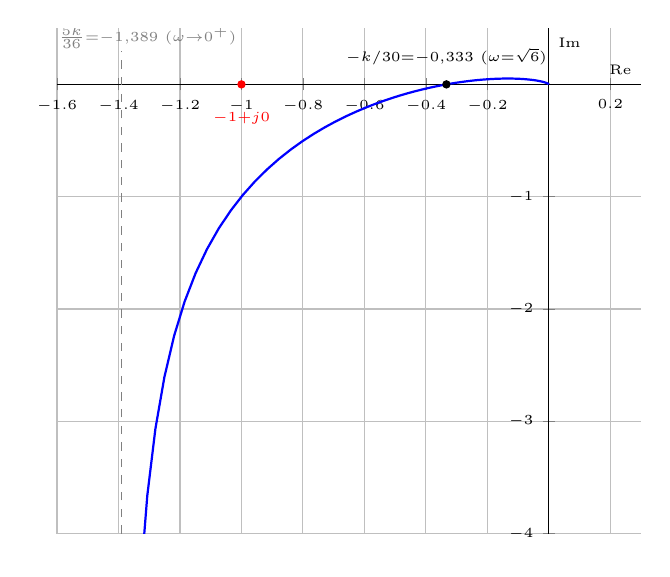
\begin{tikzpicture}
\begin{axis}[
    width=9cm, height=8cm,
    xlabel={\tiny Re}, ylabel={\tiny Im},
    xmin=-1.6, xmax=0.3, ymin=-4, ymax=0.5,
    axis lines=middle, grid=major, tick label style={font=\tiny},
    axis line style={-},
]
\addplot[domain=0.35:20, samples=300, blue, thick] ({-50/(25*x^2+(6-x^2)^2)}, {-10*(6-x^2)/(x*(25*x^2+(6-x^2)^2))});
\addplot[dashed, gray] coordinates {(-1.3889,-4)(-1.3889,0.3)};
\node[gray,font=\tiny] at (axis cs:-1.3889,0.42) {$\mathrm{Re}{=}{-}\tfrac{5k}{36}{=}{-}1{,}389$ ($\omega{\to}0^+$)};
\addplot[only marks,mark=*,mark size=1.3pt,black] coordinates {(-0.3333,0)};
\node[font=\tiny] at (axis cs:-0.3333,0.25) {$-k/30{=}{-}0{,}333$ ($\omega{=}\sqrt6$)};
\addplot[only marks,mark=*,mark size=1.3pt,red] coordinates {(-1,0)};
\node[red,font=\tiny] at (axis cs:-1,-0.3) {$-1{+}j0$};
\end{axis}
\end{tikzpicture}
\end{center}
\tip{\textit{Observație grafic:} curba pleacă (pentru $\omega\to0^+$) de pe asimptota verticală $\mathrm{Re}{=}{-}5k/36$, coboară spre $-\infty$, urcă prin cadranul III, taie axa reală o singură dată la $-k/30$ (chiar la dreapta lui $-1$, pentru $k{=}10{<}30$), trece în cadranul II și se apropie de origine tangent la semiaxa Im pozitivă. Cât timp punctul de tăiere $-k/30$ rămâne la \textbf{dreapta} lui $-1$ (adică $k{<}30$), curba nu încercuiește punctul critic $\Rightarrow$ stabil — exact concluzia de la a).}

\textit{b) Marginea de AMPLITUDINE} (nu de fază — altă mărime decât la \hyperref[sec:19]{secțiunea 19}!): $m_a{=}1/|L(j\omega_\pi)|$, cu $\omega_\pi{=}\sqrt6$ punctul de la a) unde faza e $-180^\circ$ (\hyperref[sec:11]{secțiunea 11}). Din a), $|L(j\omega_\pi)|{=}k/30$:
\begin{keyeq}\color{red!65!black}
$$m_a=\dfrac{30}k\qquad(m_{a,dB}=20\lg\dfrac{30}k)$$
\end{keyeq}
\tip{\textit{Control:} $m_a{>}1\iff k{<}30$ — exact condiția de stabilitate de la a), coerent (formulă generală valabilă pt. orice $k$ din enunțul tău, fără să alegi un exemplu numeric).}

\textbf{Subiect 4 — locul rădăcinilor, $G(s)=\dfrac{k(s+2)}{s(s^2+6s+13)}$:}

Poli: $p_1{=}0$, $p_{2,3}{=}{-}3{\pm}2j$ (din $s^2{+}6s{+}13{=}0$). Zero: $z_1{=}{-}2$. $n{=}3,m{=}1\Rightarrow2$ asimptote, unghiuri $\pm90^\circ$ (verticale la $\mathrm{Re}{=}\sigma_a$); $\sigma_a{=}\dfrac{(0{-}3{-}3)-({-}2)}2{=}{-}2$.

Axa reală (regula parității impare): segmentul $(-2,0)$ (un singur element real la dreapta — polul din origine).

Unghi de plecare din $p_2{=}{-}3{+}2j$ (unghiuri văzute de la $p_1{=}0$: $146{,}3^\circ$; de la $p_3{=}{-}3{-}2j$: $90^\circ$; de la $z_1{=}{-}2$: $116{,}6^\circ$):
\begin{keyeq}\color{red!65!black}
$$\varphi_p=180^\circ-(146{,}3^\circ+90^\circ)+116{,}6^\circ\approx60{,}3^\circ\qquad(\text{simetric}\ {-}60{,}3^\circ\ \text{din}\ p_3)$$
\end{keyeq}

Puncte de ramificație: $K(s){=}{-}s(s^2{+}6s{+}13)/(s{+}2)$, $dK/ds{=}0\Rightarrow s^3{+}6s^2{+}12s{+}13{=}0$ — singura rădăcină reală, $s{\approx}{-}3{,}71$, cade ÎN AFARA segmentului $(-2,0)$ găsit mai sus $\Rightarrow$ nu e punct de ramificație valid; locul merge direct de la polul din $0$ la zero-ul din $-2$, fără ramificație.

Intersecția cu axa $j\omega$: $s^3{+}6s^2{+}(13{+}k)s{+}2k{=}0$; rândul $s^1$ din Routh e $(78{+}4k)/6$, \textbf{mereu pozitiv} pentru orice $k{>}0$:
\begin{keyeq}\color{red!65!black}
$$\text{sistemul e stabil pentru ORICE }k>0\text{ — nu există }K_l\text{ finit (nu taie niciodată axa }j\omega\text{)}$$
\end{keyeq}
\tip{\textit{Observație:} spre deosebire de toate exemplele de loc al rădăcinilor de până acum (care găseau un $K_l$ finit), aici cele două ramuri complexe se curbează spre asimptotele verticale ($\mathrm{Re}{=}{-}2$) fără să treacă vreodată în semiplanul drept — stabilitate necondiționată în $K$.}

\textbf{Subiect 5 — $G(s)=\dfrac9{s^2+4s+9}$, $u(t)=6\sin5t$:}

$\omega_n{=}3$, $2\zeta\omega_n{=}4\Rightarrow\zeta{=}2/3{\approx}0{,}667$; $\omega{=}5\ne\omega_n$ (nu e rezonanță). La $s{=}j5$: $(j5)^2{+}4(j5){+}9{=}{-}16{+}20j$. Modulul (Pitagora): $\sqrt{16^2{+}20^2}{=}\sqrt{656}{=}4\sqrt{41}{\approx}25{,}61\Rightarrow|G(j5)|{\approx}0{,}351$. Argumentul (numitor în cadranul II, numărător real pozitiv): $\varphi{=}{-}(180^\circ{-}\mathrm{arctg}\tfrac{20}{16}){\approx}{-}128{,}7^\circ$:
\begin{keyeq}\color{red!65!black}
$$y_{st}(t)=6\cdot0{,}351\sin(5t-128{,}7^\circ)\approx2{,}11\sin(5t-128{,}7^\circ)$$
\end{keyeq}

\begin{keyeq}\color{red!65!black}
\textbf{Teorie (al doilea bilet, vară 2026):}
\begin{enumerate}
\item element de ordinul întâi pur ($1/(1{+}j\omega T)$ sau $(1{+}j\omega T)$): asimptotă orizontală ($0$dB) sub $\omega_f{=}1/T$, pantă $\mp20$dB/dec peste $\omega_f$ (semn după cum e la numărător sau numitor) — \hyperref[sec:7]{secțiunea 7}.
\item la ordinul întâi, $|G(j\omega)|$ e monoton descrescătoare $\Rightarrow M_r{=}1$, \textbf{nu există} vârf de rezonanță — \hyperref[sec:12]{secțiunea 12}.
\item indicatorii de calitate din domeniul frecvenței ai sistemului închis: vârful de rezonanță $M_r$ și lărgimea de bandă $\omega_b$ — \hyperref[sec:12]{secțiunea 12}.
\item schema bloc de reglare pt. un sistem MIMO (2 intrări–2 ieșiri): identică celei din \hyperref[sec:19]{secțiunea 19} (Teorie, pct. 4) — desenul complet e la finalul acelei secțiuni.
\end{enumerate}
\end{keyeq}

\section*{21. Bilet rezolvat complet — reluare toamnă 2025}\phantomsection\label{sec:21}
\textit{Bilet complet (5 subiecte + teorie), rezolvat integral mai jos.}

\textbf{Subiect A — model SS pentru circuit RLC serie cu variabile de stare neuzuale:} circuit $R,C,L$ serie, intrare $u(t){=}u_i(t)$ (sursă de tensiune), ieșire $y(t){=}i(t)$ (curentul din buclă). Se adoptă $x_1{=}u_R(t)$, $x_2{=}u_C(t)$ (nu $i_L,u_C$ ca de obicei!).

\textit{Rezolvare} (model general $\dot x=Ax+Bu,\ y=Cx+Du$ — \hyperref[sec:1]{secțiunea 1}; aici NU e formă canonică, fiindcă alegerea $x_1{=}u_R,x_2{=}u_C$ e impusă de enunț, nu standard): $i(t)=u_R/R=x_1/R$. Din KVL: $u_i=u_R+u_C+u_L=x_1+x_2+L\,di/dt\Rightarrow di/dt=(u_i-x_1-x_2)/L$. Cum $\dot x_1=R\,di/dt$ și $\dot x_2=du_C/dt=i/C=x_1/(RC)$:
$$\dot x_1=-\dfrac{R}{L}x_1-\dfrac{R}{L}x_2+\dfrac{R}{L}u,\qquad \dot x_2=\dfrac{1}{RC}x_1,\qquad y=\dfrac{1}{R}x_1$$
\begin{keyeq}\color{red!65!black}
$$A=\begin{pmatrix}-R/L&-R/L\\1/(RC)&0\end{pmatrix},\ B=\begin{pmatrix}R/L\\0\end{pmatrix},\ C=\begin{pmatrix}1/R&0\end{pmatrix},\ D=0$$
\end{keyeq}
\textbf{Observabilitate din schema bloc} (graf de fluență, \hyperref[sec:5]{secțiunea 5}): deși $y$ depinde direct doar de $x_1$, există cale $x_2\to\dot x_1\to x_1\to y$ (prin termenul $-\tfrac{R}{L}x_2$ din $\dot x_1$) $\Rightarrow$ \textbf{observabil}. Verificare cu $Q$: $C=(1/R,0)$, $CA=(-1/L,-1/L)$, $\det Q=-1/(RL)\ne0$ ($\checkmark$).

\textbf{Subiect B — Bode + eroare staționară pentru $G(s)=5\dfrac{0{,}1s+1}{s}$ (reacție unitară):} rezolvare pas cu pas, cu formula generală înainte de fiecare aplicare numerică (identic ca enunț cu Subiectul 2 din \hyperref[sec:19]{secțiunea 19}, biletul oficial vară 2026 — reluat aici integral, ca să ai fiecare bilet complet și autonom).

\textbf{Pasul 1 — forma generală:} orice sistem cu un integrator și un singur zero de ordinul 1 se scrie $G(j\omega)=\dfrac{K(1+j\omega T)}{j\omega}$, produs a trei factori de bază (\hyperref[sec:7]{secțiunea 7}): $K$ (câștig), $1/(j\omega)$ (integrator), $(1+j\omega T)$ (zero).

\textit{Aplicare:} $G(j\omega)=5\dfrac{1+0{,}1j\omega}{j\omega}\Rightarrow K{=}5,\ T{=}0{,}1$.

\textbf{Pasul 2 — frecvența de frângere:} formula generală $\omega_f=1/T$. \textit{Aplicare:} $\omega_f=1/0{,}1=10$rad/s — singura din tot sistemul ($K$ și integratorul nu au una).

\textbf{Pasul 3 — formula exactă} (aceeași care dă curba „exact" din grafic), din $G(j\omega)=\dfrac{K(1+j\omega T)}{j\omega}$:
\begin{keyeq}\color{red!65!black}
$$|G(j\omega)|_{dB}=20\lg K+20\lg\sqrt{1+(\omega T)^2}-20\lg\omega,\qquad \varphi(\omega)=-90^\circ+\mathrm{arctg}(\omega T)$$
\end{keyeq}
\textit{Aplicare} ($K{=}5,T{=}0{,}1$): $|G(j\omega)|_{dB}=20\lg5+20\lg\sqrt{1+(0{,}1\omega)^2}-20\lg\omega$,\quad $\varphi(\omega)=-90^\circ+\mathrm{arctg}(0{,}1\omega)$.

\textbf{Pasul 4 — regulile asimptotice generale pentru fiecare factor} (\hyperref[sec:7]{secțiunea 7}), aplicate imediat pentru $K{=}5,\,\omega_f{=}10$:
\begin{center}
\footnotesize
\begin{tabular}{|p{2.5cm}|p{6.6cm}|p{6.9cm}|}
\hline
\textbf{Factor} & \textbf{Modul (formulă generală $\to$ aplicat)} & \textbf{Fază (formulă generală $\to$ aplicat)} \\\hline
$K$ & orizontală, $K_{dB}{=}20\lg|K|$ $\to$ $20\lg5\approx14$dB & $0^\circ$ dacă $K{>}0$, $180^\circ$ dacă $K{<}0$ $\to$ $0^\circ$ \\\hline
$1/(j\omega)$ & pantă $-20$dB/dec, prin $0$dB la $\omega{=}1$ (nu depinde de $K$) & $-90^\circ$ constant $\to$ $-90^\circ$ \\\hline
$(1{+}j\omega T)$ & $0$dB sub $\omega_f{=}1/T$; pantă $+20$dB/dec peste $\to$ sub $10$: $0$dB; peste $10$: $+20$dB/dec & $0^\circ$ sub $\omega_f/10$; $+90^\circ$ peste $10\omega_f$; $+45^\circ$ la $\omega_f$ $\to$ $0^\circ$ la $1$; $+90^\circ$ la $100$; $+45^\circ$ la $10$ \\\hline
\end{tabular}
\end{center}

\textbf{Pasul 5 — le însumez} (regula de aur: dB-ii se adună, gradele se adună):

\textit{Modul:} sub $\omega_f$, formula generală a dreptei compuse $K$+integrator e $20\lg K-20\lg\omega$, care taie $0$dB la $\omega_0=K$ (rezolvi $20\lg K=20\lg\omega_0$). \textit{Aplicare:} $\omega_0{=}5$. Peste $\omega_f$, panta compusă devine $-20{+}20{=}0$dB/dec (orizontală), la nivelul general $20\lg(K/\omega_f)$. \textit{Aplicare:} $20\lg(5/10){=}20\lg0{,}5\approx-6$dB.

\textit{Fază:} formula generală asimptotică (3 drepte) e $-90^\circ$ sub $\omega_f/10$, apoi crește liniar cu $+45^\circ$/decadă până la $10\omega_f$, unde ajunge la $0^\circ$. \textit{Aplicare:} $-90^\circ$ sub $\omega{=}1$; la $\omega{=}10$ (chiar $\omega_f$) $-90{+}45{=}-45^\circ$; la $\omega{=}100$ atinge $0^\circ$.

\textbf{Pasul 6 — desenez efectiv, cu rigla, pe foaie} (algoritmul \hyperref[sec:8]{secțiunii 8}):

\textit{Pregătesc axele.} N-ai hârtie logaritmică la examen, deci axa orizontală ($\omega$) o construiești manual: marchezi puncte \textbf{egal distanțate} pentru fiecare \textbf{putere a lui 10}: $0{,}1-1-10-100-1000$. Distanța dintre oricare doi vecini e \textbf{aceeași} pe hârtie (asta e toată ideea scării log — fiecare pas la dreapta înmulțește $\omega$ cu $10$, nu adaugă un număr fix). Axa verticală: dB pentru modul, grade pentru fază.

\textit{Modul — rețetă mecanică:}
\begin{enumerate}
\item Pui un punct la $\omega{=}1$, înălțime $K_{dB}{=}14$dB (calculat la Pasul 4).
\item Din acel punct, tragi o linie dreaptă cu panta $-20$dB/decadă: mecanic, \textbf{la fiecare diviziune spre dreapta cobori cu 20}, la fiecare diviziune spre stânga urci cu 20. Deci la $\omega{=}0{,}1$ ești la $14{+}20{=}34$dB; continuând spre dreapta, la $\omega{=}10$ ai fi la $14{-}20{=}{-}6$dB.
\item \textbf{Te oprești din tras linia asta exact la $\omega_f{=}10$} — acolo intervine zero-ul (Pasul 2). De la $\omega{=}10$ încolo, schimbi panta la $0$dB/decadă (linie \textbf{orizontală}), pornind chiar de la valoarea unde ai ajuns, $-6$dB.
\item Asta e toată asimptota: coboară în linie dreaptă până la $\omega{=}10$, apoi devine plată la $-6$dB.
\item (Pentru curba exactă, albastră: rotunjești ușor colțul de la $\omega_f$, trecând cu $\approx3$dB sub asimptotă acolo — o singură frecvență de frângere de ordin 1 dă eroarea maximă de $3$dB exact în colț, vezi \hyperref[sec:7]{secțiunea 7}.)
\end{enumerate}

\textit{Fază — rețetă mecanică:}
\begin{enumerate}
\item Marchezi $\omega_f/10{=}1$ și $10\omega_f{=}100$ pe aceeași axă orizontală (le ai deja ca diviziuni).
\item Sub $\omega{=}1$: linie orizontală la $-90^\circ$.
\item Între $\omega{=}1$ și $\omega{=}100$ (exact $2$ decade): tragi o linie dreaptă de la punctul $({-}90^\circ$ la $\omega{=}1)$ până la punctul $(0^\circ$ la $\omega{=}100)$ — o urcare de $90^\circ$ pe $2$ decade, adică pantă $45^\circ$/decadă.
\item Peste $\omega{=}100$: linie orizontală la $0^\circ$.
\item \tip{\textbf{Control:} la $\omega_f{=}10$ (mijlocul segmentului înclinat, o decadă din fiecare parte) trebuie să treci exact prin $-45^\circ$ — dacă nu, ai greșit panta.}
\end{enumerate}

Rezultatul (curbe exacte cu albastru, asimptote cu roșu) e graficul de mai jos.

\textbf{Pasul 7 — eroare staționară} (formule generale $K_p,K_v$ — \hyperref[sec:18]{secțiunea 18}; tip $1$, un singur integrator): $K_p{=}\lim_{s\to0}G(s){=}\infty$, $K_v{=}\lim_{s\to0}sG(s){=}5$:
\begin{keyeq}\color{red!65!black}
$$e_{ss}(\text{treaptă})=0,\qquad e_{ss}(\text{rampă})=1/K_v=0{,}2$$
\end{keyeq}

\begin{center}
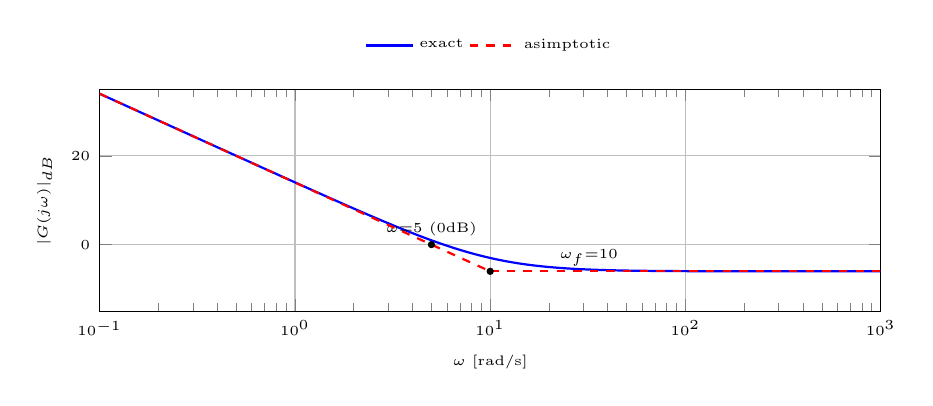
\begin{tikzpicture}
\begin{semilogxaxis}[
    width=11.5cm, height=4.4cm,
    xlabel={\tiny $\omega$ [rad/s]}, ylabel={\tiny $|G(j\omega)|_{dB}$},
    xmin=0.1, xmax=1000, ymin=-15, ymax=35,
    grid=major, tick label style={font=\tiny},
    legend style={font=\tiny,at={(0.5,1.28)},anchor=north,legend columns=2,draw=none}
]
\addplot[domain=0.1:1000,samples=200,blue,thick] {20*ln(5*sqrt(1+(0.1*x)^2)/x)/ln(10)};
\addplot[domain=0.1:10,samples=2,red,thick,dashed] {20*ln(5/x)/ln(10)};
\addplot[domain=10:1000,samples=2,red,thick,dashed] {20*ln(0.5)/ln(10)};
\addplot[only marks,mark=*,mark size=1.1pt,black] coordinates {(5,0)(10,-6.02)};
\node[font=\tiny] at (axis cs:5,3.5) {$\omega{=}5$ (0dB)};
\node[font=\tiny] at (axis cs:32,-3) {$\omega_f{=}10$};
\legend{exact,asimptotic}
\end{semilogxaxis}
\end{tikzpicture}

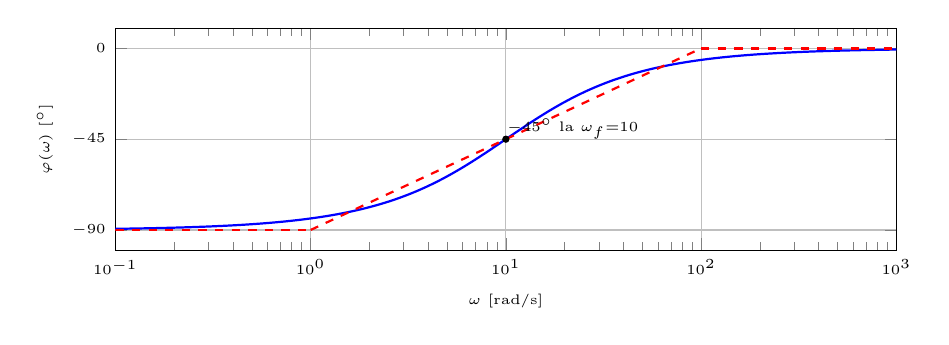
\begin{tikzpicture}
\begin{semilogxaxis}[
    width=11.5cm, height=4.4cm,
    xlabel={\tiny $\omega$ [rad/s]}, ylabel={\tiny $\varphi(\omega)\ [^\circ]$},
    xmin=0.1, xmax=1000, ymin=-100, ymax=10,
    ytick={-90,-45,0}, grid=major, tick label style={font=\tiny}
]
\addplot[domain=0.1:1000,samples=200,blue,thick] {-90+atan(0.1*x)};
\addplot[domain=0.1:1,samples=2,red,thick,dashed] {-90};
\addplot[domain=1:100,samples=2,red,thick,dashed] {-90+45*ln(x)/ln(10)};
\addplot[domain=100:1000,samples=2,red,thick,dashed] {0};
\addplot[only marks,mark=*,mark size=1.1pt,black] coordinates {(10,-45)};
\node[font=\tiny] at (axis cs:22,-40) {$-45^\circ$ la $\omega_f{=}10$};
\end{semilogxaxis}
\end{tikzpicture}
\end{center}
\tip{\textit{Observație grafic:} sub $\omega{=}10$ modulul scade cu $-20$dB/dec (linia dreaptă e exactă — vine doar de la integrator, factorul $(0{,}1s{+}1)$ e încă $\approx1$ acolo); peste $\omega{=}10$ panta devine $0$dB/dec (cele două pante, $-20$ și $+20$, se anulează). Faza pleacă din $-90^\circ$ (integrator pur) și urcă spre $0^\circ$, trecând prin $-45^\circ$ exact la frecvența de frângere $\omega_f{=}10$ — curba exactă (albastru) și asimptota în 3 drepte (roșu) diferă cel mai mult tot acolo.}

\textbf{Subiect C — stabilitate prin curbă polară, $G(s)$ cu pol instabil în circuit deschis:} $G(s)=K\dfrac{s+4}{s-1}$ (reacție unitară). $G(s)$ are polul $s{=}1$ în semiplanul drept $\Rightarrow P{=}1$ (\hyperref[sec:10]{secțiunea 10}, formă generală — trebuie $N{=}1$ încercuire antiorară a lui $-1{+}j0$).

\textit{Rezolvare} (tehnica generală a curbei polare — \hyperref[sec:9]{secțiunea 9}: se scrie $G(j\omega)$, se raționalizează prin înmulțire cu conjugata numitorului, se separă Re/Im): $G(j\omega)=K\dfrac{4+j\omega}{j\omega-1}$; raționalizând (înmulțind cu conjugata):
\begin{keyeq}\color{red!65!black}
$$\mathrm{Re}\{G(j\omega)\}=K\dfrac{\omega^2-4}{1+\omega^2},\qquad \mathrm{Im}\{G(j\omega)\}=\dfrac{-5K\omega}{1+\omega^2}$$
\end{keyeq}
Eliminând $\omega$ se obține exact un cerc:
\begin{keyeq}\color{red!65!black}
$$(x+1{,}5K)^2+y^2=(2{,}5K)^2$$
\end{keyeq}
— centru $(-1{,}5K,0)$, rază $2{,}5|K|$; pornește la $\omega{=}0$ din $(-4K,0)$, ajunge la $\omega\to\infty$ în $(K,0)$, traversare completă ($\omega{:}-\infty\to\infty$) $=$ sens antiorar.

Condiția „$-1$ în interiorul cercului": $|1{,}5K-1|<2{,}5|K|\Leftrightarrow 4K^2{+}3K{-}1>0\Leftrightarrow K<-1$ sau $K>1/4$. Cum $N{=}1$ (antiorar) exact acolo unde $-1$ e încercuit (confirmat direct: polul buclei închise $s{=}\tfrac{1-4K}{1+K}<0$ dă identic acest domeniu):
\begin{keyeq}\color{red!65!black}
$$\text{sistemul închis e stabil pentru } K<-1 \text{ sau } K>1/4$$
\end{keyeq}

\begin{center}
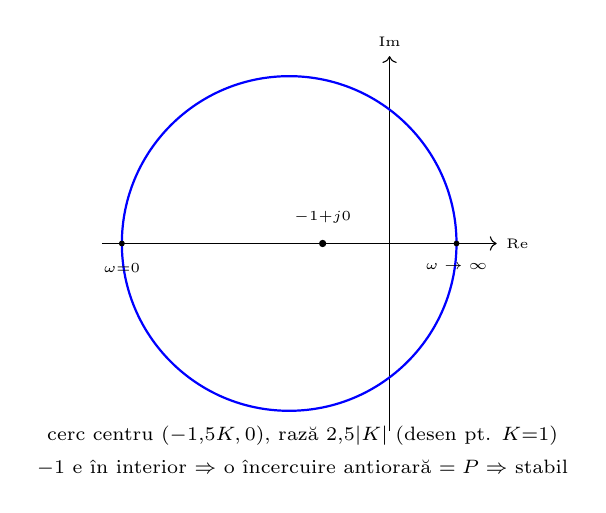
\begin{tikzpicture}[scale=0.85]
\draw[->] (-4.3,0) -- (1.6,0) node[right]{\tiny Re};
\draw[->] (0,-2.8) -- (0,2.8) node[above]{\tiny Im};
\draw[thick,blue] (-1.5,0) circle (2.5);
\filldraw (-1,0) circle (1.3pt); \node[above] at (-1,0.15){\tiny $-1{+}j0$};
\filldraw (-4,0) circle (1pt); \node[below] at (-4,-0.15){\tiny $\omega{=}0$};
\filldraw (1,0) circle (1pt); \node[below] at (1,-0.15){\tiny $\omega\to\infty$};
\node[align=center] at (-1.3,-3.1){\scriptsize cerc centru $(-1{,}5K,0)$, rază $2{,}5|K|$ (desen pt. $K{=}1$)\\\scriptsize $-1$ e în interior $\Rightarrow$ o încercuire antiorară $=P \Rightarrow$ stabil};
\end{tikzpicture}
\end{center}

\textbf{Subiect D — locul rădăcinilor, 4 poli reali, fără zerouri:} $G(s)H(s)=\dfrac{K}{(s+1)(s+2)(s+3)(s+4)}$ (reacție unitară).

\textit{Rezolvare (pașii \hyperref[sec:14]{secțiunii 14}):} (pasul 1) poli $-1,-2,-3,-4$, fără zerouri; (pasul 2) $n{=}4$ ramuri, $m{=}0$ (toate merg la $\infty$). Axa reală (pasul 3): segmentele $[-2,-1]$ și $[-4,-3]$. Asimptote (pasul 4, $\theta_k{=}\tfrac{180^\circ(2k+1)}{n-m}$, $\sigma_a{=}\tfrac{\sum p_i-\sum z_j}{n-m}$): $4$ asimptote, centrul $\sigma_a{=}\tfrac{-1-2-3-4}{4}{=}-2{,}5$, unghiuri $\pm45^\circ,\pm135^\circ$.

Puncte de ramificație (pasul 6, $dK/ds{=}0$ cu $K{=}{-}A(s)/B(s)$; $K{=}-(s{+}1)(s{+}2)(s{+}3)(s{+}4)$, notând $u{=}s^2{+}5s$: $K{=}-(u{+}4)(u{+}6)$, $dK/ds{=}0\Rightarrow u{+}5{=}0\Rightarrow s^2{+}5s{+}5{=}0$): $s_{1,2}{=}\tfrac{-5\pm\sqrt5}2\approx-1{,}38$ și $-3{,}62$ (ambele pe segmentele găsite, deci valide) — la ambele, prin simetrie față de $\sigma_a$, $K{=}1$.

Intersecția cu axa $j\omega$ (pasul 7, criteriul Routh): ecuația caracteristică $s^4{+}10s^3{+}35s^2{+}50s{+}(24{+}K){=}0$; tabloul Routh dă:
\begin{keyeq}\color{red!65!black}
$$K_l=126,\qquad s=\pm j\sqrt5\approx\pm j2{,}24$$
\end{keyeq}

\begin{center}
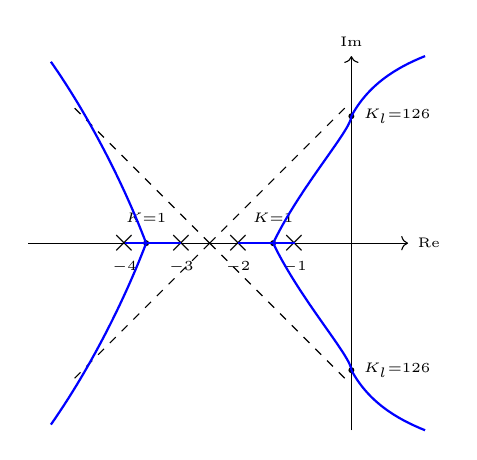
\begin{tikzpicture}[scale=0.72]
\draw[->] (-5.7,0) -- (1,0) node[right]{\tiny Re};
\draw[->] (0,-3.3) -- (0,3.3) node[above]{\tiny Im};
\node at (-1,0){\large$\times$}; \node[below] at (-1,-0.15){\tiny $-1$};
\node at (-2,0){\large$\times$}; \node[below] at (-2,-0.15){\tiny $-2$};
\node at (-3,0){\large$\times$}; \node[below] at (-3,-0.15){\tiny $-3$};
\node at (-4,0){\large$\times$}; \node[below] at (-4,-0.15){\tiny $-4$};
\filldraw (-1.38,0) circle (1.2pt); \node[above] at (-1.38,0.2){\tiny $K{=}1$};
\filldraw (-3.62,0) circle (1.2pt); \node[above] at (-3.62,0.2){\tiny $K{=}1$};
\filldraw (0,2.24) circle (1.2pt); \node[right] at (0.05,2.24){\tiny $K_l{=}126$};
\filldraw (0,-2.24) circle (1.2pt); \node[right] at (0.05,-2.24){\tiny $K_l{=}126$};
\draw[dashed] (-2.5,0)--(-0.1,2.4); \draw[dashed] (-2.5,0)--(-4.9,2.4);
\draw[dashed] (-2.5,0)--(-0.1,-2.4); \draw[dashed] (-2.5,0)--(-4.9,-2.4);
\draw[thick,blue] (-1,0) -- (-1.38,0); \draw[thick,blue] (-2,0) -- (-1.38,0);
\draw[thick,blue] (-1.38,0) .. controls (-0.9,1) and (0,2) .. (0,2.24);
\draw[thick,blue] (0,2.24) .. controls (0.3,2.8) and (0.8,3.1) .. (1.3,3.3);
\draw[thick,blue] (-1.38,0) .. controls (-0.9,-1) and (0,-2) .. (0,-2.24);
\draw[thick,blue] (0,-2.24) .. controls (0.3,-2.8) and (0.8,-3.1) .. (1.3,-3.3);
\draw[thick,blue] (-3,0) -- (-3.62,0); \draw[thick,blue] (-4,0) -- (-3.62,0);
\draw[thick,blue] (-3.62,0) .. controls (-4,1) and (-4.6,2.2) .. (-5.3,3.2);
\draw[thick,blue] (-3.62,0) .. controls (-4,-1) and (-4.6,-2.2) .. (-5.3,-3.2);
\end{tikzpicture}
\end{center}

\textbf{Subiect E — răspuns la intrare sinusoidală, exact la rezonanță:} $G_0(s)=\dfrac{25}{s^2+6s+25}$ (circuit închis), $u(t)=6\sin5t$.

Formula generală (\hyperref[sec:6]{secțiunea 6}): $y_{st}(t)=U|G_0(j\omega)|\sin(\omega t+\varphi)$. Pentru un sistem de ordin 2 standard $G_0(s)=\dfrac{\omega_n^2}{s^2+2\zeta\omega_ns+\omega_n^2}$, evaluat exact la $\omega{=}\omega_n$ (rezonanța ideală nedeplasată — \hyperref[sec:12]{secțiunea 12}), numitorul devine $-\omega_n^2+\omega_n^2+j2\zeta\omega_n^2=j2\zeta\omega_n^2$, deci $G_0(j\omega_n)={-}j/(2\zeta)$ — formulă generală, valabilă pentru orice $\zeta,\omega_n$.

\textit{Aplicare:} formă standard $\omega_n^2{=}25\Rightarrow\omega_n{=}5$, $2\zeta\omega_n{=}6\Rightarrow\zeta{=}0{,}6$; intrarea are $\omega{=}5{=}\omega_n$ (exact rezonanță). La $s{=}j5$: numitor $={-}25{+}25{+}30j{=}30j\Rightarrow G_0(j5){=}25/30j{=}{-}j\tfrac56$ (confirmă formula generală $G_0(j\omega_n){=}{-}j/(2\zeta){=}{-}j/1{,}2={-}j\tfrac56$), deci $|G_0(j5)|=\dfrac1{2\zeta}=\dfrac56\approx0{,}833$, $\varphi=-90^\circ$:
\begin{keyeq}\color{red!65!black}
$$y_{st}(t)=6\cdot\dfrac56\sin(5t-90^\circ)=5\sin(5t-90^\circ)=-5\cos(5t)$$
\end{keyeq}

\begin{center}
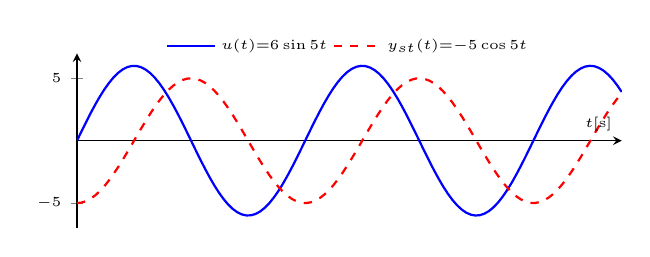
\begin{tikzpicture}
\begin{axis}[width=8.5cm,height=3.8cm,axis lines=middle,xlabel={\tiny $t$[s]},xtick=\empty,ytick={-5,5},yticklabels={\tiny$-5$,\tiny$5$},ymin=-7,ymax=7,xmin=0,xmax=3,
legend style={font=\tiny,at={(0.5,1.15)},anchor=north,legend columns=2,draw=none}]
\addplot[domain=0:3,samples=120,blue,thick] {6*sin(5*x*180/pi)};
\addplot[domain=0:3,samples=120,red,thick,dashed] {-5*cos(5*x*180/pi)};
\legend{$u(t){=}6\sin5t$,$y_{st}(t){=}{-}5\cos5t$}
\end{axis}
\end{tikzpicture}
\end{center}
\tip{\textit{Observație desen:} ieșirea (roșu) e defazată cu exact un sfert de perioadă ($-90^\circ$) în urma intrării (albastru) și are amplitudinea redusă de $2\zeta$ ori — comportament tipic \textbf{la rezonanță}.}

\begin{keyeq}\color{red!65!black}
\textbf{Teorie (bilet reluare toamnă 2025):}
\begin{enumerate}
\item unghiul de fază pentru factorul de amplificare $K$ (element pur proporțional): $\varphi{=}0^\circ$ dacă $K{>}0$; $\varphi{=}180^\circ$ dacă $K{<}0$ — constant, independent de $\omega$ (\hyperref[sec:7]{secțiunea 7}).
\item vârful de rezonanță pentru un sistem de \textbf{ordinul întâi}: \textbf{nu există} — $|G(j\omega)|{=}1/\sqrt{1{+}(\omega T)^2}$ e monoton descrescătoare de la $\omega{=}0$ $\Rightarrow M_r{=}1$ (rezonanța apare doar la ordinul 2, cu $\zeta\le0{,}707$ — \hyperref[sec:12]{secțiunea 12}).
\item sistem cu \textbf{dublu integrator} în bucla deschisă (tip $\nu{=}2$): eroare staționară \textbf{finită} doar la intrare \textbf{parabolă/accelerație} ($K_a$ finit); la treaptă și rampă $e_{ss}{=}0$ (\hyperref[sec:18]{secțiunea 18}).
\item schema bloc de reglare pentru sistem MIMO (2 intrări–2 ieșiri) — vezi desenul din \hyperref[sec:19]{secțiunea 19} (Teorie, pct. 4).
\end{enumerate}
\end{keyeq}

\section*{22. Bilet suplimentar — sesiunea 2024}\phantomsection\label{sec:22}
\textit{Al treilea bilet TS2 găsit (pe lângă cele din \hyperref[sec:21]{secțiunea 21} și \hyperref[sec:19]{secțiunea 19}) — structură diferită (3 subiecte + 10 întrebări de teorie), cu un subiect de ecuație diferențială și unul de reducere a schemelor bloc cu bucle multiple, ambele fără echivalent exact în restul documentului.}

\textbf{Subiect 1 — ecuație diferențială, condiții inițiale nule (1.5p):} $y^{(2)}(t)+4y^{(1)}(t)+5y(t)=2t$.

\textit{Rezolvare (Laplace + fracții simple, \hyperref[sec:3b]{secțiunea 3b}):} aplic transformata Laplace cu $y(0){=}y'(0){=}0$ și $\mathcal L\{t\}{=}1/s^2$:
$$s^2Y(s)+4sY(s)+5Y(s)=\dfrac2{s^2}\ \Rightarrow\ Y(s)=\dfrac2{s^2(s^2+4s+5)}$$
Numitorul are un pol dublu în $s{=}0$ și un factor pătratic ireductibil ($s^2{+}4s{+}5$, discriminant $16{-}20{<}0$, poli $-2{\pm}j$) — descompun (\hyperref[sec:3b]{secțiunea 3b}):
$$Y(s)=\dfrac As+\dfrac B{s^2}+\dfrac{Cs+D}{s^2+4s+5}$$
Identific coeficienții: din $s^0$: $B{=}2/5{=}0{,}4$; din $s^1$: $5A{+}4B{=}0\Rightarrow A{=}{-}0{,}32$; din $s^3$: $C{=}{-}A{=}0{,}32$; din $s^2$: $D{=}{-}4A{-}B{=}0{,}88$. Aduc ultimul termen la pătrat perfect, $s^2{+}4s{+}5{=}(s{+}2)^2{+}1$, și scriu numărătorul în funcție de $(s{+}2)$:
$$0{,}32s+0{,}88=0{,}32(s+2)+0{,}24$$
\begin{keyeq}\color{red!65!black}
$$y(t)=\underbrace{e^{-2t}(0{,}32\cos t+0{,}24\sin t)}_{\text{răspuns tranzitoriu}}+\underbrace{0{,}4t-0{,}32}_{\text{răspuns permanent}},\qquad t\ge0$$
\end{keyeq}
\tip{\textit{Observație:} spre deosebire de un răspuns la treaptă, aici răspunsul permanent NU e constant — intrarea e o rampă ($2t$) și sistemul n-are integrator, deci partea permanentă „urmărește" rampa, cu pantă $0{,}4$ și un decalaj $-0{,}32$; partea tranzitorie se stinge exponențial ($e^{-2t}$) și e oscilantă (poli complecși $-2{\pm}j$ ai sistemului omogen).}

\textbf{Subiect 2 — sistem de reglare cu buclă internă (2p total, pe sub-puncte):} partea fixă are o buclă internă (bloc direct $k_1/(s{+}3)$, reacție $k_2$ — vezi schema din enunț); peste ea se adaugă un regulator $G_R(s){=}1/s$, în buclă exterioară cu reacție negativă unitară.

\textit{a) Schema completă de reglare și funcția de transfer în circuit închis:} reduc întâi bucla internă (regulă generală buclă cu reacție, \hyperref[sec:2]{secțiunea 2}):
$$H_{fix}(s)=\dfrac{k_1/(s+3)}{1+k_1k_2/(s+3)}=\dfrac{k_1}{s+3+k_1k_2}$$

\begin{center}
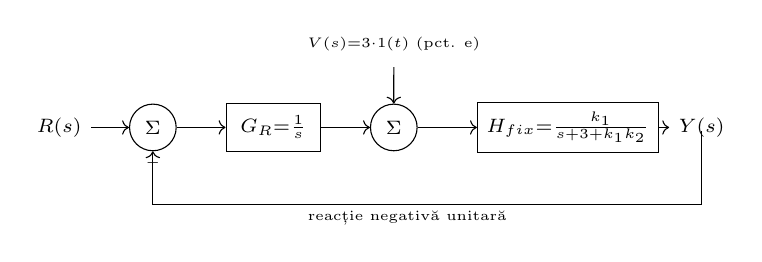
\begin{tikzpicture}[scale=0.85, every node/.style={font=\scriptsize}]
\node (r) at (0,0) {$R(s)$};
\node[draw,circle,minimum size=0.5cm] (s1) at (1.4,0) {$\Sigma$};
\draw[->] (r)--(s1);
\node[draw,minimum width=1.2cm,minimum height=0.6cm] (gr) at (3.2,0) {$G_R{=}\frac1s$};
\draw[->] (s1)--(gr);
\node[draw,circle,minimum size=0.5cm] (s2) at (5,0) {$\Sigma$};
\draw[->] (gr)--(s2);
\draw[->] (5,0.9)--(s2.north);
\node[above] at (5,1) {\tiny $V(s){=}3{\cdot}1(t)$ (pct. e)};
\node[draw,minimum width=2.1cm,minimum height=0.6cm] (hf) at (7.6,0) {$H_{fix}{=}\frac{k_1}{s+3+k_1k_2}$};
\draw[->] (s2)--(hf);
\node (y) at (9.6,0) {$Y(s)$};
\draw[->] (hf)--(y);
\draw[->] (9.6,-0.05) -- ++(0,-1.1) -| (s1.south);
\node[below] at (5.2,-1.1) {\tiny reacție negativă unitară};
\node[below] at (1.4,-0.3) {\tiny $-$};
\end{tikzpicture}
\end{center}
Funcția de transfer deschisă a buclei exterioare: $L(s){=}G_R(s)H_{fix}(s){=}\dfrac{k_1}{s(s+3+k_1k_2)}$, iar cea închisă:
\begin{keyeq}\color{red!65!black}
$$G_0(s)=\dfrac{L(s)}{1+L(s)}=\dfrac{k_1}{s^2+(3+k_1k_2)s+k_1}$$
\end{keyeq}

\textit{b) $k_1,k_2$ din $\zeta{=}0{,}7,\omega_n{=}3$:} identific cu forma standard $s^2{+}2\zeta\omega_ns{+}\omega_n^2$ (\hyperref[sec:12]{secțiunea 12}): $\omega_n^2{=}k_1\Rightarrow k_1{=}9$; $2\zeta\omega_n{=}3{+}k_1k_2\Rightarrow4{,}2{=}3{+}9k_2$:
\begin{keyeq}\color{red!65!black}
$$k_1=9,\qquad k_2=\dfrac{1{,}2}9\approx0{,}133$$
\end{keyeq}

\textit{c) Tip de intrare cu eroare staționară finită:} $L(s){=}\dfrac9{s(s+4{,}2)}$ are UN integrator (tip $1$) $\Rightarrow$ (\hyperref[sec:18]{secțiunea 18}) eroare finită doar la \textbf{intrare rampă}: $K_v{=}\lim_{s\to0}sL(s){=}9/4{,}2{\approx}2{,}14\Rightarrow e_{ss}(\text{rampă}){\approx}0{,}467$ (la treaptă $e_{ss}{=}0$).

\textit{d) Indicatorii de calitate în domeniul timpului} (formule generale, \hyperref[sec:12b]{secțiunea 12b}). \textit{Aplicare} ($\zeta{=}0{,}7,\omega_n{=}3\Rightarrow\omega_d{\approx}2{,}14$):
\begin{keyeq}\color{red!65!black}
$$\sigma\approx4{,}6\%,\qquad t_p\approx1{,}47\text{s},\qquad t_s\approx1{,}90\text{s (2\%)},\qquad t_r\approx0{,}6\text{s}$$
\end{keyeq}
\begin{center}
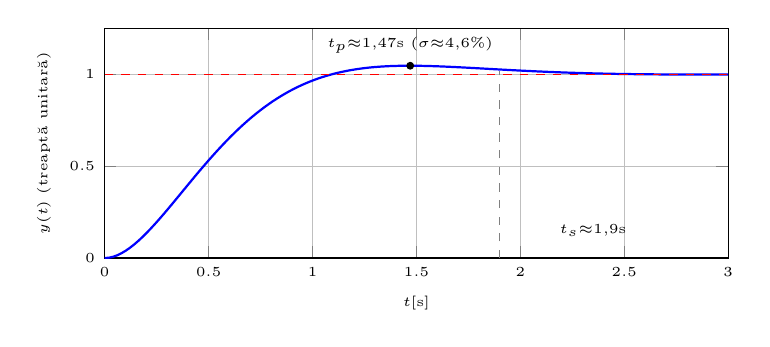
\begin{tikzpicture}
\begin{axis}[width=9.5cm,height=4.5cm,xlabel={\tiny $t$[s]},ylabel={\tiny $y(t)$ (treaptă unitară)},xmin=0,xmax=3,ymin=0,ymax=1.25,
grid=major,tick label style={font=\tiny}]
\addplot[domain=0:3,samples=150,blue,thick] {1-(1/0.7141)*exp(-2.1*x)*sin(2.1424*x*180/pi+45.57)};
\addplot[domain=0:3,samples=2,red,dashed] {1};
\addplot[only marks,mark=*,mark size=1.2pt,black] coordinates {(1.47,1.046)};
\node[font=\tiny] at (axis cs:1.47,1.16) {$t_p{\approx}1{,}47$s ($\sigma{\approx}4{,}6\%$)};
\draw[dashed,gray] (axis cs:1.9,0) -- (axis cs:1.9,1.02);
\node[font=\tiny] at (axis cs:2.35,0.15) {$t_s{\approx}1{,}9$s};
\end{axis}
\end{tikzpicture}
\end{center}

\textit{e) Perturbație treaptă $3{\cdot}1(t)$ la intrarea părții fixe} (adică imediat după $G_R$, marcată pe schema de mai sus): eroare la perturbație ($R{=}0$), $E(s){=}{-}H_{fix}(s)V(s)/[1{+}G_R(s)H_{fix}(s)]$ (din schemă, la fel ca deducerea din \hyperref[sec:18]{secțiunea 18} dar cu intrarea perturbației după regulator). \textit{Aplicare} ($V(s){=}3/s$, $H_{fix}(s){=}9/(s{+}4{,}2)$):
$$E(s)=\dfrac{-\frac9{s+4{,}2}\cdot\frac3s}{1+\frac9{s(s+4{,}2)}}=\dfrac{-27}{s^2+4{,}2s+9}$$
$E(s)$ nu mai are pol în $s{=}0$ (s-a simplificat) — deci, prin teorema valorii finale:
\begin{keyeq}\color{red!65!black}
$$e_{ss}(\text{perturbație})=\lim_{s\to0}sE(s)=0$$
\end{keyeq}
\textit{De ce:} integratorul din regulator ($G_R{=}1/s$) e plasat ÎNAINTE de punctul unde intră perturbația $\Rightarrow$ o respinge complet în regim staționar — regulă generală: orice perturbație treaptă care intră DUPĂ un integrator de pe calea directă e complet compensată static (eroarea ei tinde la $0$).

\textbf{Subiect 3 — funcție de transfer echivalentă, schemă cu 3 bucle (1.5p):} schema: $R(s)\to E$ se ramifică spre $G_1$ (către sumatorul $E_1$) și spre $G_3$ (cale feedforward, direct la sumatorul final, cu semn $-$); $E_1{=}G_1E-H_1Y_1$; $Y_1{=}G_2E_1$; $Y(s){=}Y_1-G_3E$; $H_2$ închide bucla exterioară de la $Y(s)$ înapoi la sumatorul lui $R$.

\textit{Rezolvare cu formula lui Mason (\hyperref[sec:4c]{secțiunea 4c}):} două căi directe: $P_1{=}G_1G_2$ (prin $G_1,G_2$) și $P_2{=}{-}G_3$ (feedforward). Trei bucle: $L_1{=}{-}G_2H_1$ (bucla $E_1{-}Y_1$, prin $H_1$), $L_2{=}{-}G_1G_2H_2$ (bucla exterioară completă), $L_3{=}G_3H_2$ (feedforward $+H_2$). $L_1$ (atinge doar $E_1,Y_1$) și $L_3$ (atinge doar $E,Y$) NU au niciun nod comun $\Rightarrow$ apar împreună (cu $+$) în $\Delta$:
$$\Delta=1-(L_1{+}L_2{+}L_3)+L_1L_3=1+G_2H_1+G_1G_2H_2-G_3H_2-G_2G_3H_1H_2$$
$\Delta_1{=}1$ (calea $P_1$ atinge toate cele trei bucle); $\Delta_2{=}1{-}L_1{=}1{+}G_2H_1$ (calea $P_2$ NU trece prin $E_1,Y_1$, deci nu atinge $L_1$):
\begin{keyeq}\color{red!65!black}
$$G_0(s)=\dfrac{Y(s)}{R(s)}=\dfrac{P_1\Delta_1+P_2\Delta_2}{\Delta}=\dfrac{G_1G_2-G_3-G_2G_3H_1}{1+G_2H_1+G_1G_2H_2-G_3H_2-G_2G_3H_1H_2}$$
\end{keyeq}
\textit{Verificare prin reducere algebrică directă} (aceeași schemă, fără Mason): din $Y_1{=}G_2E_1$ și $E_1{=}G_1E{-}H_1Y_1$ rezultă $Y_1{=}\dfrac{G_1G_2}{1+G_2H_1}E$; din $Y{=}Y_1{-}G_3E$, apoi $E{=}R{-}H_2Y$ înlocuit și izolat $Y/R$ — se obține EXACT aceeași fracție de mai sus. Cele două metode trebuie să dea mereu același rezultat; e o verificare bună de făcut pe hârtie dacă ai timp la examen.

\begin{keyeq}\color{red!65!black}
\textbf{Teorie (bilet 2024, 10 întrebări $\times$ pondere egală):}
\begin{enumerate}
\item pentru $G_0(s){=}2/(s{+}2)$ (ordinul unu, forma $a/(s{+}a)$): constanta de timp e $T{=}1/a{=}0{,}5$s (nu depinde de numărător, doar de polul $-a$).
\item la limita de stabilitate, polii sistemului închis sunt EXACT pe axa imaginară $j\omega$ (pereche $\pm j\omega_0$, sau un pol în origine) — niciun pol în semiplanul drept.
\item un sistem de ordinul întâi are răspuns MONOTON la treaptă (fără depășire) $\Rightarrow$ timpul de vârf $t_p$ \textbf{nu se definește} (conceptul e specific ordinului doi subamortizat, \hyperref[sec:12]{secțiunea 12}).
\item pentru $G_0(s){=}9/(s^2{+}3s{+}9)$: $\omega_n^2{=}9\Rightarrow\omega_n{=}3$; $2\zeta\omega_n{=}3\Rightarrow\zeta{=}0{,}5$.
\item schițarea răspunsului ordinul doi după $\zeta$: $\zeta{=}0$ — oscilație sinusoidală întreținută (neamortizată); $0{<}\zeta{<}1$ — oscilație amortizată exponențial, cu depășire (subamortizat); $\zeta{=}1$ — cea mai rapidă revenire FĂRĂ oscilație (critic amortizat); $\zeta{>}1$ — revenire lentă, monotonă (supraamortizat).
\item pentru ordinul 3, ecuație caracteristică $s^3{+}a_2s^2{+}a_1s{+}a_0{=}0$: limita de stabilitate (criteriul Routh, rândul $s^1$ nul) apare la $a_2a_1{=}a_0$.
\item impulsul Dirac e derivata treptei unitare, $\delta(t){=}\frac{d}{dt}1(t)$ (echivalent, treapta e integrala impulsului) — în Laplace: $\mathcal L\{\delta(t)\}{=}1$, $\mathcal L\{1(t)\}{=}1/s$.
\item regulatorul prelucrează eroarea (referință $-$ ieșire măsurată) și generează comanda aplicată procesului, ca să asigure performanțele impuse (stabilitate, eroare staționară mică/nulă, timp de răspuns, suprareglaj) — conține de regulă acțiune integratoare pentru eliminarea erorii staționare (exact rolul lui $G_R{=}1/s$ de la Subiectul 2).
\item $\mathcal L\{e^{-2t}\}=\dfrac1{s+2}$ (formulă directă, \hyperref[sec:3b]{secțiunea 3b}).
\item semnalul treaptă unitară întârziată $1(t-\tau)$: $0$ pentru $t{<}\tau$, salt vertical la $\tau$, apoi constant $1$ pentru $t{\ge}\tau$ (aceeași treaptă, doar deplasată la dreapta cu $\tau$).
\end{enumerate}
\end{keyeq}

\end{document}
